\documentclass[12pt, bibliography=totoc]{scrartcl}
\title{Predicting Blood Pressure from Photoplethysmogram Waveform Data: A Signal Processing and
Machine Learning Approach}
\author{Hugas Jasinskas}
\usepackage[utf8]{inputenc}
\usepackage{graphicx}
\usepackage{wrapfig}
\usepackage{url}
\usepackage{setspace}
\usepackage{tabto}
\usepackage[export]{adjustbox}
\usepackage{float}
\usepackage{csquotes}
\usepackage{amsmath}
\usepackage{multicol}
\usepackage{listings}
\usepackage{lstmisc}
\usepackage{array}
\usepackage{caption}
\usepackage{subcaption}
\usepackage{rotating}
\usepackage{hyperref}
\usepackage[table]{xcolor}
\usepackage{pgfplots}

\begin{document}

    \begin{titlepage}
        \begin{center}
            \vspace*{1cm}
            \begin{figure}[h]
                \centering
                
\includegraphics[scale=0.6]{images/hs/hd}
                
\includegraphics[scale=1]{images/hs/hhn}
                
\includegraphics[scale=0.06]{images/hs/tmu}
                \label{fig:unis}
            \end{figure}

            \vspace*{1cm}

            \Huge
            \textbf{Master's Thesis}

            \vspace{0.5cm}
            \Large
            Medical Informatics Master

            \vspace{0.5cm}
            \Large
            Universität Heidelberg / Hochschule Heilbronn

            \vspace{0.5cm}
            \Large
            in Cooperation with Taipei Medical University

            \hrulefill

            \vspace{1cm}

            \Huge
            \textbf{Predicting Blood Pressure from Photoplethysmogram Waveform Data: A Signal Processing and
            Machine Learning Approach}

        \end{center}

        \vfill
        \Large
        \noindent
        Supervisor: \tab\hspace{-2cm} Prof.\ Dr. Rolf Bendl\\
        Co-Supervisor: \tab\hspace{-2cm} Prof.\ Dr. Syed Abdul Shabbir\\
        Submitted by: \tab\hspace{-2cm} Hugas Jasinskas\\
        Matriculation number: \tab\hspace{-2cm} 202509\\
        Submitted on: \tab\hspace{-2cm} March 1st, 2024\\

    \end{titlepage}

    \newpage

    \begin{Huge}
        \centerline{Affidavit}
    \end{Huge}

    \vspace{2cm}

    \begin{Large}

        I hereby declare under oath that I have independently prepared the present work without using sources other than those indicated; any thoughts taken directly or indirectly from external sources (including electronic sources) are identified as such.

        The work has not been submitted to any examination authority, either domestic or foreign, in the same or similar form, and has not been published.

    \end{Large}

    \vfill

    \rule{4cm}{0.5mm} \tab \qquad \qquad \rule{4cm}{0.5mm}

    Date \tab \qquad \qquad Signature

    \newpage
    \doublespacing
    \tableofcontents

    \newpage
    \onehalfspacing


    \section{Abstract}\label{sec:abstract}


    \section{Introduction}
    \label{sec:introduction}
    \subsection{Subject and Motivation}
\label{subsec:subject_motivation}

Cardiovascular diseases (CVDs) are the leading cause of death worldwide, according to WHO publishing statistics~\cite{organizationWorldHealthStatistics2023}.
One of the main factors contributing to CVDs is Hypertension.
It is the leading risk factor for mortality, and is ranked third as a cause of disability-adjusted life-years~\cite{ezzatiSelectedMajorRisk2002}.
Currently, there is a significant need for continuous blood pressure (BP) monitoring due to various factors.
Primarily, while hypertension is a manageable condition, the availability of accurate high BP detection remains scarce, especially in low-resource environments~\cite{burtPrevalenceHypertensionUS1995}.
Additionally, blood pressure (BP) is subject to rapid fluctuations influenced by various factors, including stress, emotions, dietary intake, physical activity, and medication usage~\cite{poonCufflessNoninvasiveMeasurements2005}.
Continuous monitoring of blood pressure, rather than relying on isolated measurements, plays a vital role in the early detection and treatment of hypertension~\cite{el-hajjDeepLearningModels2021}.

The current accurate methods for measuring BP continuously are either invasive or involving a cuff-mechanism.
Catheterization is internationally recognized as the \enquote{gold standard} for obtaining the most accurate measurement of continuous blood pressure~\cite{sharmaCuffLessContinuousBlood2017}.
However, due to its invasive nature and limited applicability to hospital settings, this method requires medical intervention, which renders it inconvenient for everyday use.

While cuff-based devices are commonly utilized for this objective, it is worth noting that around 30\% of home blood pressure monitors are found to be inaccurate, rendering continuous measurement unfeasible~\cite{leungHypertensionCanada20162016, seboBloodPressureMeasurements2014}.
Moreover, this approach relies on the individual consciously and intentionally engaging in manual blood pressure monitoring, which poses limitations and might be often overlooked.

An ideal technology for measuring blood pressure should have the following attributes: non-invasiveness, cuffless operation, optical functionality, wearable design, and cost-effectiveness~\cite{el-hajjDeepLearningModels2021}.
One approach satisfying these requirements is the estimation of BP from a single measurement PPG sensor.
This approach, using two modes, reflectance and transmission, has gained an increasing amount of attention in the literature due its simplicity, and ability to provide continuous and cuffless measurement~\cite{el-hajjDeepLearningModels2021}.
Typically, the photoplethysmography (PPG) technique has been traditionally employed in healthcare settings to measure heart rate~\cite{reyesWirelessPhotoplethysmographicDevice2012} and blood oxygen saturation using a pulse oximeter~\cite{yoonMultipleDiagnosisBased2002}.

Nevertheless, establishing a straightforward, distinct, and continuous relationship between these characteristics and blood pressure (BP) has proven to be challenging.
To address this, the approach heavily depends on signal pre-processing techniques, extracting PPG features, and utilizing machine learning (ML) algorithms to estimate BP based on these features~\cite{el-hajjDeepLearningModels2021}.
A recent scoping review by Knight et al.\ concluded that PPG can be successfully used to continuously measure BP, by evaluating latest publications and finding over 80\% accuracy in detecting hypertension~\cite{knightAccuracyWearablePhotoplethysmography2022}.

This study examines the current methods and aims to develop efficient approaches for the continuous and accurate measurement of blood pressure using PPG and addresses the following research questions:

\begin{enumerate}
    \item \textbf{What is the relationship between PPG data and blood pressure among Intensive Care Unit (ICU) patients?}

    \item \textbf{Can PPG-based data be used to estimate blood pressure accurately?}

\end{enumerate}

\subsection{Tasks and Objectives}
\label{subsec:tasks_objectives}

The tasks of the thesis are as follows:

\begin{enumerate}
    \item Signal Processing: to find an optimal data fetching and filtering approach from available MIMIC Databases.
    \item Likewise, to create a consistent algorithm for key feature extraction.
    \item Machine Learning: to develop a model based on the resulting features from Signal Processing, to reliably predict BP from PPG\@.
\end{enumerate}

\subsection{Structure of the Thesis}
\label{subsec:structure}

This thesis is organized as follows:

In Chapter~\ref{sec:background}, the foundations of the used terms and prerequisites for the methods are explained.
For example, in~\ref{subsec:med_background}, the terms \enquote{Blood Pressure} (\ref{subsubsec:bp}) and \enquote{Photoplethysmography} (\ref{subsubsec:ppg}) are discussed.
Furthermore, the general structure of MIMIC databases is explained (\ref{subsubsec:mimic}).
In addition, the essential information about the Computing part of this research is provided (\ref{subsec:computing_background}).

In Chapter~\ref{sec:methods}, the methodology is explained.

Chapter~\ref{sec:results} presents the results.

The focus of Chapters~\ref{sec:discussion} and~\ref{sec:conclusion} is on summarizing the work.
Here, both the future prospects for this research field and the next steps in relation to broader scope projects are presented.


    \section{Theoretical Background}
    \label{sec:background}
    \subsection{Medical Background}
\label{subsec:med_background}

\subsubsection{Blood Pressure}
\label{subsubsec:bp}

% general BP
Blood pressure (BP) is a physiological measure of the force exerted by circulating blood against the walls of the arteries~\cite{WhatBloodPressure2019}.
It is highly dependent on blood flow, which refers to the movement of blood through a vessel, tissue, or organ.
Blood circulation begins with the contraction of the heart's ventricles.
This action generates a type of hydrostatic pressure, which is the force exerted by a fluid due to gravitational pull, typically against the walls of the container that confines it.

BP is a type of hydrostatic pressure, representing the force exerted by blood on the walls of blood vessels or the heart's chambers.
While it can be assessed in various body regions, the term \enquote{blood pressure} without specific qualifiers commonly refers to systemic arterial BP\@.
This denotes the pressure of blood within the arteries of the systemic circulation.
In clinical settings, this pressure is measured in millimeters of mercury (mmHg) and is typically acquired using the brachial artery in the arm~\cite{betts20BloodFlow2022}.

% measuring significance
Measuring BP is crucial for assessing cardiovascular health and identifying potential risks.
It allows for the early detection of conditions like hypertension and hypotension, enabling timely interventions to prevent serious cardiovascular events~\cite{naylorArterialCathetersEarly2020}.
BP serves as a key indicator of the risk for heart attacks, strokes, and heart failure, guiding preventive measures and treatment strategies~\cite{ettehadBloodPressureLowering2016}.

\vspace{0.2cm}
\textit{Various Types of Measurement}
\vspace{0.2cm}

% cuff BP measuring
One of the most common BP measurement methods is one using a sphygmomanometer (see manual~\ref{fig:sphyg} and automatic~\ref{fig:auto_sphyg} devices), also known as non-invasive blood pressure (NIBP), is typically recorded as numeric values at specific time intervals.
The process involves inflating the cuff to temporarily stop blood flow and then gradually releasing the pressure to detect the sounds associated with the flow of blood through the brachial artery.
Manually, the measurement entails one individual conducting the procedure on another, typically involving a healthcare professional administering the assessment to a patient.
Conversely, automatic measurement allows the patient to independently measure their blood pressure without external assistance.
Both approaches yield comparable measurements of the same nature.
The two primary values obtained are systolic pressure (maximum pressure during heartbeats) and diastolic pressure (minimum pressure between heartbeats).
During the process of cuff inflation and deflation, each heartbeat generates characteristic sounds (Korotkoff sounds) that are detected by a stethoscope placed over the brachial artery.
Systolic pressure is recorded when the first tapping sounds are heard, and diastolic pressure is recorded when the sounds disappear or change character.
This beat-to-beat approach provides information about individual fluctuations in blood pressure~\cite{betts20BloodFlow2022}.

\begin{figure}[h]
    \centering
    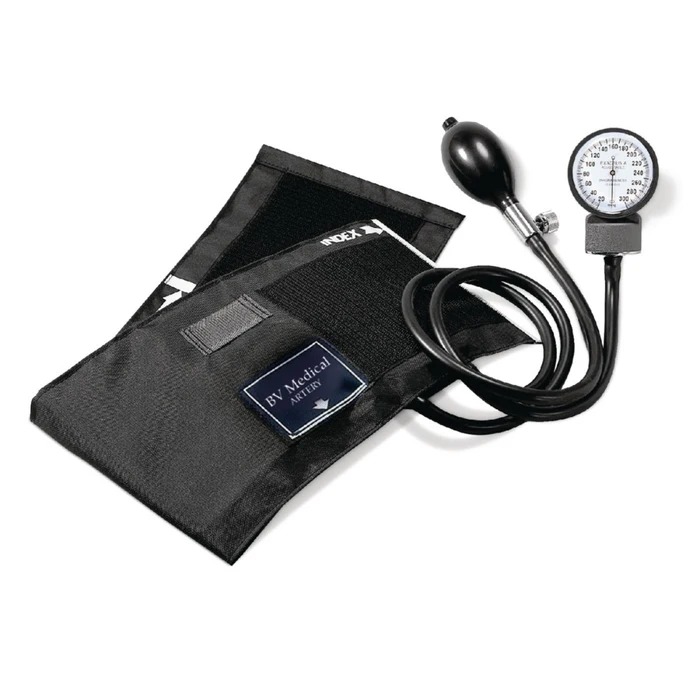
\includegraphics[scale=0.2]{images/abp/sphyg}
    \caption{Standard Sphygmanometer \cite{StandardSphygmomanometer}}
    \label{fig:sphyg}
    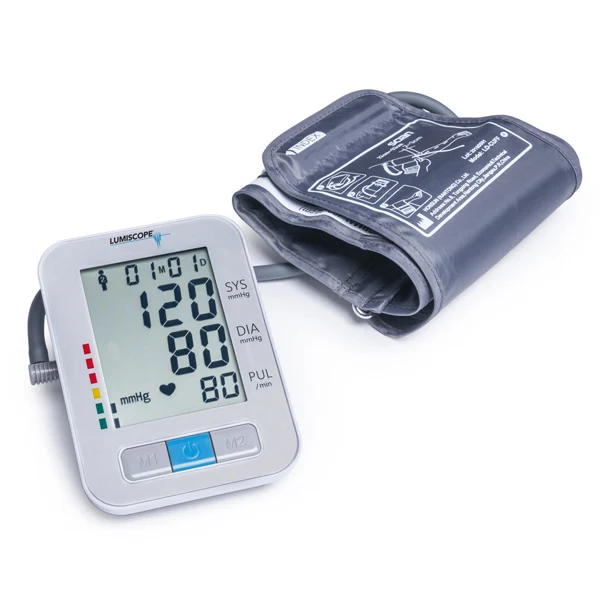
\includegraphics[scale=0.2]{images/abp/auto_sphyg}
    \caption{Automatic Digital Sphygmanometer \cite{AutomaticDigitalBlood}}
    \label{fig:auto_sphyg}
\end{figure}

Although measuring blood pressure with a cuff using a sphygmomanometer is widely adopted as a common and convenient method, it is not without its constraints.
Studies, such as those by Leung et al.\ and Sebo et al.\ , have highlighted the inability of home blood pressure monitoring devices to consistently and accurately detect hypertension~\cite{leungHypertensionCanada20162016, seboBloodPressureMeasurements2014}.
Furthermore, a significant limitation lies in its inability to provide continuous and consistent monitoring, necessitating patients to actively remember and engage in the effort to measure their blood pressure.
This intermittent approach using a cuff provides valuable insights into systolic and diastolic pressures at specific time intervals, but it may not capture the nuanced changes that occur between measurements.
To address the need for continuous monitoring, other methods, such as arterial catheterization, are employed.

% arterial BP
Arterial catheterization (illustrated in Figure~\ref{fig:catheter}) is commonly employed in critical patient care, serving dual purposes: continuous blood pressure monitoring and obtaining frequent blood gas measurements.
Typically conducted at bedside, the procedure utilizes percutaneous methods like the Seldinger technique to cannulate arteries~\cite{clarkArterialCatheterization1992}.
The resulting arterial blood pressure (ABP) is a dynamic parameter that can change with each heartbeat, and it is typically represented as a waveform rather than a single numeric value.
The ABP waveform consists of two main components: systolic pressure and diastolic pressure.
Such continuous monitoring of ABP is usually done in clinical settings, using an arterial line connected to a pressure transducer.
The resulting waveform is displayed on a monitor in real-time.
However, for ease of interpretation and documentation, numeric values are commonly extracted from the waveform at specific time intervals~\cite{hillImputationContinuousArterial2021}.

\begin{figure}[h]
    \centering
    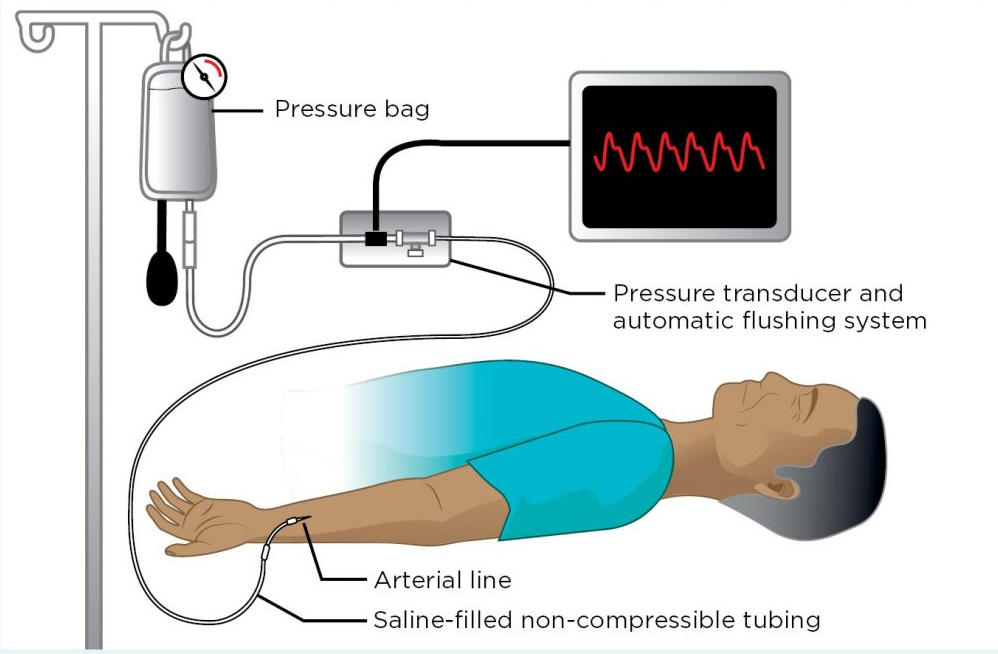
\includegraphics[scale=0.4]{images/abp/catheter}
    \caption{Arterial Catheterization and Stationary BP Monitoring~\cite{contributorEssentialCriticalCare2021}}
    \label{fig:catheter}
\end{figure}

In situations where high temporal resolution is crucial, ABP can be recorded beat-to-beat, providing a value for each heartbeat.
This is particularly important in situations where rapid changes in blood pressure need to be closely monitored, such as during certain medical procedures or in critically ill patients~\cite{lehmanMethodsBloodPressure2013}.

For routine monitoring and documentation, numeric values are often averaged over a specific time interval, such as every 1, 5, or 15 minutes.
This averaged value may be reported as the mean arterial pressure (MAP), which is a weighted average of the systolic and diastolic pressures over a cardiac cycle~\cite{demersPhysiologyMeanArterial2024}
Some monitoring systems may also provide systolic and diastolic blood pressure readings at regular intervals.

Alternative approaches for measuring BP have emerged over the past years.
Volume clamping~\cite{kimBallistocardiogramBasedApproachCuffless2018} and tonometry~\cite{imholzFifteenYearsExperience1998} are some of the other methods.
These non-invasive techniques offer continuous monitoring of blood pressure values.
Volume clamping, which involves the use of a small finger cuff and a PPG sensor, is one method for continuous blood pressure measurement.
Tonometry, on the other hand, is a cuffless approach that utilizes a manometer-tipped probe pressed directly on an artery.
The volume clamping approach allows for instantaneous and prolonged blood pressure measurement.
However, it is associated with high costs and still necessitates the use of a cuff, which can be inconvenient and uncomfortable.
Conversely, the tonometry method is sensitive to movement of the arm and probe, making it challenging to maintain accuracy in practical applications.
Additionally, constant calibration with a cuff blood pressure device is required~\cite{peterReviewMethodsNoninvasive2014}.

\vspace{0.2cm}

In conclusion, blood pressure serves as a critical physiological measure, representing the force exerted by blood on the walls of blood vessels.
The conventional method of measuring blood pressure with a cuff and sphygmomanometer provides valuable insights into systolic and diastolic pressures but is limited by its intermittent nature.
To address the need for continuous monitoring, arterial catheterization is commonly employed in critical care, offering real-time data through a dynamic waveform.
Alternative non-invasive approaches like volume clamping and tonometry aim to provide continuous blood pressure monitoring, but they come with their own challenges and considerations.
As technology advances, these methods contribute to a comprehensive understanding of blood pressure dynamics, facilitating improved patient care and risk assessment.

\subsubsection{Photoplethysmography}
\label{subsubsec:ppg}

% meaning and basic information
Photoplethysmography (PPG) is an optical measurement technique designed to identify changes in blood volume within the microvascular bed of tissue~\cite{challonerPhotoelectricPlethysmographMeasurement1974}.
Its clinical application is extensive, as the technology is integrated into commercially available medical devices, including pulse oximeters, vascular diagnostics, and digital beat-to-beat blood pressure measurement systems.
The fundamental structure of PPG technology is straightforward, requiring only a few opto-electronic components: a light source for tissue illumination, usually a light-emitting diode (LED) and a photodiode (PD) to gauge slight variations in light intensity correlated with changes in perfusion in the catchment volume.

% history and origins
\vspace{0.2cm}
\textit{History}
\vspace{0.2cm}

One of the first mentioned instances on the use of PPG were recorded in 1936 by Molitor and Kniazuk~\cite{molitorNewBloodlessMethod1936}.
They outlined comparable devices employed for tracking alterations in blood volume in the rabbit ear under conditions of venous occlusion and the administration of vasoactive drugs.
A pioneer who helped establish the PPG technique was Alrick Hertzman~\cite{hertzmanPhotoelectricPlethysmographyFingers1937}.
In his 1937 paper, Hertzman coined the term \enquote{Photoelectric Plethysmograph} etymologically meaning:
photo - \enquote{light}, plethora - \enquote{exess of body fluid, blood}, graph - \enquote{something written}.
He detailed the application of a reflection mode system to assess alterations in blood volume within the fingers, particularly during the Valsalva maneuver~\cite{srivastavValsalvaManeuver2024}, exercise, and exposure to cold.
This contribution not only demonstrated the versatility of the technique but also underscored its potential clinical relevance.

Hertzman and Spealman~\cite{hertzmanPhotoelectricPlethysmographyFingers1937} outlined two crucial features of the PPG pulse waveform.
They categorized the pulse appearance into two phases: the anacrotic phase representing the ascending edge of the pulse, and the catacrotic phase representing the descending edge of the pulse.
The initial phase primarily corresponds to systole, while the subsequent phase relates to diastole and wave reflections from the periphery.
In individuals with healthy compliant arteries, a dicrotic notch is commonly observed during the catacrotic phase.

In the late 1970s, there arose a renewed interest in the PPG technology, driven by the demand for compact, dependable, cost-effective, and user-friendly noninvasive cardiovascular assessment techniques~\cite{yoshiyaSpectrophotometricMonitoringArterial1980}.
The progress in opto-electronics and clinical instrumentation has played a significant role in advancing PPG technology.
Semiconductor advancements, particularly in LEDs, photodiodes, and phototransistors, have brought about substantial improvements in the size, sensitivity, reliability, and reproducibility of PPG probe design.
A significant leap in the clinical application of PPG-based technology occurred with the introduction of the pulse oximeter~\cite{aoyagiPulseOximetryIts2002}.
This device revolutionized non-invasive monitoring of patients' arterial oxygen saturation, marking a major advancement in the field.

Other emerging technologies encompass PPG imaging technology, telemedicine, and remote monitoring.
In 2005, Wieringa et al.\ detailed a contactless multiple-wavelength PPG imaging system designed primarily for remotely imaging the distribution of arterial oxygen saturation (SpO2) within tissue~\cite{wieringaContactlessMultipleWavelength2005}.
The system captures movies of two-dimensional matrix spatially resolved PPG signals at different wavelengths during respiratory changes.
PPG was found to have substantial potential in telemedicine, particularly for remote/home health monitoring of patients.
Miniaturization, user-friendliness, and robustness stand as pivotal design criteria for such systems.
This is exemplified by finger ring-based PPG sensors for monitoring beat-to-beat pulsations (\cite{rheeArtifactresistantPowerefficientDesign2001}, ~\cite{zhengRingtypeDeviceNoninvasive2003}).

Most PPG devices these days either use the transmissive or reflective operating modes (illustrated in Figure~\ref{fig:reflection}).
Currently, the prevalent method is the transmissive mode, chosen for its notable accuracy and stability~\cite{leeReflectancePulseOximetry2016}.
However, there is a growing interest in reflective-mode PPG due to its elimination of the need for a thin measurement site.
This method proves versatile, applicable to various sites such as the feet, forehead, chest, and wrists.
Especially when the wrist serves as the designated measurement site, PPG sensors can be conveniently employed in the form of a band or watch.

\begin{figure}[h]
    \centering
    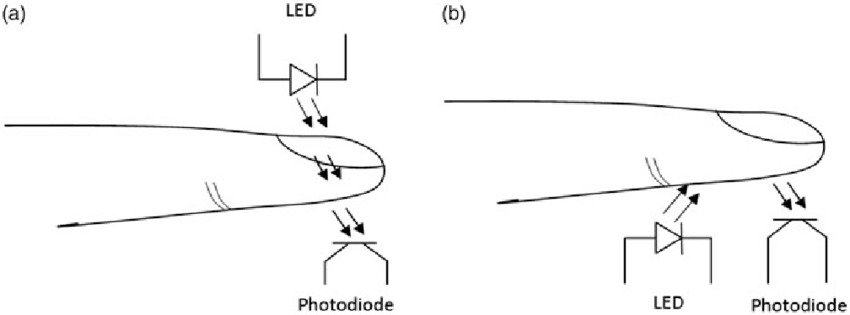
\includegraphics[scale=0.4]{images/ppg/reflection}
    \caption{PPG Transmission (a) and Reflection (b) operating modes \cite{mohanSpotMeasurementHeart2016}}
    \label{fig:reflection}
\end{figure}

% how does it work
\vspace{0.2cm}
\textit{Working Principle}
\vspace{0.2cm}

The PPG signal consists of pulsate (AC) and superimposed (DC) components (see Figure~\ref{fig:acdc}).
The AC component originates from variations in blood volume associated with heartbeats,
while the DC component is influenced by factors such as respiration, sympathetic nervous system activity, and temperature regulation~\cite{allenPhotoplethysmographyItsApplication2007a}.
The AC component specifically illustrates changes in blood volume during phasic cardiac activity, representing both the systolic and diastolic phases.
The systolic phase, also known as the \enquote{rise time} initiates with a valley and concludes at the pulse wave systolic peak.
The pulse wave concludes with another valley at the end of the diastolic phase~\cite{weisslerSystolicTimeIntervals1968}.
In most PPG waveform analyses including this one, the AC component in the form of a waveform signal is used.

\begin{figure}[h]
    \centering
    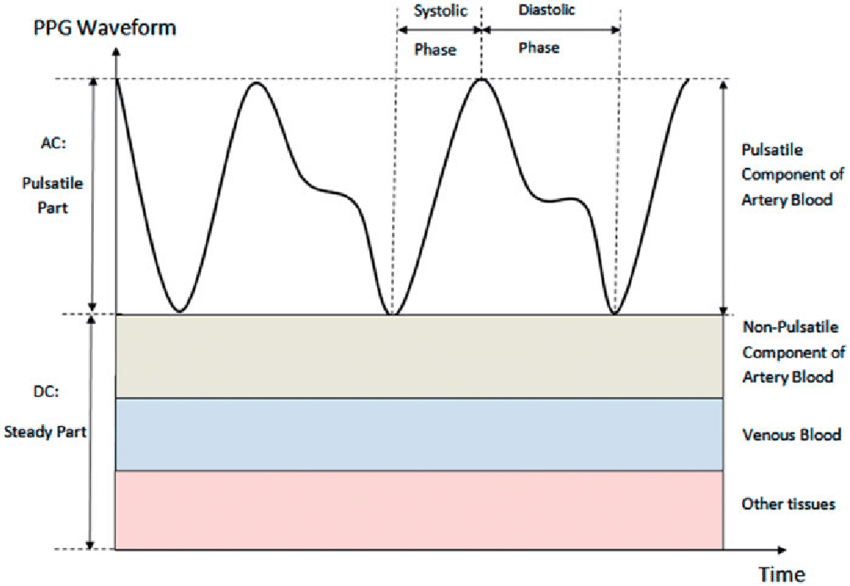
\includegraphics[scale=0.5]{images/ppg/ac+dc}
    \caption{AC and DC components of the PPG signal \cite{mohanSpotMeasurementHeart2016}}
    \label{fig:acdc}
\end{figure}

% main and potential use cases
\vspace{0.2cm}
\textit{Use Cases}
\vspace{0.2cm}

PPG finds diverse applications in clinical settings, covering physiological monitoring (such as blood oxygen saturation and heart rate), vascular assessment (including arterial disease, aging and tissue viability), and autonomic function evaluations (such as thermoregulation, heart rate and other assessments of cardiovascular variability)~\cite{allenPhotoplethysmographyItsApplication2007a}.
Furthermore, the popularity of PPG technology as an alternative for monitoring heart rate has risen recently, primarily attributed to its ease of use, user-friendly wearing comfort, and cost-effectiveness~\cite{sviridovaHumanPhotoplethysmogramNew2015}.
Nowadays, almost every wearable devices uses the PPG technology to track the user's heart rate and other extractable vital parameters~\cite{castanedaReviewWearablePhotoplethysmography2018}.
PPG sensors in mobile and wearable devices typically feature red, green, or both light-emitting diodes.
Most devices incorporate a green-light PPG sensor for continuous heart rate monitoring during daily activities.
Some devices also include red-light PPG sensors, which are effective for measuring heart rate when a person is stationary, providing insights into hydration, muscle saturation, and total hemoglobin.
While red-light PPG can penetrate tissue layers more deeply using near-infrared spectroscopy, it is susceptible to disturbance from ambient light.
In contrast, green light, being less absorbed by the skin, minimizes the impact of ambient light noise on the heart rate signal.
As a result, wearable devices commonly utilize green light rather than red-light PPG~\cite{ponnadaTechnologicalConsiderationsSensorassisted2019}.
Different types of devices implement the PPG technology.
It can be found in pulse oximeters, smartphones, smartwatches and other wearable devices (examples in Figure~\ref{fig:ppg-devices}).

\begin{figure}[h]
    \centering
    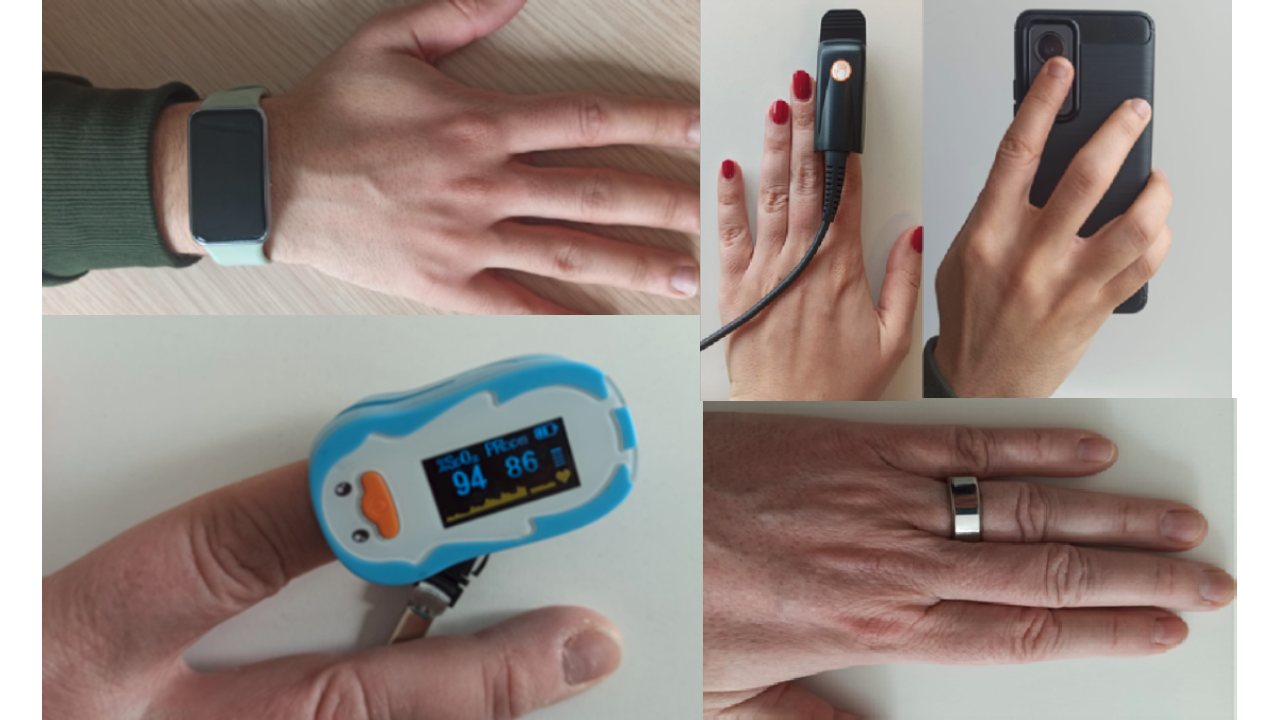
\includegraphics[scale=0.35]{images/ppg/ppg-devices}
    \caption{AC and DC components of the PPG signal \cite{zanelliPotentialAIBased2023}}
    \label{fig:ppg-devices}
\end{figure}

% Conclusion parahraph
\vspace{0.2cm}

In conclusion, the PPG is an optical sensor, consisting of an LED paired with a PD, hence it is simple, inexpensive and can be easily build into a wearable device.
The PPG waveform can be obtained using two modes, reflectance and transmission.
This waveform corresponds to the blood volume in blood vessels.
Traditionally employed in healthcare for heart rate and blood oxygen saturation measurements, particularly with pulse oximeters, the PPG plays a pivotal role~\cite{allenPhotoplethysmographyItsApplication2007a}.

% outlook to SP and ML
Additionally, peripheral volumetric changes exhibit correlation with BP~\cite{langewoutersPressurediameterRelationshipsSegments1986}.
Utilizing characteristic PPG features, ML functions can estimate Systolic BP (SBP) and Diastolic BP (DBP).
However, establishing a simple, clear, and continuous relationship between these features and BP remains elusive.
This method heavily relies on signal pre-processing, feature extraction, and the application of ML algorithms for BP estimation based on these features.

\subsubsection{MIMIC Databases}
\label{subsubsec:mimic}

Patient records and documentation are crucial for maintaining a comprehensive overview of medical history, aiding in accurate diagnosis, treatment planning, and ensuring continuity of care.
They also serve as legal documents, providing evidence of the care provided and facilitating communication among healthcare professionals.
Collecting digital data during routine clinical practice has become widespread across hospitals.
Over time, a pattern has emerged in the collection and storage of patient data for subsequent utilization in future research endeavors.

% History and Origin
\vspace{0.2cm}
\textit{Origin}
\vspace{0.2cm}

In 1996, two researchers at the Massachusetts Institute of Technology, George B. Moody and Roger G. Mark, introduced the Multiparameter Intelligent Monitoring in Intensive Care (MIMIC) Database (DB).
The DB was derived from patient monitors in the medical, surgical, and cardiac ICUs of Boston’s Beth Israel Hospital~\cite{moodyDatabaseSupportDevelopment1996}.
The first instance of the DB included 100 patient records, each typically containing between 24 and 48 hours of continuous recorded data.
The second version of the DB (MIMIC-II) was introduced in 2011 boasting a notably larger sample size and a wider scope of information sourced entirely from diverse digital information systems~\cite{saeedMultiparameterIntelligentMonitoring2011}.
MIMIC-III~\cite{johnsonMIMICIIIFreelyAccessible2016} was finalized in 2016, marking a significant expansion from MIMIC-II, with data available from over 40,000 patients.
The fourth and latest MIMIC DB was publicly released in 2023 spanning a decade of admissions from 2008 to 2019.
MIMIC-IV was announced to enhance the realm of publicly accessible critical care datasets, by integrating precise digital sources like the electronic medicine administration record and featuring a modular structure enabling seamless integration with external departments and diverse data modalities~\cite{johnsonMIMICIVFreelyAccessible2023}.
The diagram in Figure~\ref{fig:mimic_workflow} depicts the component interaction for data and information delivery to the publicly available DB\@.

\begin{figure}[h]
    \centering
    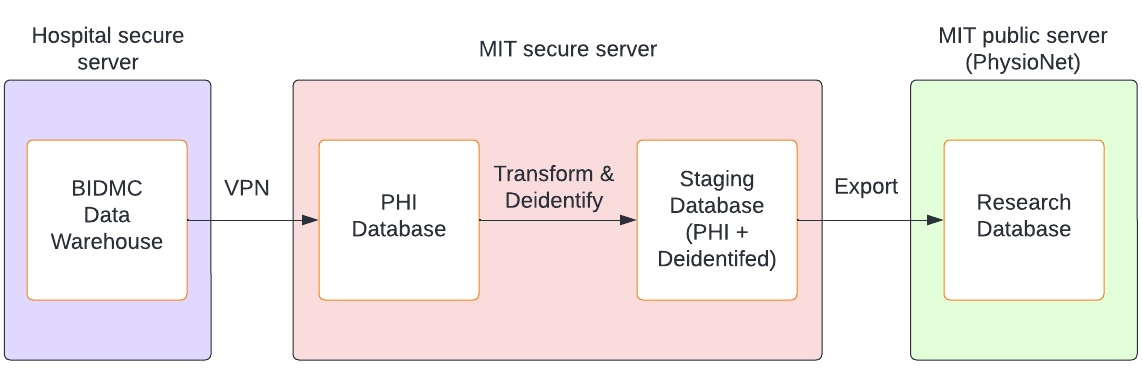
\includegraphics[scale=0.6]{images/mimic/mimic_workflow}
    \caption{Workflow between Beth Israel Deaconess Medical Center (BIDMC), Protected Health Information (PHI) DB ~\cite{charltonMIMICWFDBTutorials2022}}
    \label{fig:mimic_workflow}
\end{figure}

% Structure of MIMIC DB
\vspace{0.2cm}
\textit{Structure}
\vspace{0.2cm}

Both the MIMIC-III and MIMIC-IV DBs are cited and employed in this investigation, exhibiting comparable structures (depicted in Figure~\ref{fig:mimic_structure}), encompassing diverse data categories.
However, the primary emphasis of this inquiry lies in the Waveform Section of the DB (highlighted by a red rectangle in Figure~\ref{fig:mimic_structure}).
The waveform DB comprises individual records, each representing a patient's ICU stay and stored in a distinct subdirectory.
These records lack specific date or time data to ensure patient anonymity, relying instead on elapsed time from the record's start.
Supplemented by surrogate date and time information for cross-referencing with other DB modules.
Waveforms denote regularly sampled, high-resolution measurements stored in a signal specific numerical format.
To optimize storage and processing, these waveforms are segmented into intervals, maintaining continuous sampling within each segment despite potential signal unavailability throughout a patient's ICU stay.

\begin{figure}[h]
    \centering
    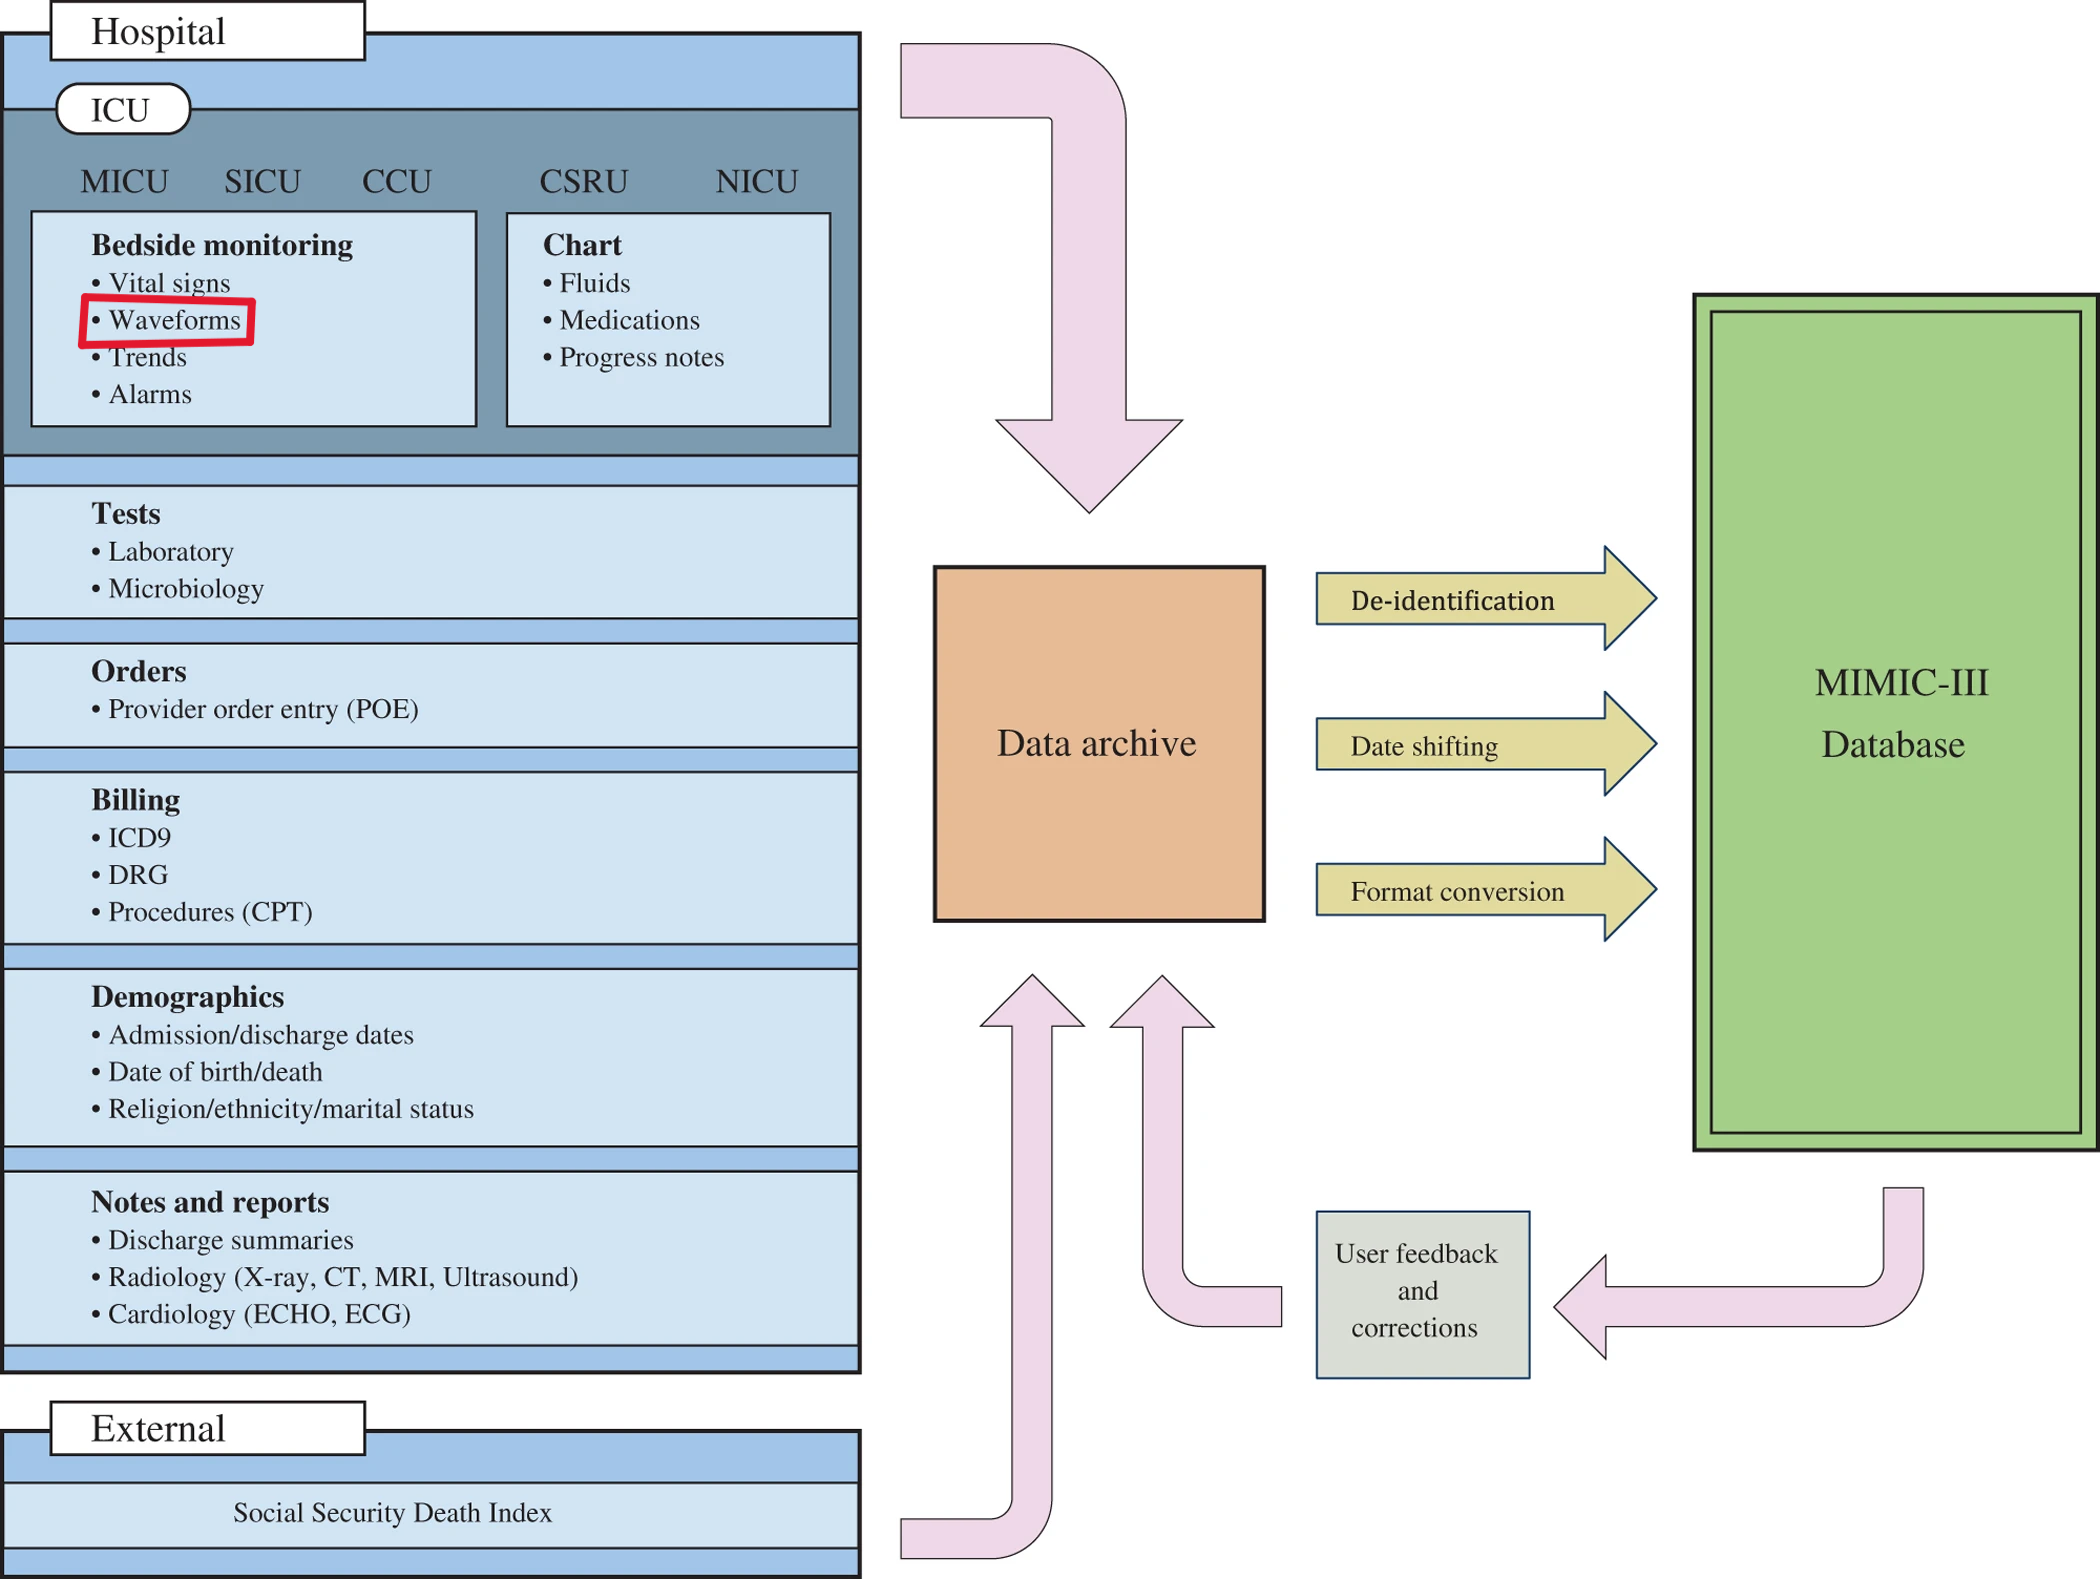
\includegraphics[scale=0.3]{images/mimic/mimic_structure}
    \caption{General Structure of the MIMIC-III DB~\cite{johnsonMIMICIIIFreelyAccessible2016}}
    \label{fig:mimic_structure}
\end{figure}

The Waveform data from both the MIMIC-III and MIMIC-IV DBs is publicly available on the Physionet internet website~\cite{moodyMIMICIIIWaveformDatabase2017, moodyMIMICIVWaveformDatabase}.
In both DBs recorded waveforms typically encompass one or more electrocardiogram(ECG) signals, often feature continuous ABP waveforms and fingertip PPG signals.
Numeric data typically includes heart and respiration rates, SpO2, and systolic, mean, and diastolic blood pressure, among other metrics when accessible.
Recording durations also vary, with most lasting a few days, although some are shorter and other might even extend over several weeks.
Both projects consist of two types of data: waveform data, comprising high-resolution, regularly sampled time series obtained directly from measuring devices, and numeric data, including digitally derived values or irregularly sampled data (like NIBP).

% Differences MIMIC3 and MIMIC4
\vspace{0.2cm}
\textit{Differences and Similarities between MIMIC-III and MIMIC-IV}
\vspace{0.2cm}

In MIMIC-III, waveforms were collected in a largely automated manner from selected adult and neonatal ICUs, resulting in a random sample of patients.
The data archiving process was not continuous, and the recorded waveforms and numerics varied based on ICU staff choices.
The individual patient consent waived due to de-identification.
On the other hand, MIMIC-IV collected data from ICUs where bedside monitors were linked to a local area network, allowing continuous monitoring and data transfer to a proprietary relational DB.
Data was stored for several weeks before being retrieved and archived daily.
The de-identification process for MIMIC-IV followed the same method as MIMIC-III, removing or replacing protected health information with non-identifying information.

Both the MIMIC-III and MIMIC-IV DBs encompass waveform and numeric datasets sourced from ICUs.
While both datasets feature detailed waveform records and numerical values, their storage and acquisition methods differ.
MIMIC-III organizes its records within a directory structure with segmented waveform data, while MIMIC-IV adopts WFDB format for waveforms and compressed CSV files for numerics.
However, MIMIC-IV incorporates enhancements like automated record partitioning and optimized storage formats to enhance data management efficiency.

% Conclusion parahraph
\vspace{0.2cm}

Clinical Research DBs such as MIMIC play a pivotal role in facilitating global access to critical patient data, thereby supporting scientific endeavors across various medical domains.
By ensuring the anonymity and de-identification of patient information, these DBs uphold stringent standards of data privacy and ethics, thereby avoiding any infringement upon patient rights or privacy regulations.
Such DBs serve as invaluable resources for conducting comprehensive studies spanning diverse medical disciplines, including but not limited to the detection and treatment of various cancers, cardiovascular diseases, and even neonatal care in stationary settings.
Their expansive datasets offer researchers an extensive pool of information to draw insights from, ultimately advancing the overall understanding and management of complex medical conditions.

\subsection{Computing Background}
\label{subsec:computing_background}

\subsubsection{Signal Processing}
\label{subsubsec:signal_processing}

This section explores various techniques and methods employed in the analysis of PPG signals and their correlation to BP measurements.
PPG-based BP estimation has emerged as a promising non-invasive approach, utilizing waveform observations from signals like PPG signals from different anatomical sites or their combination with ECG signals.
This section delves into the diverse methodologies and algorithms utilized for processing PPG signals to derive meaningful insights into BP dynamics.

% What are the methods of signal processing for reading PPG?
% Approaches for processing the given PPG data in correlation to BP
\vspace{0.2cm}
\textit{PPG Signal Processing Methods}
\vspace{0.2cm}

% PTT
Previous research has documented an inverse relationship BP and pulse transit time (PTT)~\cite{mukkamalaUbiquitousBloodPressure2015}.
Extensive investigation over past decades has focused on the PTT-based approach, revealing growing support for its potential in offering non-invasive BP measurements without the need for cuffs.
PTT refers to the delay in time for the pressure waveform to traverse between two arterial locations (see Figure~\ref{fig:ptt}).
It can be calculated as the time difference between proximal and distal waveforms indicative of the arterial pulse.
\begin{figure}[h]
    \centering
    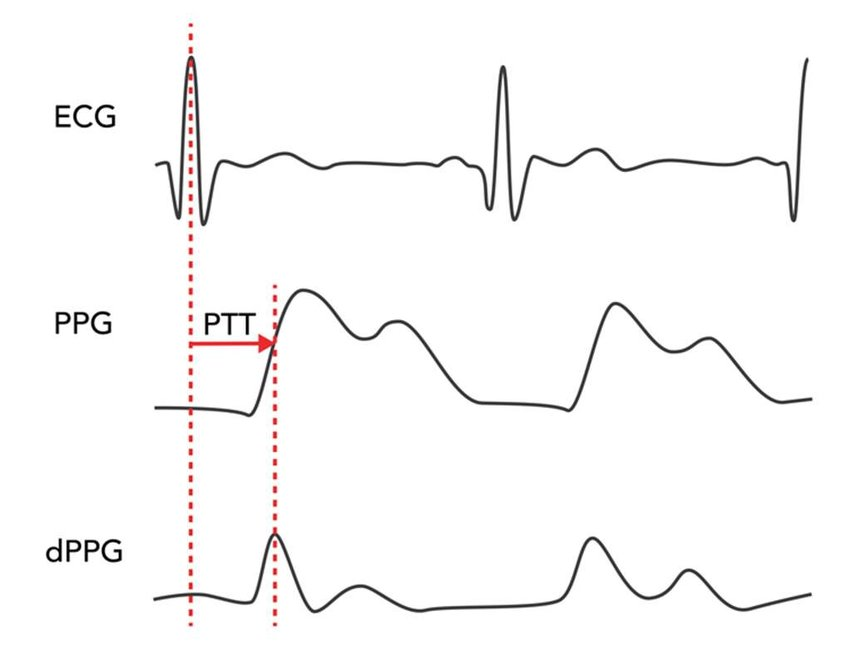
\includegraphics[scale=0.4]{images/sp/ptt}
    \caption{Calculation of PTT from ECG, PPG and first PPG derivative waveforms~\cite{luiNovelCalibrationProcedure2018}}
    \label{fig:ptt}
\end{figure}

% PAT
Pulse arrival time (PAT) represents another widely employed technique~\cite{sharmaCuffLessContinuousBlood2017}.
It is defined as the time that takes the pulse wave to travel from the heart to a peripheral site e.g.\ finger, toe, etc.
It denotes the temporal discrepancy between the R-peak of the ECG signal and the peak of the PPG signal, measured within the same cardiac cycle (see Figure~\ref{fig:pat}).
Both PTT and PAT require simultaneous measurement at two different sites on the body, hence two measurement sensors (ECG and PPG) are needed for recording the signals in order to estimate these parameters.
\begin{figure}[h]
    \centering
    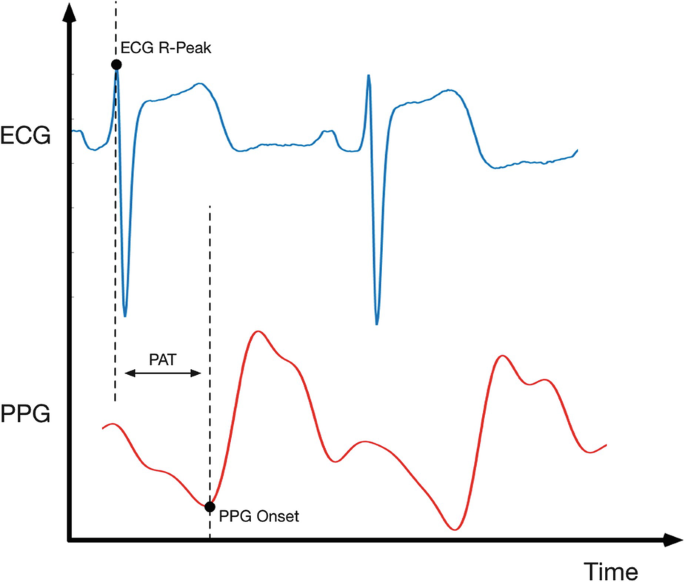
\includegraphics[scale=0.4]{images/sp/pat}
    \caption{Calculation of PAT from ECG and PPG waveforms~\cite{dhillonPulseArrivalTime2019}}
    \label{fig:pat}
\end{figure}

% PWV
Pulse wave velocity (PWV) is another alternative method for estimating BP~\cite{mccombieAdaptiveBloodPressure2006}.
PWV determines the speed of the pulse wave by utilizing two PPG sensors positioned along the same arterial branch, separated by a known distance (see Figure~\ref{fig:pww}), portrayed by the following formula
\begin{math}
    PWW = \frac{D}{PTT}
\end{math}
where D is the distance between two known body parts.

\begin{figure}
    \begin{minipage}[c]{0.5\textwidth}
        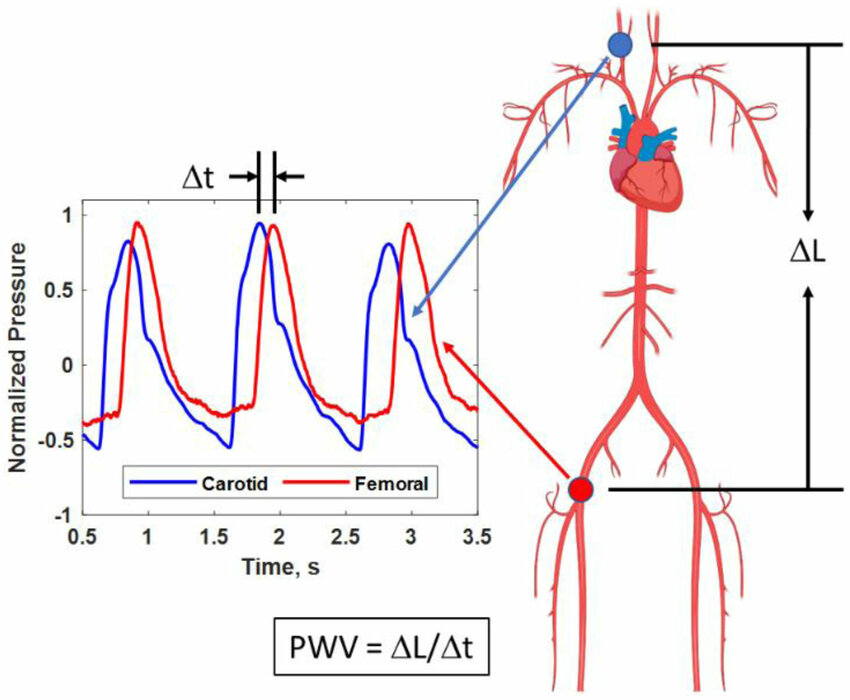
\includegraphics[width=\textwidth]{images/sp/pww}
    \end{minipage}\hfill
    \begin{minipage}[c]{0.5\textwidth}
        \captionsetup{format=plain, justification=centering}
        \caption{Calculation of PWW from two PPG signals at different body parts~\cite{urbanUnderstandingArterialBiomechanics2023}}
        \label{fig:pww}
    \end{minipage}
\end{figure}

% summarize PTT,PAT,PWV
Estimating BP through PTT, PAT, or PWV parameters involves mathematical models, but implementing these models faces challenges, and none of these techniques has become a reliable clinical tool for BP measurement.
Challenges include the need for synchronized sensors, varying sampling rates, and reliance on complex arterial wave propagation models, making continuous BP measurement inconvenient and requiring constant calibration.
Despite per-person calibration, these models offer only short-term BP estimation and remain unreliable for beat-to-beat BP measurement.

% PWA
Pulse wave analysis (PWA) offers a multifaceted solution to the previously mentioned issues.
It serves as an umbrella term encompassing signal processing and feature extraction of certain PPG waveform characteristics.
PWA offers a novel method for cuffless, continuous, and calibration-free BP measurement by extracting temporal features from the PPG waveform, which demonstrate a strong correlation with individual BP levels~\cite{elgendiAnalysisFingertipPhotoplethysmogram2012}.
Utilizing only one PPG sensor, PWA presents several advantages over previous methods, including simplicity, affordability, straightforward signal acquisition, and a resemblance between BP pulse waveform and PPG blood volume pulse (example in Figure~\ref{fig:pwa}).
This data-driven approach to BP estimation provides optical BP measurement with promising potential for practical applications.
Advancements in computational technology and data analysis software have simplified the preprocessing and analysis of physiological signals.
Techniques such as filtering and feature extraction are commonly utilized in the analysis of PPG pulse waves, often integrated into ML and deep neural network (DNN) models for blood pressure estimation.
\begin{figure}[h]
    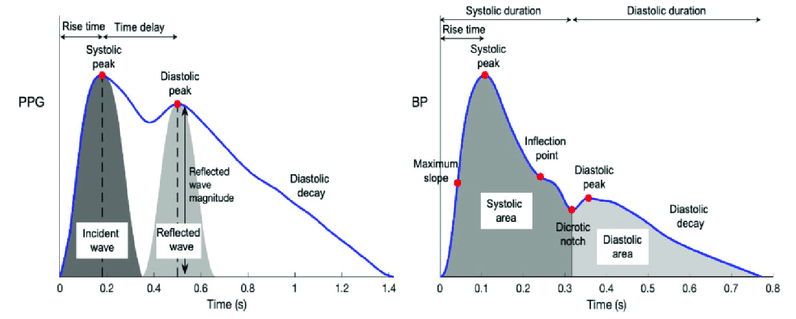
\includegraphics[width=\textwidth]{images/sp/pwa}
    \caption{Example of a PWA used to extract features from the PPG waveform~\cite{bikiaLeveragingPotentialMachine2021}}
    \label{fig:pwa}
\end{figure}

% Different types of filters for processing the PPG signal
\vspace{0.2cm}
\textit{Signal Pre-Processing}
\vspace{0.2cm}

The preprocessing of physiological signals, crucial for accurate BP estimation, involves a variety of signal filtering techniques.
Techniques like Chebyshev, Butterworth, and Savitzky-Golay filtering, along with methods such as second derivative analysis, play pivotal roles in enhancing signal quality.
These preprocessing steps, facilitated by advancements in computational technology, pave the way for more refined analysis and interpretation of PPG pulse waves.

% Butterworth
An investigation into various signal pre-processing techniques necessitates an examination of different types of filters.
One prominent representative is the Butterworth filter, characterized by its flat frequency response within the passband.
Belonging to the Infinite Impulse Response (IIR) category, Butterworth filters offer efficiency in processing low-frequency signals and exhibit rapid computational capabilities, as demonstrated by Chatterjee et al.\ in their PPG-based heart rate analysis~\cite{chatterjeePPGBasedHeart2018}.
The filter order directly correlates with the number of energy storage components present in the analogous analog circuit, such as inductors and capacitors.
The transfer function of a Butterworth filter is represented by the following formula, where \texttt{n} is the filter order and \texttt{z} is the complex variable used in Z-transform analysis:
\Large
\begin{center}
    \begin{math}
        H(z) = \frac{1}{[1 + (z^{-1})^{n}]^{1/2}}
    \end{math}
\end{center}
\normalsize

% SavGol
Another noteworthy filter type is the Savitzky-Golay filter, introduced by Savitzky and Golay~\cite{savitzkySmoothingDifferentiationData1964}.
Falling under the Finite Impulse Response (FIR) category, this filter effectively smooths data while removing unwanted frequencies.
Its inherent stability ensures a finite output for any finite input.
Additionally, the linear phase property guarantees the absence of frequency-dependent time shifts.
The Savitzky-Golay filter doesn't have a single transfer function like the Butterworth filter because it belongs to the FIR category.
Instead, it relies on convolution with pre-calculated coefficients specific to the desired characteristics.
The filter fits a low-degree polynomial to a window of data points around each point in the signal.
The smoothed value is then the value of the fitted polynomial at the center point.
Different polynomial degrees and window sizes lead to different filtering effects.
The relationship can be expressed by the following formula:
%\Large
%\begin{center}
%    \begin{math}
%        y[n]~=~\sum_{i=-\frac{M}{2}}^{\frac{M}{2}} W_i~\cdot~x_{n+i} \\
%        \normalsize
%        \begin{array}{ll}
%            M       & : \text{Window size (odd number greater than or equal to N+1)} \\
%            N       & : \text{Polynomial degree}                                     \\
%            W_i     & : \text{Filter coefficients (length M)}                        \\
%            x_{n+i} & : \text{Signal data point}                                     \\
%            y[n]    & : \text{Smoothed data point}
%        \end{array}
%    \end{math}
%\end{center}
%\normalsize

% Chebyshev
Furthermore, the Chebyshev filter offers a steeper roll-off compared to other filters, leading to sharper distinctions between desired and unwanted frequencies.
While this advantage comes at the cost of controlled passband ripples, these filters remain valuable tools for applications requiring precise frequency separation.
Beyond digital signal improvement, they find applications in audio crossovers, image noise reduction, and data communication, as discussed by Antoniou~\cite{antoniouDigitalFiltersAnalysis2018}.
While the Chebyshev filter has a transfer function like the Butterworth filter, it's slightly more complex due to its specific characteristics.
Unlike the Savitzky-Golay filter, its coefficients depend on the desired ripple level and order, making a single, universal formula impractical.
The general form of the Chebyshev filter transfer function depends on whether it's Type I (equiripple in both passband and stopband) or Type II (equiripple only in the stopband).
The corresponding functions are presented by the following formulas:~
%\begin{multicols}{2}
%    \begin{center}
%        Chebyshev I \\
%        \vspace{0.2cm}
%        \large
%        \begin{math}
%            H(z) = K \prod_{n=1}^{N} \left[ 1 - \frac{\varepsilon}{(T_n(z))^2} \right]
%        \end{math}
%        \normalsize
%        \begin{tabular}{ll}
%            $K$           & : Gain factor                 \\
%            $\varepsilon$ & : Normalized passband         \\           & \;\, ripple level (dB)                \\
%            $N$      & : Filter order \\
%            $T_n(z)$      & : Chebyshev polynomial of the \\      & \;\, first kind, evaluated at $z$ \\
%        \end{tabular}
%    \end{center}
%    \columnbreak
%    \begin{center}
%        Chebyshev II \\
%        \vspace{0.2cm}
%        \large
%        \begin{math}
%            H(z) = K \cdot \frac{z^N - 1}{\prod_{n=1}^{N} \left[ z^2 - 2 \zeta z \cos(\omega_n) + 1 \right]}
%        \end{math}
%        \normalsize
%        \begin{tabular}{ll}
%            $K$        & : Gain factor                        \\
%            $N$        & : Filter order                       \\
%            $\zeta$    & : Normalized stopband damping factor \\
%            $\omega_n$ & : Normalized cutoff frequency        \\
%        \end{tabular}
%    \end{center}
%\end{multicols}

% Optimal finding
In their 2018 study, Liang et al.\ investigated nine different digital signal filters to identify the optimal approach for short PPG signals (2.1s)~\cite{liangOptimalFilterShort2018}.
Some of the filters included the Butterworth, Elliptical, Chebyshev Type I and II, Median Filter etc.
Their performance-based ranking revealed the Chebyshev II filter as the most effective in enhancing PPG signal quality, with the optimal order at 4th.

% miscallaneous sp approaches
\vspace{0.2cm}
\textit{Miscellaneous Signal Processing Approaches}
\vspace{0.2cm}

A study conducted by Takazawa et al.\ investigated the utilization of the second derivative of the fingertip PPG waveform within clinical contexts~\cite{takazawaAssessmentVasoactiveAgents1998}.
The research analysed changes in patients' pressure, wave ratios, age-related variations, and correlations with health conditions.
Collectively, the results indicate the potential value of the second derivative in appraising the impacts of specific medications and assessing vascular health and aging, offering potential avenues in arteriosclerotic disease screening.
Subsequent research has demonstrated the effective application of the second derivative of the PPG waveform in identifying the dicrotic notch within a single pulse wave (see Figure~\ref{fig:dic_notch}), a critical landmark in PWA\@.

\begin{figure}[h]
    \centering
    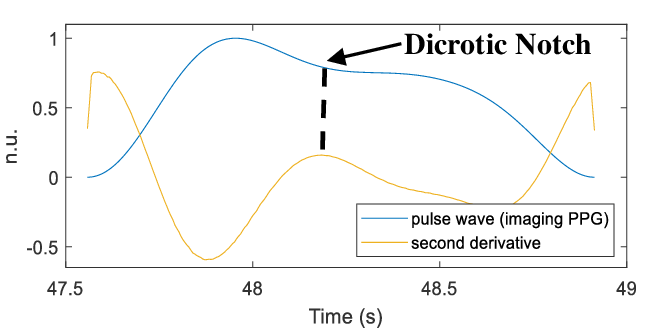
\includegraphics[scale=0.6]{images/sp/dic_notch}
    \caption{Dicrotic Notch Approximation from the Second Derivate of the PPG~\cite{djeldjliImagingPhotoplethysmographySignal2019}}
    \label{fig:dic_notch}
\end{figure}

In 2022, Charlton et al.\ conducted a collaborative study to investigate the hemodynamic characteristics of photoplethysmogram (PPG) waveforms for the purpose of vascular age assessment~\cite{charltonAssessingHemodynamicsPhotoplethysmogram2022}. A key outcome of their work was the identification of a comprehensive set of features, termed "fiducial points," which could be extracted from the PPG waveform to achieve accurate vascular age estimation.

The term \enquote{fiducial} originates from the Latin \textit{fiducialis}, meaning \enquote{reliable}.
In the context of signal processing, it refers to reference points employed for precise measurements.
In the early cases, it has been used for accurate determination of pulse transit time (PTT) between the R-wave of the electrocardiogram (ECG) and a designated point in a finger PPG pulse, as demonstrated by Zhang et al.~\cite{zhangEffectLocalCold2005}.
In the study by Charlton et al., these points were repurposed to delineate diverse landmarks (identified as Row A in Figure~\ref{fig:fiducials}) on the pulse wave, serving as references for extracting both temporal and amplitude-based features.

\begin{figure}[h]
    \centering
    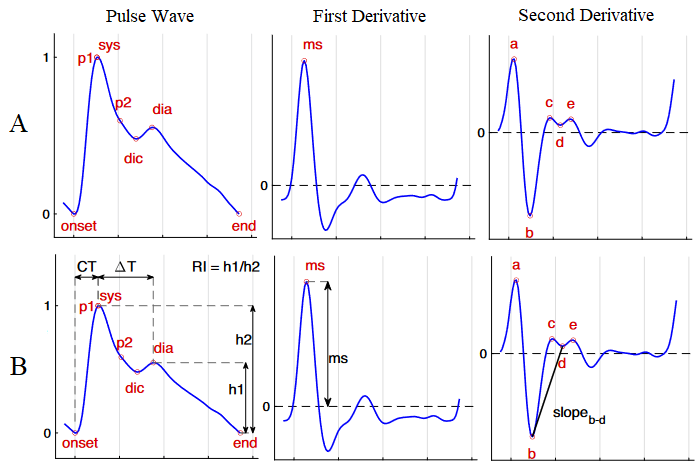
\includegraphics[scale=0.8]{images/sp/fiducials}
    \caption{A - Fiducial Point Identification; B - Feature Calculation~\cite{charltonAssessingHemodynamicsPhotoplethysmogram2022}}
    \label{fig:fiducials}
\end{figure}

Building upon the identified fiducial points, Charlton et al.\ employed various techniques to extract meaningful values from a single PPG signal (Row B in Figure~\ref{fig:fiducials}) that contribute to vascular age assessment.
This section provides a summary of the implemented methods and corresponding example values (presented in brackets):
\begin{enumerate}
    \item Pulse Wave Features (crest time: time from \texttt{onset} to \texttt{sys})
    \item First Derivative Features (minimum rise time: amplitude of pulse wave divided by amplitude of \texttt{ms})
    \item Second Derivative Features (aging index: defined as amplitude values of \mbox{\texttt{(b-c-d-e)/a)}}
    \item Combination of Features (minimum rise time: \texttt{[1/x0(ms)]·[x(sys) - x(onset)]})
    \item Frequency Domain Analysis (Fast Fourier Transform (FFT) analysis: Use of FFT to extract amplitude and phase information from the PPG signal)
    \item Features From Multiple Beats (pulse rate variability parameters)
\end{enumerate}

\vspace{0.2cm}
This section explored diverse signal processing techniques.
As mentioned previously, traditional methods relying on physiological parameters (PAT, PTT, PWV) face limitations.
Signal processing approaches like PWA, filtering, and feature extraction are often integrated with ML models and provide a higher BP detection accuracy.
These approaches show promising results for cuffless, continuous BP estimation using PPG signals, paving the way for practical non-invasive BP monitoring solutions.

\subsubsection{Machine Learning}
\label{subsubsec:machine_learning}

Building upon the foundation laid by traditional signal processing techniques, ML emerges as a transformative force in the pursuit of accurate and non-invasive BP estimation using PPG signals.
This section delves into the diverse tapestry of ML methods currently employed, thoroughly exploring their individual approaches and their collective potential to improve cuffless BP monitoring.

\begin{figure}[h]
    \centering
    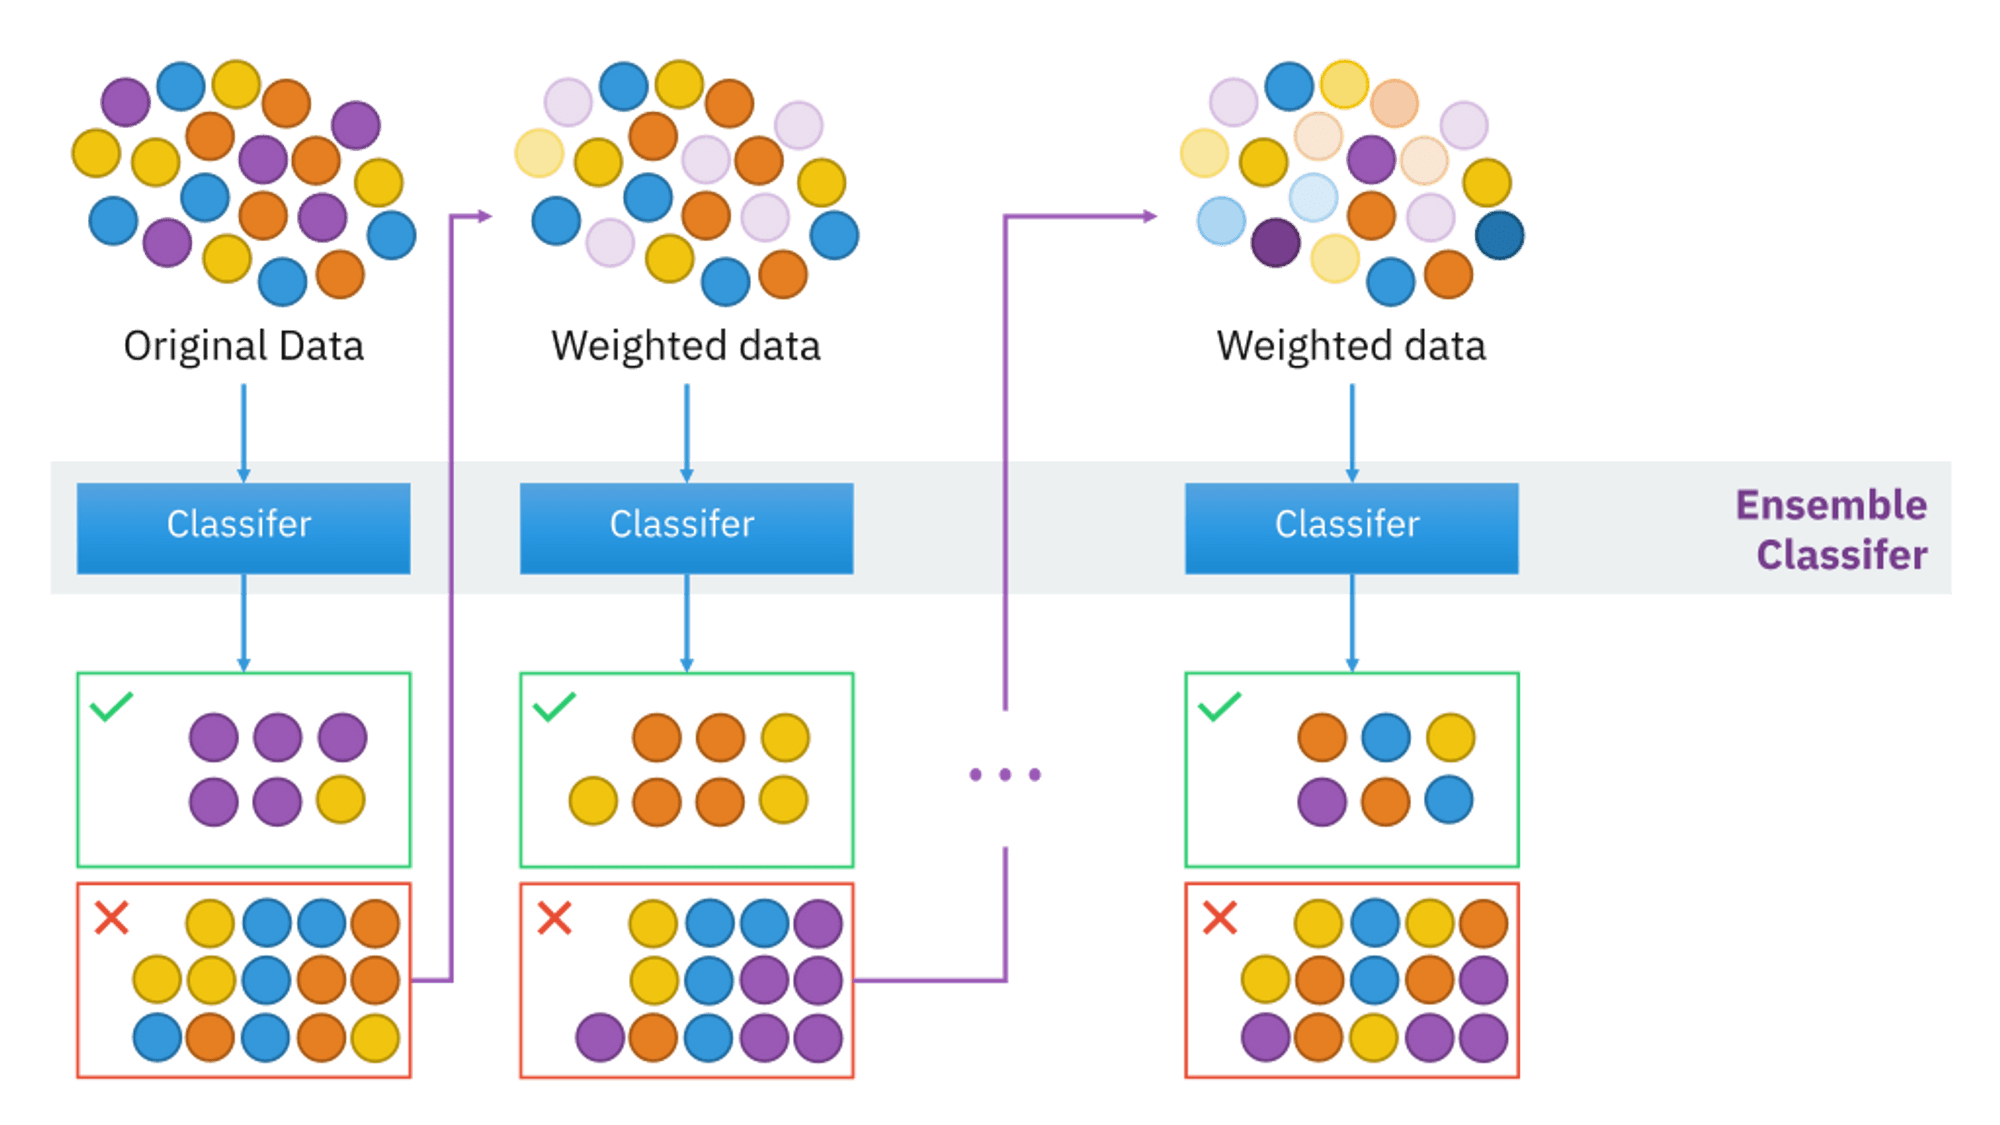
\includegraphics[scale=0.06]{images/ml/adaboost}
    \caption{\small AdaBoost, or Adaptive Boosting, is an ensemble learning technique that iteratively combines weak classifiers to create a strong classifier by adjusting weights based on classification errors~\cite{AdaBoostAlgorithmMachine}}
    \label{fig:adaboost}
\end{figure}

% ML Techniques
\vspace{0.2cm}
\textit{Machine Learning Approaches}
\vspace{0.2cm}

BP estimation using ML techniques is data driven, unlike the traditional PTT/PAT only models.
Several studies attempted to fit regression models, such as multilinear regression, support vector machine (SVM) and random forest, for estimating BP using PTT/PAT based approach with some degree of success, but the results did not always satisfy the international standards.

As early as 2003, Teng and Zhang~\cite{tengContinuousNoninvasiveEstimation2003} were among the pioneers in exploring non-invasive methods for estimating blood pressure without the need for traditional cuff-based techniques.
They explored the relationship between four PPG features and BP using a linear regression (LR) model.
While diastolic time exhibited the strongest correlation with both SBP and DBP, the overall results suggested limitations in LR for accurate BP estimation.

Recognizing these limitations, Suzuki and Oguri (2009) introduced AdaBoost (example in Figure~\ref{fig:adaboost}), a classifier, for SBP estimation~\cite{suzukiCufflessBloodPressure2009}.
This methodology segmented SBP values using a threshold before employing a nonlinear ML model, showcasing the need for more complex techniques.

Seeking a different approach, Ruiz-Rodriguez et al.\ (2013) utilized a Deep Belief Network Restricted Boltzmann Machine (RBM) for simultaneous prediction of SBP, DBP, and MAP~\cite{ruiz-rodriguezInnovativeContinuousNoninvasive2013a}.
An example DBN and RBM with custom input and output sizes is illustrated in Figure~\ref{fig:rbm}
However, the study yielded highly variable results, raising concerns about its reliability.

\begin{figure}[h]
    \centering
    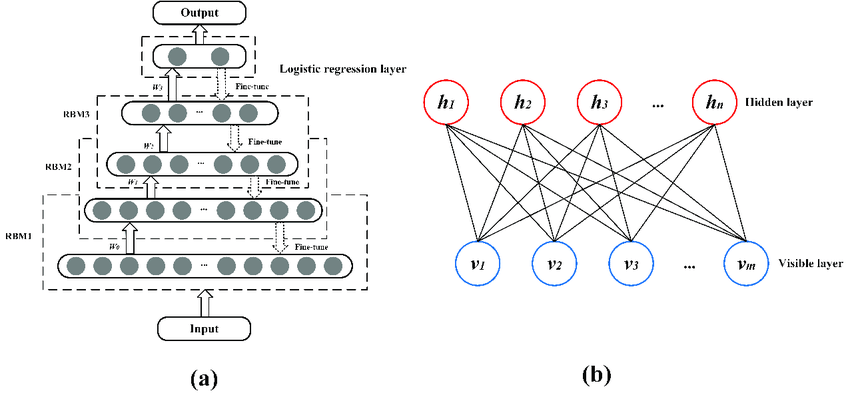
\includegraphics[scale=0.5]{images/ml/RBM}
    \caption{\small A DBN (a) combines multiple layers of RBMs (b) to form a generative model capable of learning hierarchical representations of the data~\cite{ouIntegratingCellularAutomata2019}}
    \label{fig:rbm}
\end{figure}

Shifting focus to feature extraction, Kurylyak et al.\ (2013) extracted 21 features from the PPG waveform and used a feedforward NN (example in Figure~\ref{fig:ffnn}) for SBP and DBP estimation~\cite{kurylyakNeuralNetworkbasedMethod2013}.
Their promising results demonstrated the potential of NN-based approaches.

\begin{figure}[h]
    \centering
    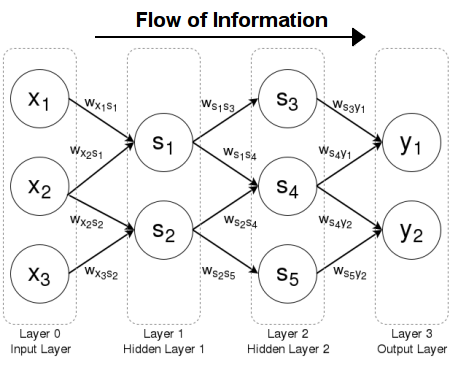
\includegraphics[scale=0.5]{images/ml/ffnn}
    \caption{\small Feed Forward NNs have connections between the nodes that do not form cycles, allowing data to move in only one direction, from the input nodes through the hidden nodes to the output nodes, with each connection having an associated weight~\cite{FeedforwardNeuralNetworks}}.
    \label{fig:ffnn}
\end{figure}

Xing and Sun (2016) ventured into the frequency domain, applying Fast Fourier Transformation to select features followed by a feedforward NN for BP estimation~\cite{xingOpticalBloodPressure2016}.
While initial results were encouraging, the authors recognized the need for broader feature space exploration.

Building upon Kurylyak et al.'s work, Liu et al.\ (2017) incorporated 14 second derivative features and employed an SVM for BP estimation, highlighting the value of diverse feature extraction techniques~\cite{liuIntegratedNavigationTethered2017}.

Marking a significant shift, Su et al.\ (2018) explored a four-layer bidirectional Long Short-term memory (LSTM) model with residual connections, demonstrating the promise of recurrent NNs~\cite{suLongtermBloodPressure2018}.
The working principle of an LSTM is demonstrated in Figure~\ref{fig:lstm}.

\begin{figure}[h]
    \centering
    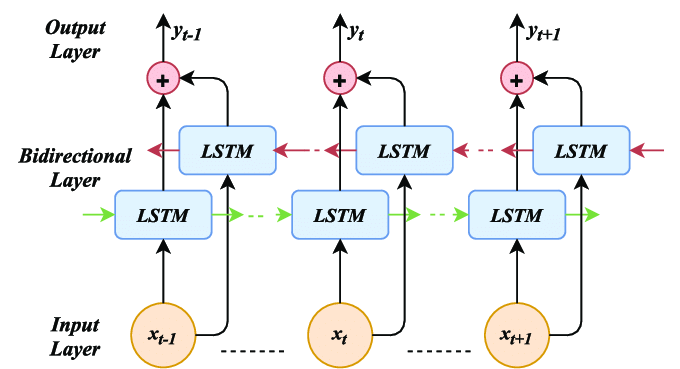
\includegraphics[scale=0.5]{images/ml/lstm}
    \caption{\small Bidirectional LSTM is a type of recurrent neural network architecture that processes sequential data in both forward and backward directions. This allows the model to capture dependencies from past and future contexts simultaneously, enhancing its ability to understand and predict patterns in sequential data~\cite{anishnamaUnderstandingBidirectionalLSTM2023}}.
    \label{fig:lstm}
\end{figure}

A 2019 study by Tanveer and Hasan introduced a hierarchical Artificial NN-LSTM model for blood pressure estimation, comprising two levels: the lower level employed ANNs to extract morphological features from ECG and PPG waveforms, while the upper level utilized LSTM layers to address temporal variations in these features~\cite{tanveerCufflessBloodPressure2019}.
They also found, that DBP is strongly associated with SBP and can enhance its estimation, suggesting simultaneous modeling using a single architecture for both.

Focusing on long term estimation, El-Hajj and Kyriacou (2021) proposed leveraging advanced deep learning techniques like Bidirectional-LSTMs and Bidirectional Gated Recurrent Units (GRU) with attention mechanisms (example of attention mechanism implementation in LSTM in Figure~\ref{fig:attention}) for BP estimation~\cite{el-hajjDeepLearningModels2021}.

\begin{figure}
    \begin{minipage}[c]{0.5\textwidth}
        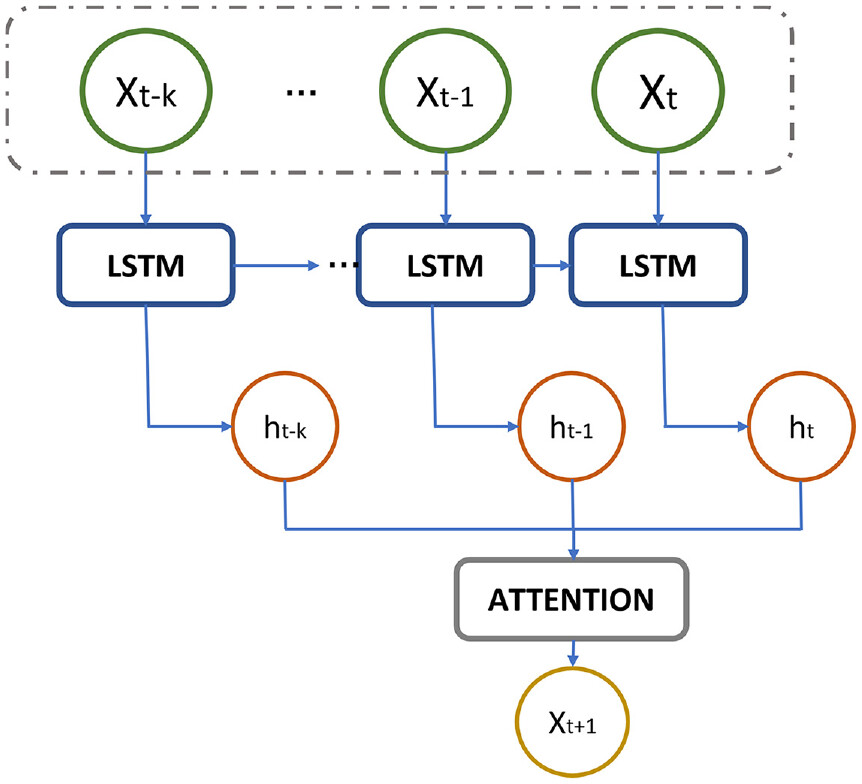
\includegraphics[width=\textwidth]{images/ml/attention}
    \end{minipage}\hfill
    \begin{minipage}[c]{0.5\textwidth}
        \captionsetup{format=plain, justification=centering}
        \caption{\small The attention mechanism in LSTM allows the model to focus on specific parts of the input sequence, dynamically adjusting the importance of each input element during the prediction process~\cite{marulandaHybridModelBased2023}}
        \label{fig:attention}
    \end{minipage}
\end{figure}

%\begin{figure}
%\floatbox[{\capbeside\thisfloatsetup{capbesideposition={right,top},capbesidewidth=4cm}}]{figure}[\FBwidth]
%{\caption{A test figure with its caption side by side}\label{fig:at}}
%{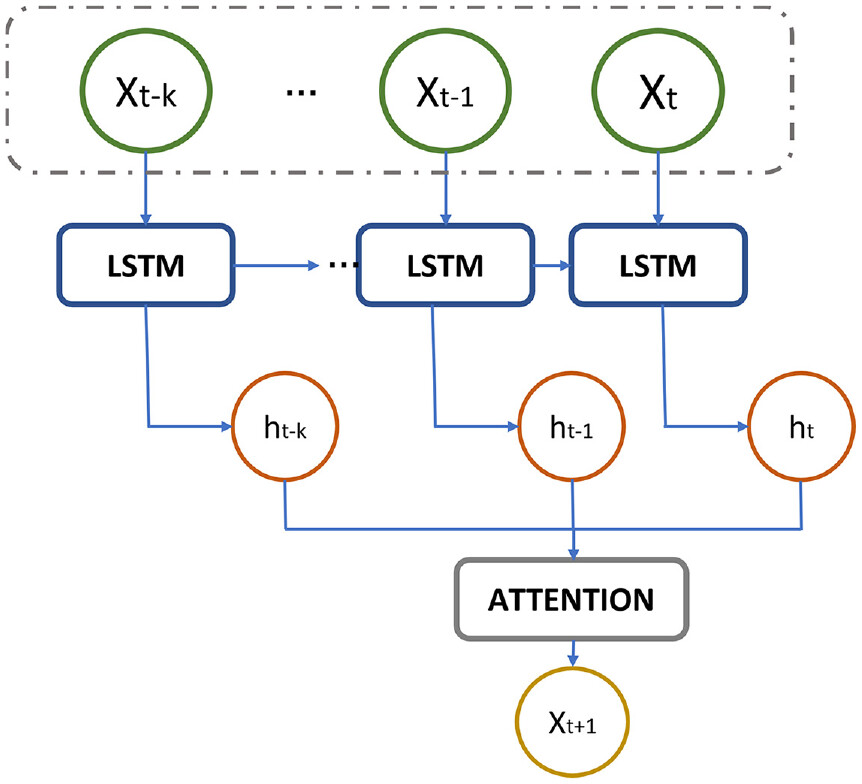
\includegraphics[scale=0.5]{images/ml/attention}}
%\end{figure}

Recognizing the need for real-world applicability, Joung et al.\ (2023) evaluated a learning-driven cuffless BP estimation system under challenging conditions with calibration~\cite{joungContinuousCufflessBlood2023}.
Their 1D convolutional NN highlighted the importance of addressing various real-world scenarios.

These early studies illustrate the evolution of ML techniques for cuffless BP estimation, paving the way for further advancements.
From exploring linear relationships to harnessing the power of deep learning, researchers continue to refine and develop novel approaches.
While challenges remain, these pioneering efforts demonstrate the immense potential of ML in improving non-invasive BP monitoring, and future research holds the promise for even more accurate and robust solutions.

\vspace{0.2cm}

To conclude, the relationship between PPG characteristics and BP was not found to consistently follow a linear trend.
Conventional linear models frequently struggle to effectively capture the complex relationship between BP and PPG when analysed across various demographic datasets.
Traditional ML algorithms like SVMs and Random Forest tend to achieve higher accuracy rates in this context.
To estimate BP accurately using these techniques, distinct models are typically constructed for SBP and DBP\@.
However, recent evidence suggests that a unified architecture capable of simultaneously modeling SBP, DBP, and even MAP is both feasible and advantageous.
Various advanced NN models demonstrate superior efficiency in integrating such architectures and leveraging extensive datasets with heightened precision relative to conventional ML approaches.


    \section{Methods}
    \label{sec:methods}
    The Methods section provides an overview of the methodologies employed in the \texttt{PPG-BP} project.
It encompasses various subdirectories such as MIMIC and PyTorch tutorials, with the primary code located within the \texttt{model} Python Package.
Within the \texttt{model}, there exist several sub-packages containing relevant data for subsequent project components,
while the core code is distributed across five \texttt{.py} classes: \texttt{init\_scripts.py} (Initialization / Data Fetching), \texttt{sp\_scripts.py} (Signal Processing),
\texttt{ml\_scripts.py} (Machine Learning), \texttt{visual.py} (Visualization), and \texttt{main.py}, which integrates all the aforementioned components.
The whole repository can be found on the author's \textit{GitHub} page~\cite{jasinskasHtjasPPGBPProject2024}.

\subsection{Data Fetching}
\label{subsec:data-fetching}

The initial phase in virtually all Data Science endeavors involves Data Preparation.
This section will examine the \texttt{init\_scripts.py} class.
For this project, data was sourced from the MIMIC-III and MIMIC-IV DBs, each serving distinct purposes.
Data from the MIMIC-IV DB was employed as the validation dataset (detailed further in the ML methods section~\ref{subsec:ml_methods}), since it is regarded as the most modern and most reliable MIMIC DB currently available.
In contrast, data from the MIMIC-III database was utilized for training and testing ML models due to its significantly larger size.
Nevertheless, the data retrieval process employed similar methods for both the older and newer waveform datasets.

% Libraries
\vspace{0.2cm}
\textit{Tools and Approaches}
\vspace{0.2cm}

Researchers at the MIT Laboratory for Computational Physiology have developed a native Python library named the waveform-database (WFDB) package, facilitating the convenient handling of MIMIC datasets.
This library comprises tools for reading, writing, and processing WFDB signals and annotations~\cite{MITLCPWfdbpython2024}.
Efficient and consistent data retrieval was achieved through a combination of pre-existing WFDB library functions and custom-written methods.

First of all, a list of all records from the selected DB were fetched utilizing the

\vspace{0.1cm}
{\centering \texttt{wfdb.get\_record\_list(db\_name)}\par}
\vspace{0.1cm}

\noindent method.
Then an iterative process followed, going through all the subjects from the loaded records list.
When assessing a single subject, the same method, but with more specific parameters

\vspace{0.1cm}
{\centering \texttt{wfdb.get\_record\_list((f'{db\_name}/{subject}')}\par}
\vspace{0.1cm}

\noindent was called, in this instance to load all studies from a single subject.
Another loop was formed to iterate through each study within the subject.
These studies consist of records, each representing a single ICU \enquote{session}, during which the patient was connected to at least one monitoring device, therefore they highly differ in time length.
Given the diversity of monitoring devices, these records encompass various signals, including ECG, ABP, and Pleth (equivalent to PPG).
To verify if the record includes all the required signals (ABP and Pleth for this study), the method

\vspace{0.1cm}
{\centering \texttt{record\_data = wfdb.rdheader(subject.name, record\_dir, rd\_segments=True)}\par}
\vspace{0.1cm}

\noindent was invoked, providing the header data of a single record, which is then used to fetch all present signals

\vspace{0.1cm}
{\centering \texttt{signal\_names = record\_data.sig\_name}.\par}
\vspace{0.1cm}

\noindent If the record lacks either the \textit{ABP} or \textit{Pleth} signals, it is excluded from further processing.
However, even a single record comprises multiple segments, varying in duration and the signals they capture.
If a record lacks either the ABP or Pleth signals, it is excluded from further processing.
Each record comprises multiple segments, varying in duration and the signals they capture.
In addition to signal requirements, segments must also have a minimum length of 10 minutes to be considered usable.
This criterion aims to ensure data reliability and variability, as longer segments offer more data points to represent physiological states accurately, reducing the impact of short-term fluctuations and noise.
The segment duration length is determined by the following function:

\vspace{0.1cm}
\qquad\qquad\qquad \texttt{segment\_metadata = wfdb.rdheader(segment, record\_dir)}

\qquad\qquad\qquad \texttt{tot\_seg\_length = segment\_metadata.sig\_len}

\qquad\qquad\qquad \texttt{sampling\_rate = segment\_metadata.fs}

\qquad\qquad\qquad \texttt{seg\_duration = tot\_seg\_length / fs}
\vspace{0.1cm}

\noindent Precisely these segments represent the smallest data samples utilized in this study, containing continuous numeric values sampled at a specific frequency rate.
The data abstraction levels in MIMIC DBs can be depicted by the chart, showing a descending order from left to right:

\vspace{0.1cm}
{\centering \textit{Subject} $\rightarrow$ Study $\rightarrow$ Record $\rightarrow$ Segment\par}
\vspace{0.1cm}

An iterative process is likewise applied to every segment of a record, by fetching all values from a single segment:

\vspace{0.1cm}
{\centering \texttt{segment\_data = wfdb.rdrecord(segment, record\_dir)}.\par}
\vspace{0.1cm}

\noindent These segments should also be devoid of any \enquote{faulty} values, identified as NumPy values \texttt{NaN} and \texttt{inf}.
For ABP segments values outside the range of 30 to 250 (accounting for extreme and likely erroneous measurements) are omitted, and for Pleth values must strictly fall between 0 and 1 (representing the valid PPG range).
These exclusion criteria are summarized in Table~\ref{tab:faulty}.

\begin{wraptable}{r}{0.35\textwidth}
    \begin{center}
        \begin{tabular}{ |c|c| }
            \hline
            ABP              & Pleth         \\
            \hline
            30 $<$ x $<$ 250 & 0 $<$ x $<$ 1 \\
            \hline
            \multicolumn{2}{|c|}{not \texttt{NaN}, \texttt{inf}} \\
            \hline
        \end{tabular}
    \end{center}
    \vspace*{-7mm}
    \captionsetup{format=plain, justification=centering}
    \caption{\small Criteria for non-faulty values in data fetching}
    \label{tab:faulty}
\end{wraptable}

If a 10-minute continuous part of the segment matches these criteria, it is saved to the \texttt{./mimic3} (or \texttt{./mimic4}) directory, as 2 separate and synchronous ABP and PPG files.
If a segment is longer than 10 minutes, then more 10 minute segments may be extracted (marked by a \_ and a number representing the \textit{n-th} 10 minute part of a segment)
Examples of the file names and their values are illustrated in Figures~\ref{fig:segments} and~\ref{fig:values}.

\begin{wrapfigure}{r}{0.35\textwidth}
    \vspace*{-10mm}
    \begin{center}
        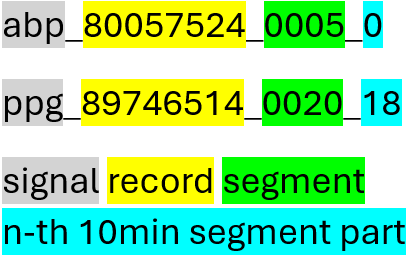
\includegraphics[width=0.3\textwidth]{images/methods/segments}
    \end{center}
    \vspace*{-7mm}
    \captionsetup{format=plain, justification=centering}
    \caption{\small Examples of extracted segment files}
    \label{fig:segments}
\end{wrapfigure}

As noted earlier, each subject in the database may encompass multiple studies, records, and segments.
To prevent disproportionate representation of individual patient data, a limit of 100 segments, each spanning 10 minutes, was imposed per subject.
This is specifically important for data retrieval from the MIMIC-III database, which is intended for training and testing purposes.
However, this restriction was not applied to data retrieval from the MIMIC-IV database, which is designated for validation purposes and aims to encompass all available 10-minute segments, thus simulating real-world data where over-representation is not a concern.

\begin{wrapfigure}{r}{0.35\textwidth}
    \vspace*{-5mm}
    \begin{center}
        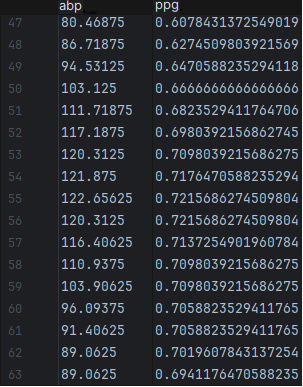
\includegraphics[width=0.3\textwidth]{images/methods/values}
    \end{center}
    \vspace*{-7mm}
    \captionsetup{format=plain, justification=centering}
    \caption{\small Example raw ABP and PPG values}
    \label{fig:values}
\end{wrapfigure}

Additionally, the primary objective was to achieve a dataset split ratio of 60/20/20 for training, testing, and validation, where 80\% of the data comprises the MIMIC-III dataset for training and testing (60/20), and the remaining 20\% consists of the MIMIC-IV dataset for validation purposes.
To facilitate this, an initial set of x segments was retrieved from the MIMIC-IV database, followed by obtaining four times the number of x segments from the MIMIC-III database.
However, it is important to acknowledge that the quantity of segments obtained from each database doesn't directly correspond to the number of features utilized in the ML phase, as signal processing (SP) tasks are performed in between.
Thus, the 60/20/20 split ratio for training, testing, and validation serves more as a guideline than an absolute target for the number of segments retrieved.
Details on achieving the actual proportions are provided in the subsequent section~\ref{subsec:sp_methods}.

\subsection{Signal Processing}
\label{subsec:sp_methods}

After the initial Data Preparation phase, the Signal Processing follows.
Its code is written in the \texttt{sp\_scripts.py} file.
The main \texttt{process\_data()} method is made up of these 6 steps (description and corresponding Python code):
\begin{enumerate}
    \item reading the fetched waveform data, \newline
    \small \texttt{seg\_name,raw\_abp,raw\_ppg = read\_seg\_data(filename,bp\_path,ppg\_path,fs)}
    \item \normalsize preprocessing the data, \newline
    \small \texttt{abp\_filt,ppg\_filt = pre\_process\_data(raw\_abp,raw\_ppg,fs,seg\_name)}
    \item \normalsize determining beats and heart rate (HR), \newline
    \small \texttt{abp,ppg,abp\_beats,ppg\_beats = signal\_processing(seg\_name,abp\_filt,ppg\_filt,fs)}
    \item \normalsize identifying fiducial points, \newline
    \small \texttt{abp\_fidp = fiducial\_points(abp,abp\_beats, fs) \newline ppg\_fidp = fiducial\_points(ppg, ppg\_beats, fs)}
    \item \normalsize extracting relevant features, \newline
    \small \texttt{features = extract\_features(abp\_fidp,ppg\_fidp,abp,ppg,fs,median\_window)}
    \item \normalsize saving extracted features. \newline
    \small \texttt{save\_split\_features(tot\_abp\_values,median\_abp\_values,tot\_ppg\_values,median\_ppg\_values)}
\end{enumerate}

The first and last steps simply involve the reading and writing of data utilizing the \textit{Pandas}~\cite{PandasPythonData} library, hence they will not be expounded upon further.
Steps 2, 3, 4 and 5 employ the \textit{NumPy}~\cite{NumPy}, \textit{Matplotlib}~\cite{MatplotlibVisualizationPython} and \textit{SciPy}~\cite{SciPy} libraries.
The following subsections delve into a comprehensive description of each subsequent step.

\subsubsection{Pre-Processing}
\label{subsubsec:filtering}

As previously delineated in the theoretical background section on Signal Processing(~\ref{subsubsec:signal_processing}), Data Pre-Processing or Filtering is a key component for ensuring a coherent projection of PPG and BP waveforms, as well as for their subsequent utilization.
A total of 8 filtering methodologies were experimented with to identify the optimal approach for this project:
\textit{Gaussian} and \textit{Gaussian Median}, \textit{Savitzky-Golay}, \textit{Butterworth} (\& lowpass),
\textit{Chebyshev II} (\& lowpass) and a manually created \textit{Whiskers} filter.
All filters and their parameters can be found in the appendix section~\ref{subsec:code_filters}.

In Figure~\ref{fig:filters}, effects of the named filtering techniques are displayed.

In order to identify the optimal filtering approach, several objective criteria had to be made.
For one, the amplitudes of the waveform should not be distorted, so that meaningful and rational values may still be extracted.
Secondly, the shape of both the ABP and the PPG waveform has to resemble a realistic pulse waveform (as for example shown in Figure~\ref{fig:acdc}), showing both the peak and the dip of the pulse wave.
Thirdly and ideally, the shape of a dicrotic notch should be visible in both the ABP and the PPG waveform.

% \newpage
\begin{figure}[h]
    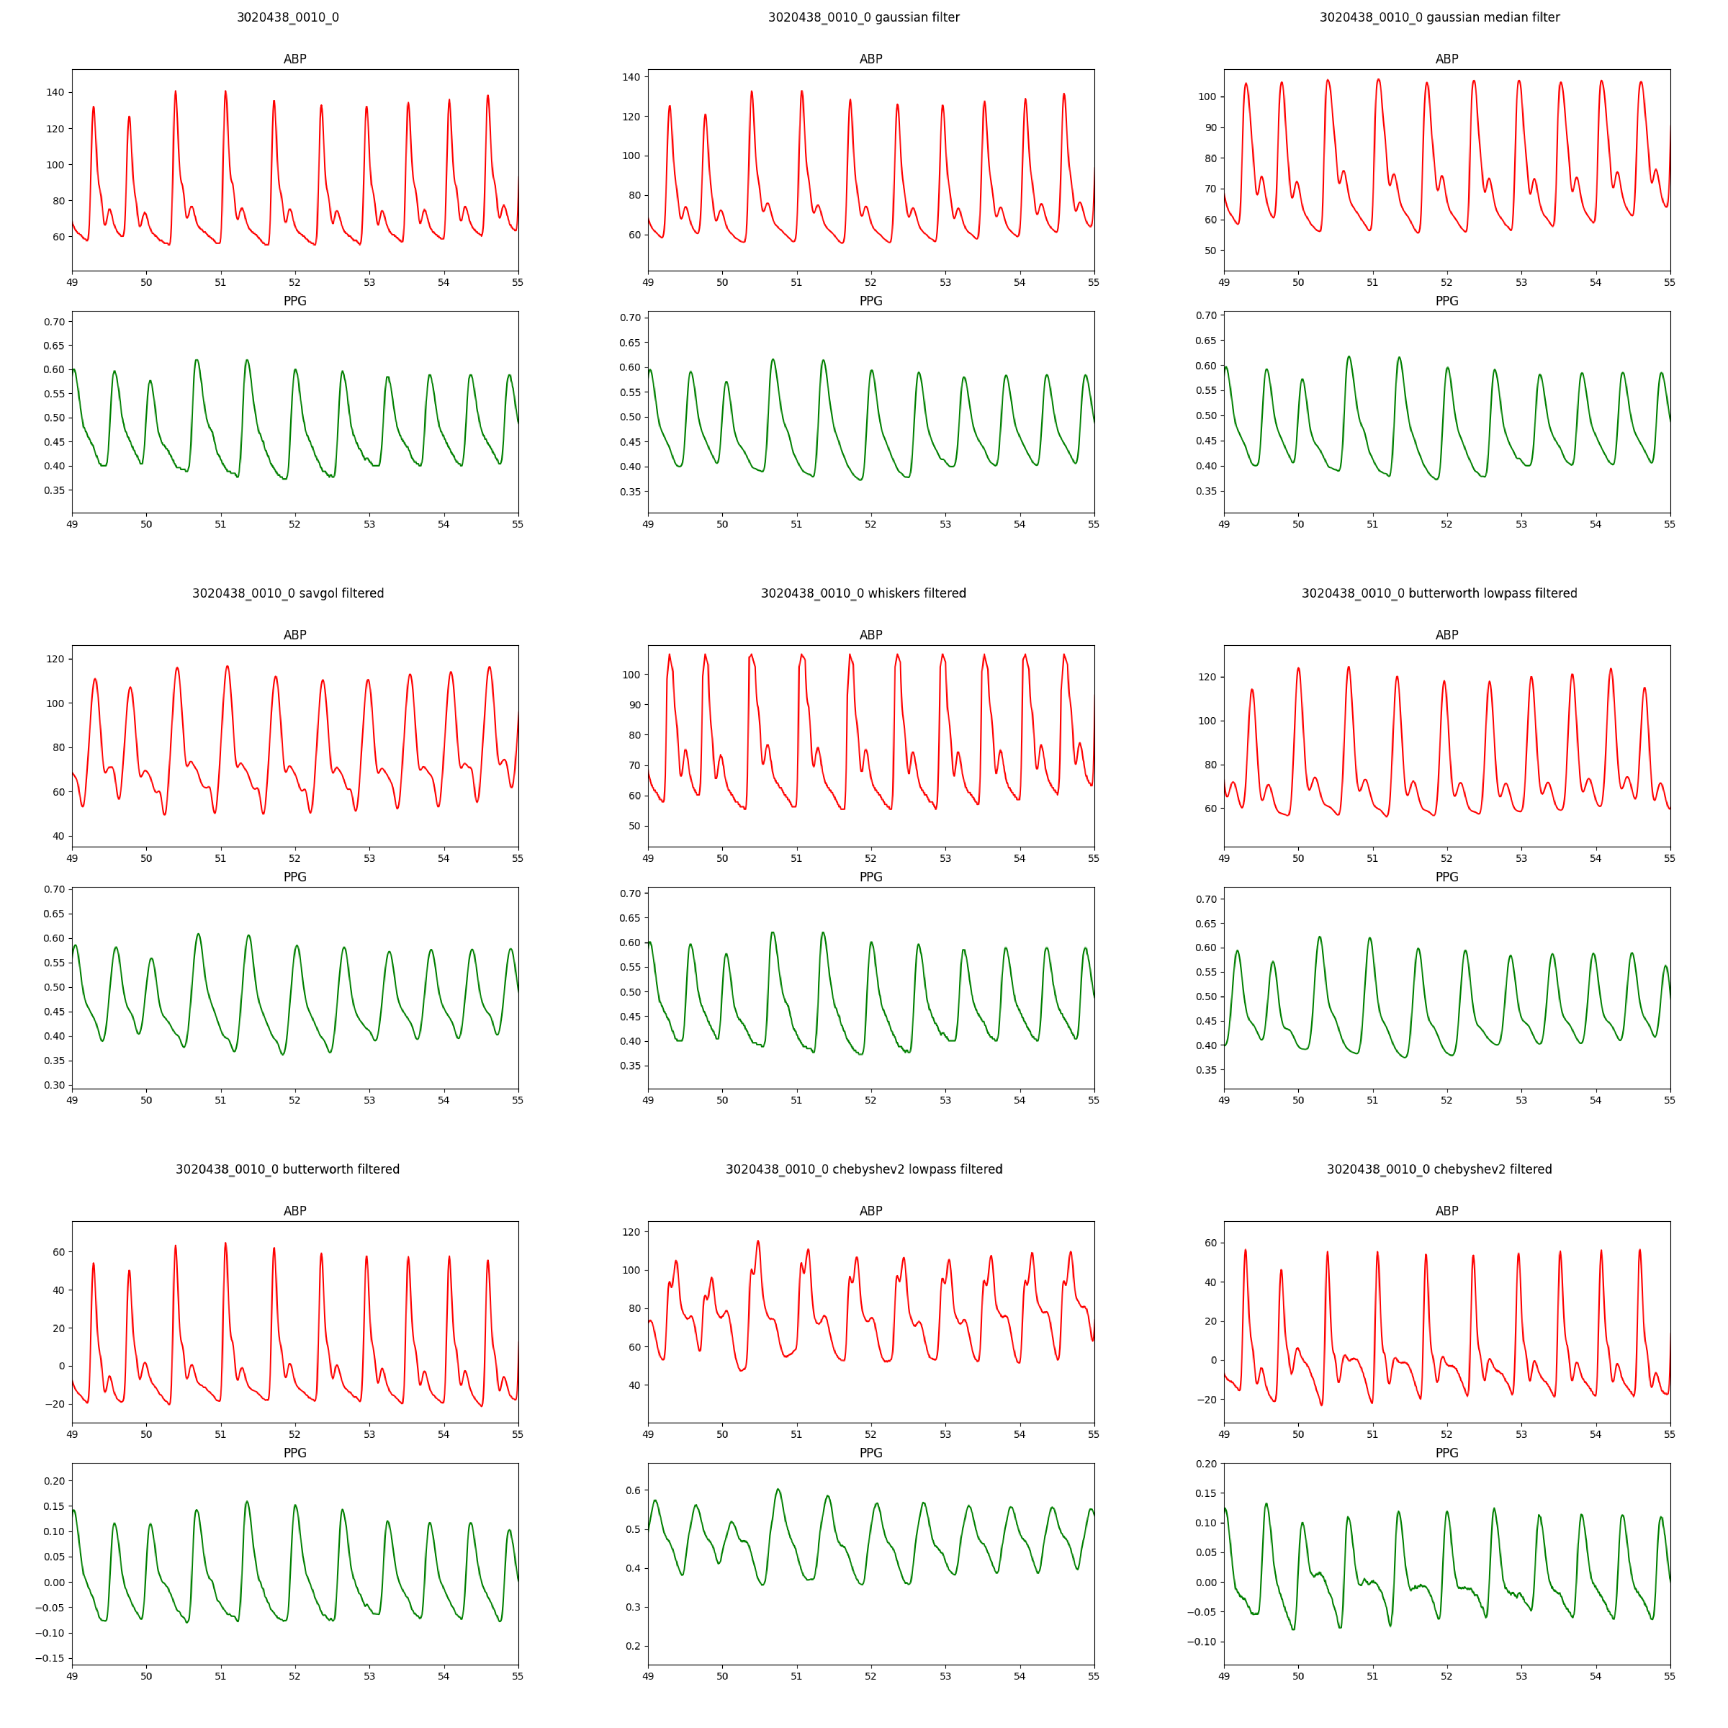
\includegraphics[width=0.9\textwidth]{images/methods/filters}
    \caption{9 different filters applied to the same ABP and PPG segment}
    \label{fig:filters}
\end{figure}

After a thorough evaluation of an extended set of filtered waveforms, the most effective strategy was determined:
The \textit{Savitzky-Golay} filter was selected to enhance the pulse wave shape, emphasizing the visualization of the dicrotic notch.
This was followed by the application of a \textit{Butterworth} lowpass filter to eliminate undesired frequencies and achieve noise reduction.
The impact of this filtering methodology is depicted in Figure~\ref{fig:opt_filtering}.

\begin{figure}[h]
    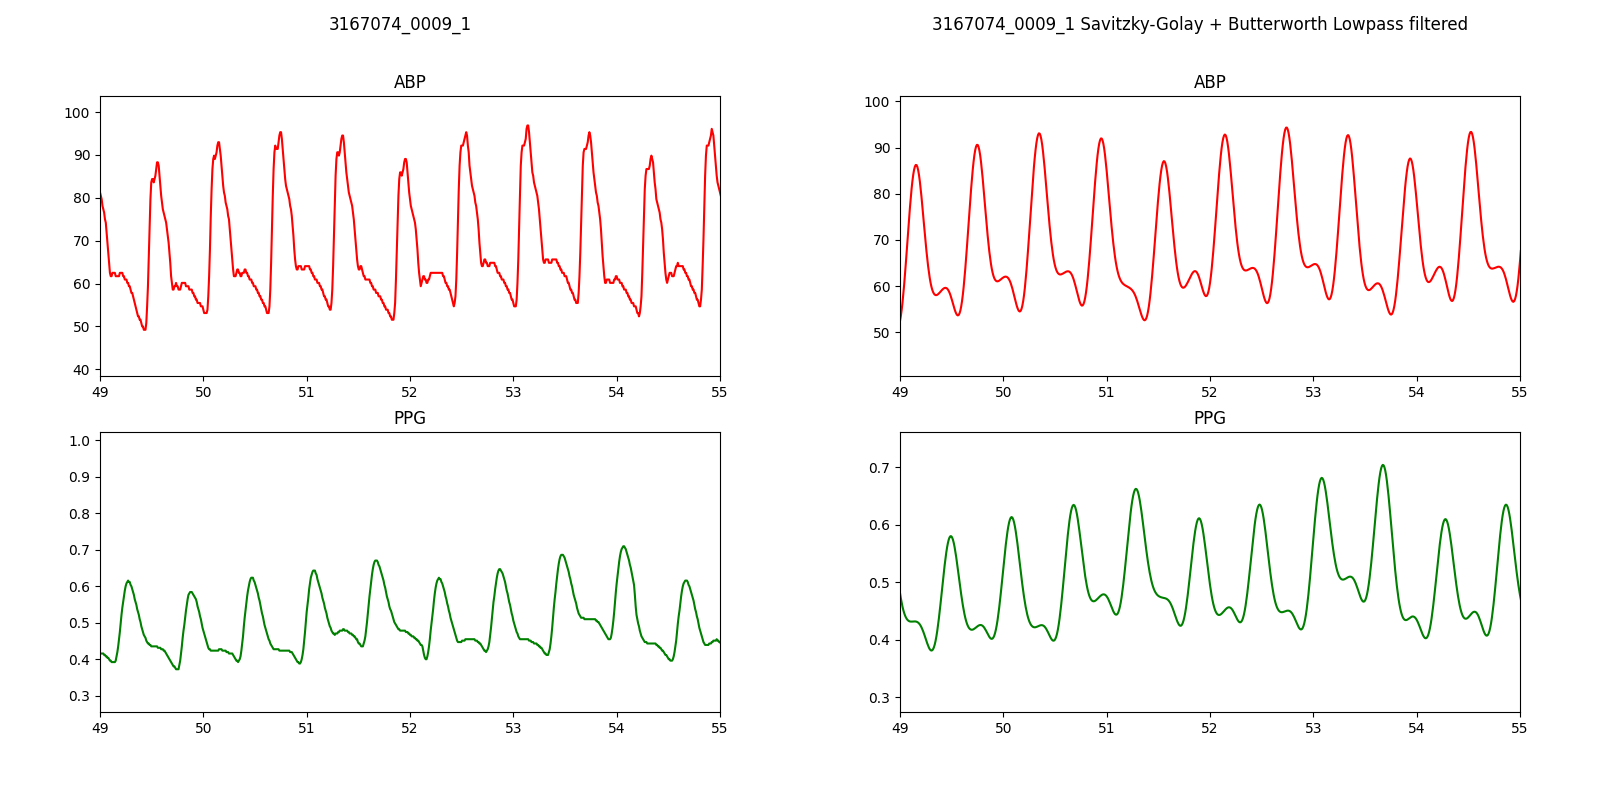
\includegraphics[width=0.9\textwidth]{images/methods/opt_filtering}
    \caption{Comparison of raw and optimally filtered PPG signals}
    \label{fig:opt_filtering}
\end{figure}

\subsubsection{Beat Finding Algorithms}
\label{subsubsec:beats}

The third stage of the signal processing phase involves Beat Detection, which is crucial for precisely identifying waveform peaks, facilitating the accurate extraction of fiducial points.
Moreover, precise beat detection enables the segmentation of the waveform into individual pulse waves, extending from pulse onset to offset, which is essential for subsequent PWA procedures.

The beat detection reference code was obtained from the openly available MIMIC WFDB Tutorial~\cite{charltonMIMICWFDBTutorials2022}.
Elisa Mejía-Mejía from City, University of London authored the \texttt{pulse\_detect()} method, which is publicly accessible in the \enquote{Tutorials/Beat detection/Functions} directory.
This method offers four distinct algorithms: \textit{HeartPy}~\cite{vangentHeartPyNovelHeart2019}, \textit{Second derivative maxima}~\cite{elgendiSystolicPeakDetection2013},
\textit{Systolic upslopes}~\cite{arguellopradaNovelLowcomplexityPeak2018} and \textit{Delineator}~\cite{aboyAutomaticBeatDetection2005}.
Each one of them is explained in more detail in the following paragraphs.

\vspace{0.2cm}
\textit{Beat Detection Algorithms}
\vspace{0.2cm}

For reference to the textual descriptions, the entire code of the following methods can be found in the appendix~\ref{subsec:code_beats}.

The \textit{HeartPy} beat detection algorithm identifies peaks in a pulsatile signal by comparing each data point to a moving average,
then determines inter-beat intervals based on the detected peaks, with the option for peak correction based on segment length.
The algorithm exhibited poor performance with the provided MIMIC datasets, detecting peaks inconsistently and occasionally crashing during operation,
consequently rendering it unsuitable for further integration.

The \textit{second derivative maxima} (also called the \textit{d2max}) algorithm applies a bandpass filter to the input pulsatile signal,
squares the filtered signal, and then identifies blocks of interest (BOIs) based on thresholding.
Within each BOI, it searches for peaks and selects the highest peak as the position of the inter-beat interval.

The shortest method \textit{upslopes} detects inter-beat intervals by analyzing upslopes in the input pulsatile signal.
It sets a threshold for identifying peaks based on the rate of upslope changes.
Peaks are detected when the upslope exceeds a certain threshold, and the position of each peak is recorded as the starting point of an inter-beat interval.

The last default algorithm, known as \textit{delineator}, processes waveforms by filtering the signal, computing thresholds based on peak and trough amplitudes,
and detecting peaks and onsets using predefined criteria.
It refines the detected peaks and onsets to improve accuracy and outputs the positions of the starting points of inter-beat intervals.

Precisely these last 3 methods were all implemented for beat finding.
Throughout the developmental stage, it became evident that these distinct methods exhibit considerable variability in beat detection, thereby preventing the selection of a singular method as the optimal choice.
A comparison algorithm was then initiated to assess these algorithms for every single waveform.

The performance comparison involved an automated analysis of the average number of detected pulses generated by each method, followed by the calculation of the difference between ABP and PPG pulses, with preference given to the method yielding the smaller discrepancy.
However, beyond mere discrepancy size, the overall size of the beat arrays also factored into the selection process.
Any method producing beat arrays significantly larger or smaller than the other two was regarded as an outlier and deemed unsuitable for the specific waveform.
Ultimately, the optimal beat array was determined based on the \enquote{difference percentage} measure, which is computed as the percentage ratio of the absolute difference between ABP and PPG pulses to the total pulses from both signals.
Thus, the optimal method was identified as the one generating larger beat arrays and exhibiting smaller differences between PPG and ABP\@.

One new method, termed \enquote{mean crossings}, was devised manually by the author.
This method involves computing the mean value of a signal, identifying crossings above and below this mean,
tallying their occurrences to determine a beat interval, and employing it as a variable for minimum distance to detect peaks in the signal.
\enquote{Mean crossings} was considered optimal only when its resultant beat arrays were larger in size and exhibited smaller inter-signal differences.

Examples for the results of each algorithm applied to different waveforms are illustrated in Figure~\ref{fig:beat_algos}, with black dots representing the detected pulse beats.

\begin{figure}[h]
    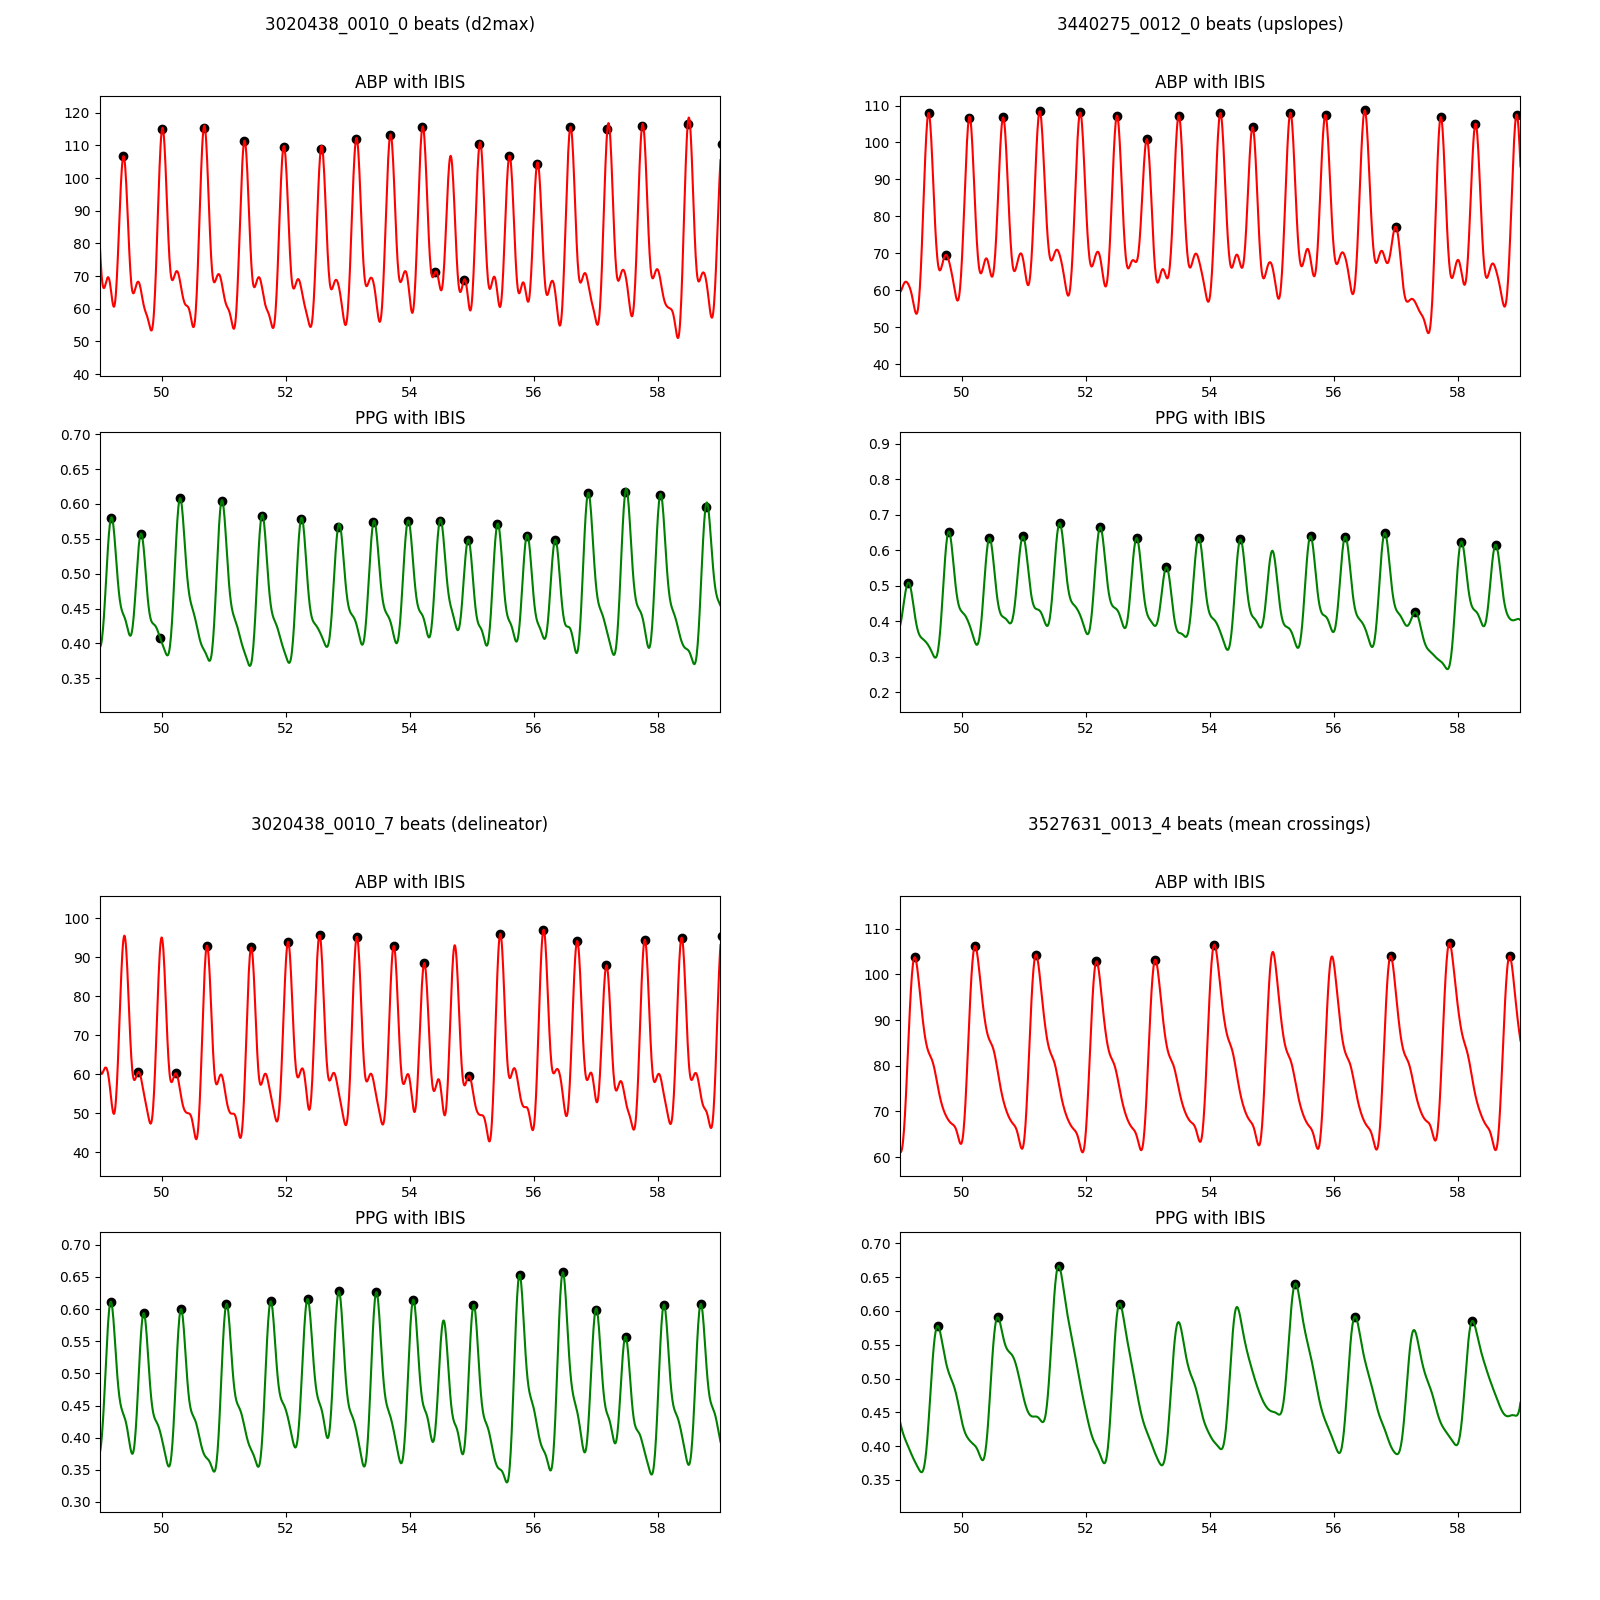
\includegraphics[width=0.9\textwidth]{images/methods/beat_algos}
    \caption{Application of 4 different beat finding algorithms}
    \label{fig:beat_algos}
\end{figure}

\vspace{0.2cm}
\textit{Selected Approach}
\vspace{0.2cm}

As already hinted in the description of the \enquote{mean crossings} algorithm, the optimal beat arrays were not utilized as the actual reference for beat timestamps, but solely for calculating the beat interval.
This was carried out to obtain a single variable, namely the \texttt{distance} parameter in a SciPy peak-finding function.
Experimentation revealed that this standard method was the most effective in identifying peaks in a waveform signal, and it was further refined using the \texttt{distance} and \texttt{prominence} parameters.
After trial and error, it was determined that three-quarters of the beat interval was the optimal \texttt{distance} value, while the \texttt{prominence} was set to 0.5 and 0.01 for ABP and PPG waveforms, respectively.
This methodology is illustrated in the following code snippet:

\vspace{0.1cm}
{\centering \texttt{abp\_beat\_interval = len(abp) / len(abp\_beats) \newline
ppg\_beat\_interval = len(ppg) / len(ppg\_beats) \newline
abp\_beats,\_=sp.find\_peaks(abp,distance=abp\_beat\_interval*.75,prominence=0.5) \newline
ppg\_beats,\_=sp.find\_peaks(ppg,distance=ppg\_beat\_interval*.75,prominence=0.01) \newline}}
\vspace{0.1cm}
\noindent and the improved accuracy of this approach is illustrated in Figure~\ref{fig:sp_beats}.

\begin{figure}[h]
    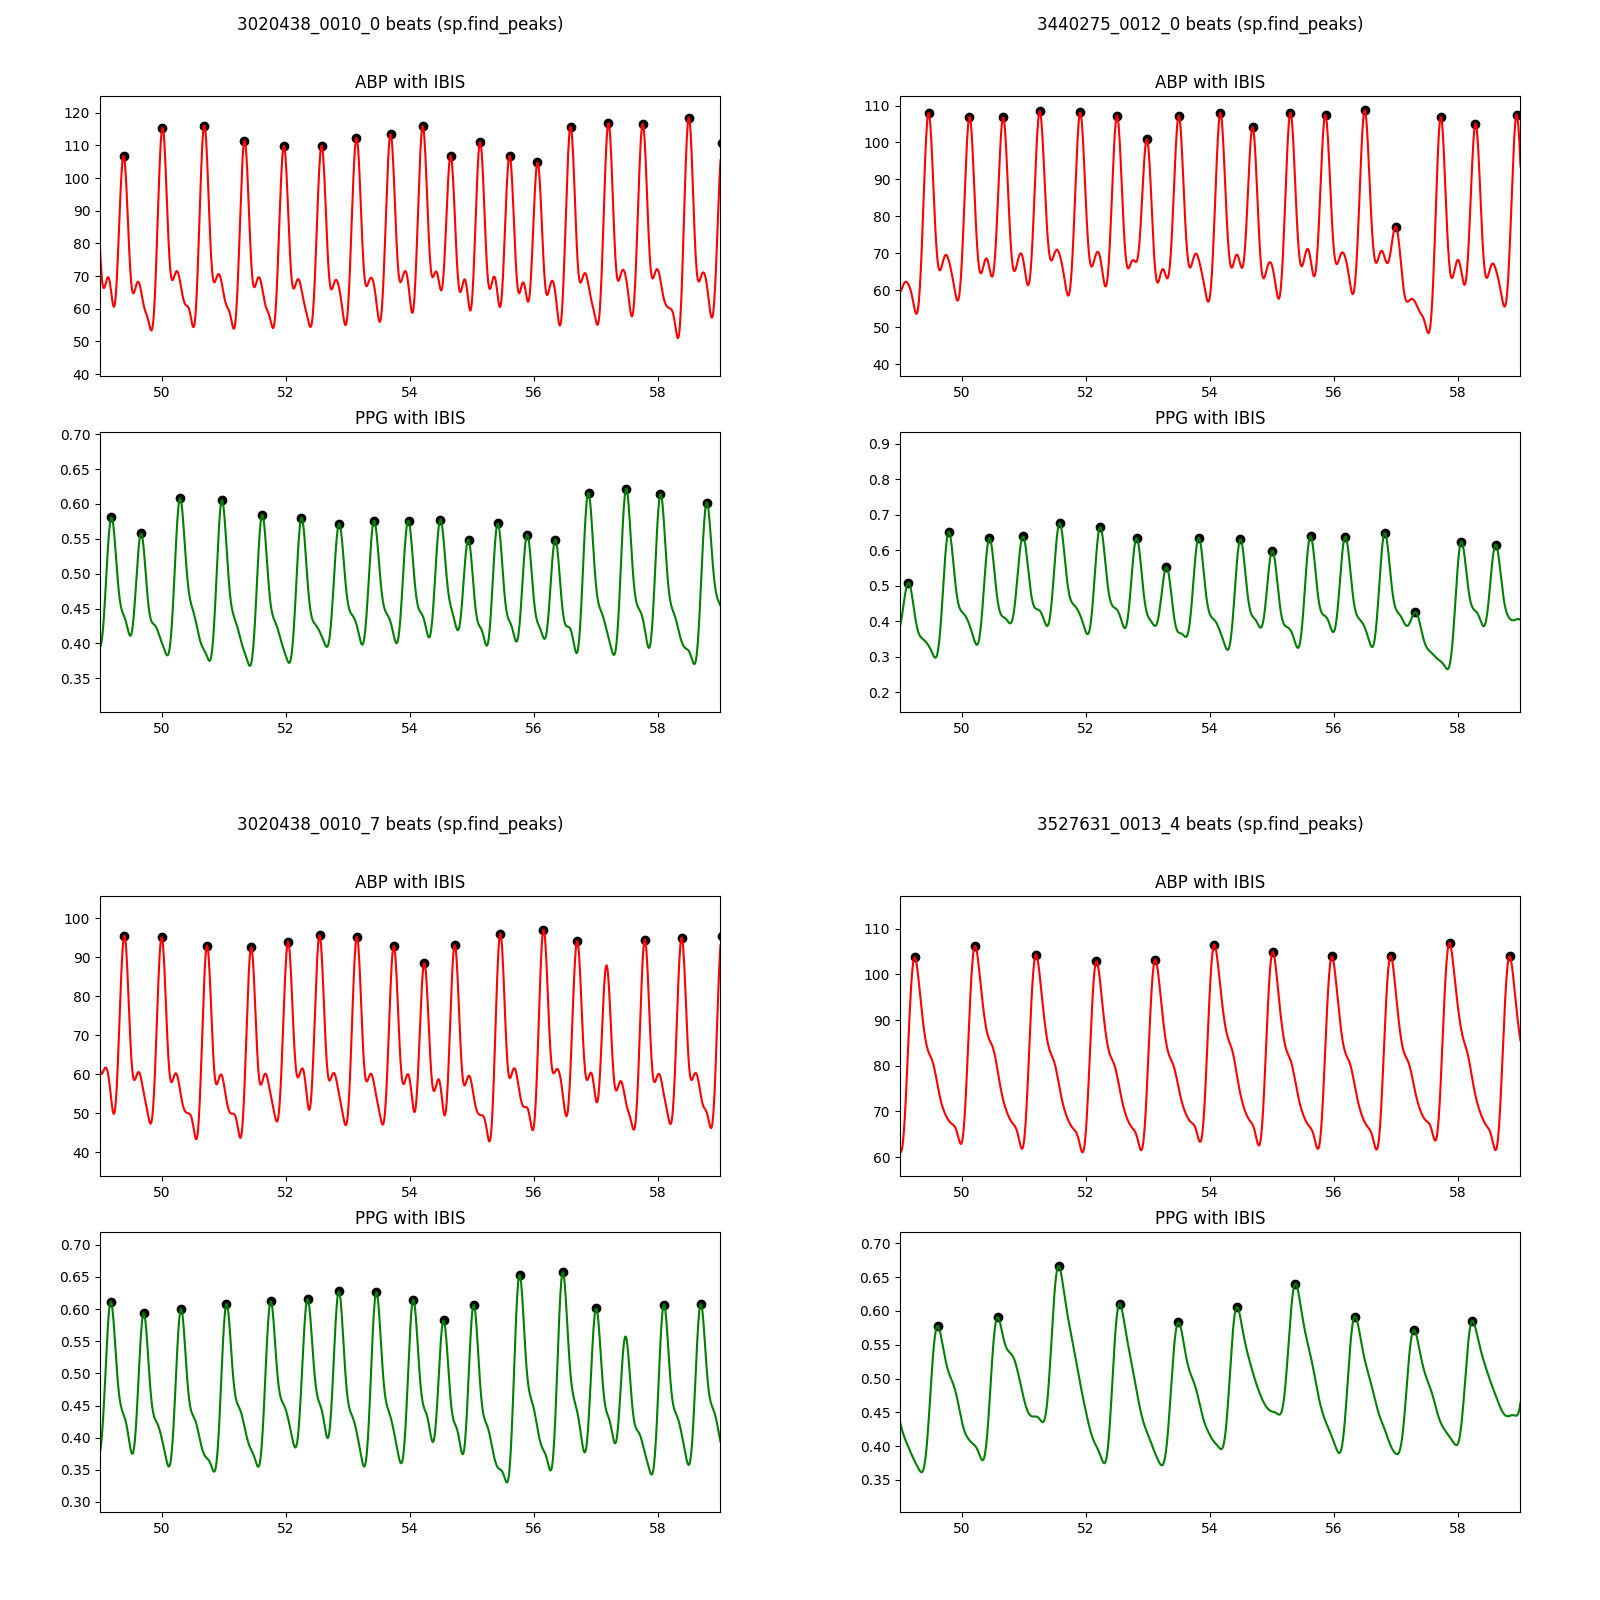
\includegraphics[width=0.9\textwidth]{images/methods/sp_beats}
    \caption{Application of the final beat finding approach on the same 4 waveforms as in Figure~\ref{fig:beat_algos}}
    \label{fig:sp_beats}
\end{figure}

In the rare event that this method also failed and fewer than 100 beats were found in the entire segment, the segment would be discarded, and the process would proceed to the next one.

\vspace{0.2cm}
\textit{Beat synchronization and grouping}
\vspace{0.2cm}

The final stage in generating an accurate beat timestamp array involves synchronization and grouping.

Due to a slight delay in the PPG waveform compared to the ABP signal (approximately 500 ms), synchronization becomes imperative.
This process entails identifying the closest PPG beat to the first ABP beat and vice versa, and the closest ABP beat to the last PPG beat.
Thereby splicing the respective arrays to produce two synchronized waveforms based on the indexes of the first and last PPG and ABP beats.

Additionally, it's crucial to address any instances of mis-detected beats in either signal.
For instance, if three ABP beats are detected at timestamps 50, 60, and 70, but only two beats are identified at timestamps 50 and 70 in the PPG waveform,
the ABP beat at timestamp 60 must be discarded as it lacks a corresponding PPG counterpart.
Consequently, the resulting beat arrays for both PPG and ABP waveforms possess identical lengths, with timestamps differing only marginally.

The effect of this final process is illustrated in Figure~\ref{fig:synchronized}.

\begin{figure}[h]
    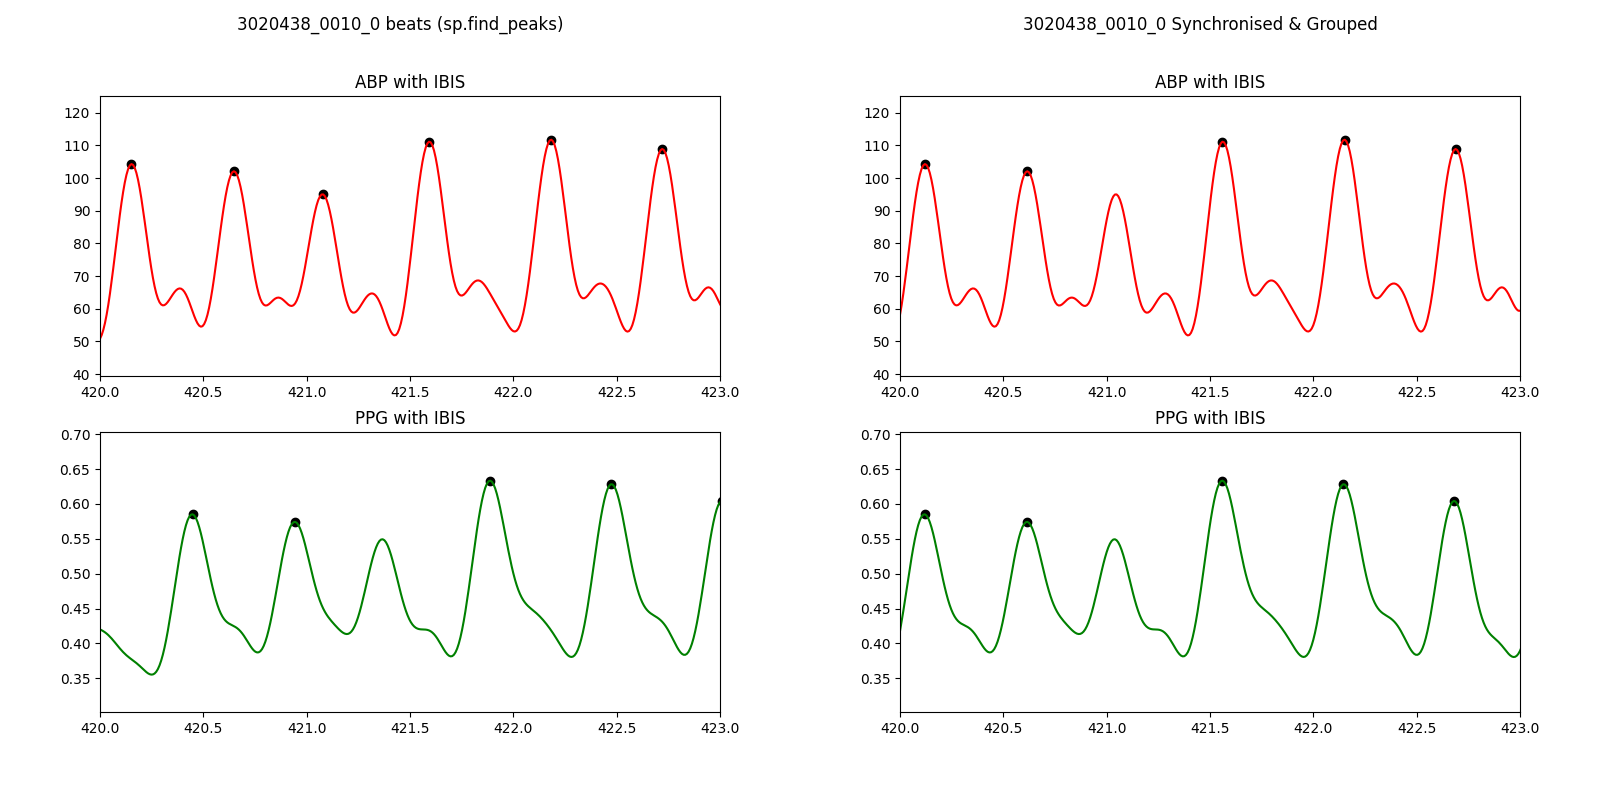
\includegraphics[width=0.9\textwidth]{images/methods/synchronised}
    \caption{Effect of beat synchronization and grouping}
    \label{fig:synchronized}
\end{figure}

\vspace{0.2cm}
\textit{Dealing with distorted signals}
\vspace{0.2cm}

An important aspect to highlight from the signal processing phase of the project is the management of irregular signals.
Two instances are depicted graphically in Figure~\ref{fig:distorted}.
The first plot exhibits a noticeable distortion in the PPG measurement, while the second plot likely portrays the waveform of a patient experiencing some form of arrhythmia.

\begin{figure}[h]
    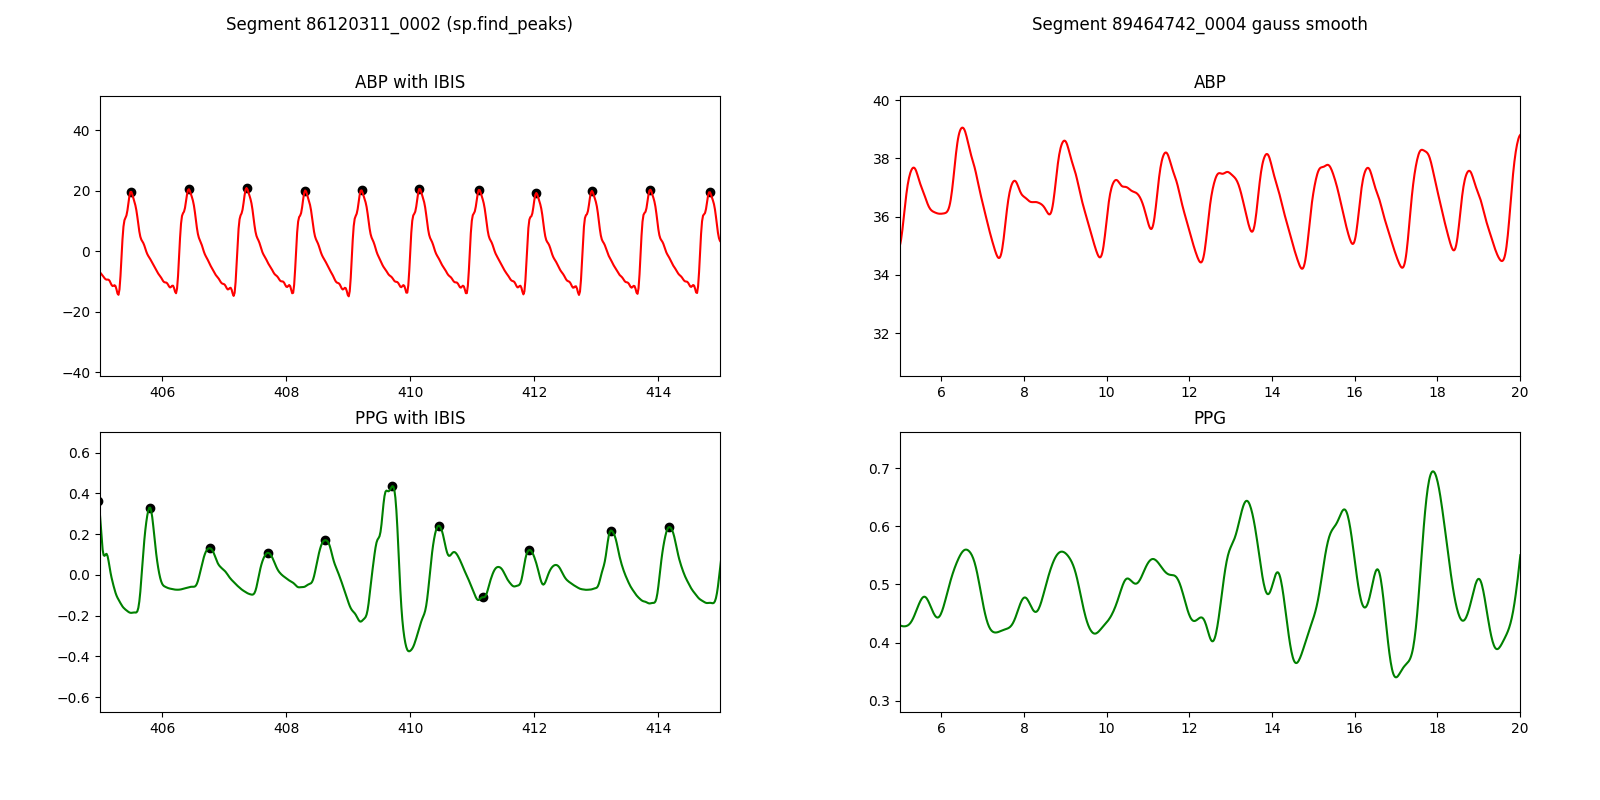
\includegraphics[width=0.9\textwidth]{images/methods/cringe_signals}
    \caption{Examples of distorted or irregular signals}
    \label{fig:distorted}
\end{figure}

In the scope of this project, manual selection of waveform shapes was not conducted, mainly due to the extensive size of samples.
Instead, the exclusion of irregular segments relied solely on programmed Exception Handling.
As previously discussed in the beat finding section, the rare occurrence of not finding 100 beats in a waveform may indicate a pathological heart function, as ensured by the following code:

\vspace{0.1cm}
{\texttt{\small if len(abp\_beats) < 100 or len(ppg\_beats) < 100: \newline
\indent\indent\indent raise Exception('Signal Processing failed: \newline
\indent\indent\indent\indent\indent\indent a substantial amount of beats not found')}}
\vspace{0.1cm}

Another issue occasionally encountered was the inconsistency in beat grouping.
This occurred when the beat finding algorithms generated arrays with significantly different beat timestamps, even post-synchronization.
If the beat grouping algorithm eliminated more than 5\% of the initial beats, it was considered a flawed array, leading to the exclusion of the current segment entirely.
This is exemplified by the following exception raised:

\vspace{0.1cm}
{\texttt{\small if (pre\_sync\_length) > (post\_sync\_length) * 1.05: \newline
\indent\indent\indent raise Exception('Signal Processing failed: \newline
\indent\indent\indent\indent\indent\indent too big of a difference after grouping')}}
\vspace{0.1cm}

\subsubsection{Fiducial Point Detection}
\label{subsubsec:fidp}

The fourth phase within the signal processing phase encompasses the detection of Fiducial Points (FIDPs), which is directly linked to feature extraction.

As detailed in the background section~\ref{subsec:computing_background}, this approach focuses on identifying distinct landmarks within a single pulse waveform.
Similarly to Pulse Detection, the framework for this segment was derived from the MIMIC WFDB Tutorial~\cite{charltonMIMICWFDBTutorials2022}, which is publicly accessible in the \enquote{Tutorials/Pulse Wave Analysis/Fiducial Point Functions} directory.
The \texttt{fiducial\_points()} function is designed to identify and adjust pulse-related signals by recognizing various FIDPs within cardiac cycles,
including systolic peaks, onsets, diastolic peaks, maximum slopes, and specific points derived from the second and third derivatives of the pulsatile signals.
Leveraging signal processing methodologies from NumPy, SciPy, and Matplotlib libraries, it determines the positions of these FIDPs based on the input pulsatile signal, peak positions, and sampling rate.
Moreover, it provides visualization capabilities to examine the detected points and their magnitudes, facilitating further analysis and enhancement of the FIDPs list.
The visualization of this function is provided in Figure~\ref{fig:wfdb_fidp}.

\begin{figure}[h]
    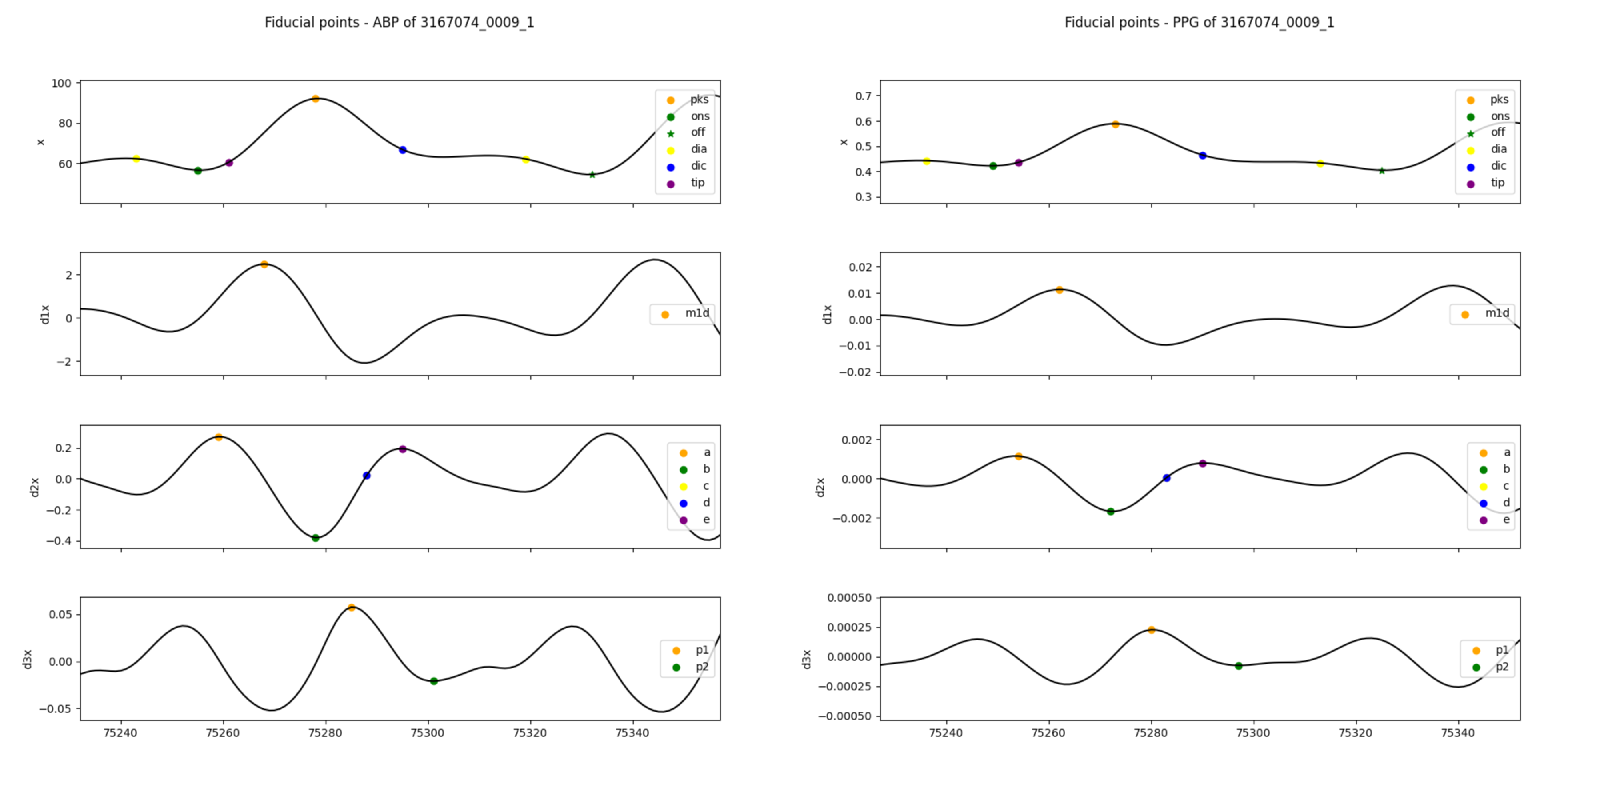
\includegraphics[width=0.9\textwidth]{images/methods/fidps}
    \caption{Example FIDP detection}
    \label{fig:wfdb_fidp}
\end{figure}

This method, akin to the pulse detection function, required refinement and enhancement to ensure smoother execution.
The details of these adjustments, along with the complete code, are available in the appendix~\ref{subsec:code_fidp}.

An important caveat to note pertains to the detection of the dicrotic notch.
As likewise discussed in the theoretical background section, the detectability of this fiducial point is greatly influenced by a patient's age and physical condition,
diminishing in clarity with advancing age and declining health.
Consequently, the extraction of fiducial points was constrained; not every waveform contained all the specified fiducial points (e.g., the dicrotic notch may have been absent).
Further insights into potential enhancements are provided in the discussion section~\ref{sec:discussion}.

\subsubsection{Feature Extraction}
\label{subsubsec:features}

The fifth and result-providing step of the signal processing phase is Feature Extraction.
It, as the name already hints at, is the most important part that provides the data for the creation and validation of ML models.
The methods of this section were created manually by selecting features on the basis of medical knowledge and past researches of this type~\cite{el-hajjDeepLearningModels2021, charltonAssessingHemodynamicsPhotoplethysmogram2022, maqsoodSurveyShallowDeep2022}.

\vspace{0.2cm}
\textit{PPG Features}
\vspace{0.2cm}

The following is a list of all extracted features from a single PPG pulse wave:
\begin{itemize}
    \item \texttt{sys}: the systolic peak amplitude value,
    \item \texttt{dia}: the diastolic dip, or lowest amplitude value after the systolic peak,
    \item \texttt{sys\_t}: systolic time - time difference between the systolic peak and the onset,
    \item \texttt{sys\_area}: systolic area - integral value of the signal over the time interval bounded by the onset and systolic peak,
    \item \texttt{dia\_t}: diastolic time - time difference between the offset and the systolic peak,
    \item \texttt{dia\_area}: diastolic area - integral value of the signal over the time interval bounded by the systolic peak and offset,
    \item \texttt{delta\_t}: delta time - time difference between the diastolic peak and the systolic peak,
    \item \texttt{delta\_area}: integral value of the signal over the time interval bounded by the systolic peak and the diastolic peak,
    \item \texttt{pulse\_area}: integral value of the signal over the time interval bounded by the onset and offset,
    \item \texttt{dia\_sys\_area\_ratio}: the ratio of diastolic area to the systolic area,
    \item \texttt{res\_index}: resistive index - ratio of difference between diastolic peak and offset values to difference between systolic peak and offset values,
    \item \texttt{vvi\_sys}: vessel volume fill-up (systolic) index - ratio of the systolic peak value to the maximum value among all systolic peaks,
    \item \texttt{vvi\_dia}: vessel volume drained (diastolic) index - ratio of the minimum value among all offset values to the offset value,
    \item \texttt{dw10}: diastolic width at 10\% amplitude - time duration between systolic peak and offset at 10\% pulse amplitude,
    \item \texttt{dw+sw10}: sum of diastolic and systolic widths at 10\% amplitude (systolic width is time duration between onset at 10\% amplitude and systolic peak),
    \item \texttt{dw/sw10}: ratio of diastolic width to systolic width both at 10\% amplitude,
    \begin{multicols}{6}
        \item \texttt{dw25} \columnbreak
        \item \texttt{dw+sw25} \columnbreak
        \item \texttt{dw/sw25} \columnbreak
        \item \texttt{dw33} \columnbreak
        \item \texttt{dw+sw33} \columnbreak
        \item \texttt{dw/sw33} \columnbreak
    \end{multicols}
    \begin{multicols}{6}
        \item \texttt{dw50} \columnbreak
        \item \texttt{dw+sw50} \columnbreak
        \item \texttt{dw/sw50} \columnbreak
        \item \texttt{dw75} \columnbreak
        \item \texttt{dw+sw75} \columnbreak
        \item \texttt{dw/sw75} \columnbreak
    \end{multicols}
    \item \texttt{mean\_frequency}: weighted average of positive frequencies in the magnitude spectrum obtained through the FFT,
    \item \texttt{total\_power}: sum of magnitudes of all frequency components in the FFT result, indicating the overall energy of the signal in the frequency domain,
    \item \texttt{normalized\_power\_at\_peak}: relative contribution of the peak frequency component to the total power of the signal computed through the FFT\@.
\end{itemize}

All features apart from the last 3 are extracted from the direct PPG pulse wave by calculating the values either from timestamps of the PPG amplitude values - all of them are regarded as time domain features.
The last three features are regarded as frequency domain features, since the values are calculated from the FFT, which is represented in the following function:

\begin{center}
    \begin{math}
        X(k) = \sum_{n=0}^{N-1} x(n) e^{-i 2\pi kn/N}
    \end{math}
\end{center}

\begin{flushleft}
    \small
    \begin{tabular}{ll}
        $X(k)$ & : Discrete Fourier Transform (DFT) coefficients at frequency index $k$ \\
        $x(n)$ & : Input signal data point at time index $n$                            \\
        $N$    & : Total number of samples in the input signal                          \\
        $k$    & : Frequency index ranging from $0$ to $N-1$                            \\
    \end{tabular}
\end{flushleft}

The code for the extraction of each feature can be found in the appendix~\ref{subsec:code_fe}.
The visualization of time and frequency domain features can be found in Figure~\ref{fig:td_feats} and~\ref{fig:fd_feats} respectively.

\begin{figure}[h]
    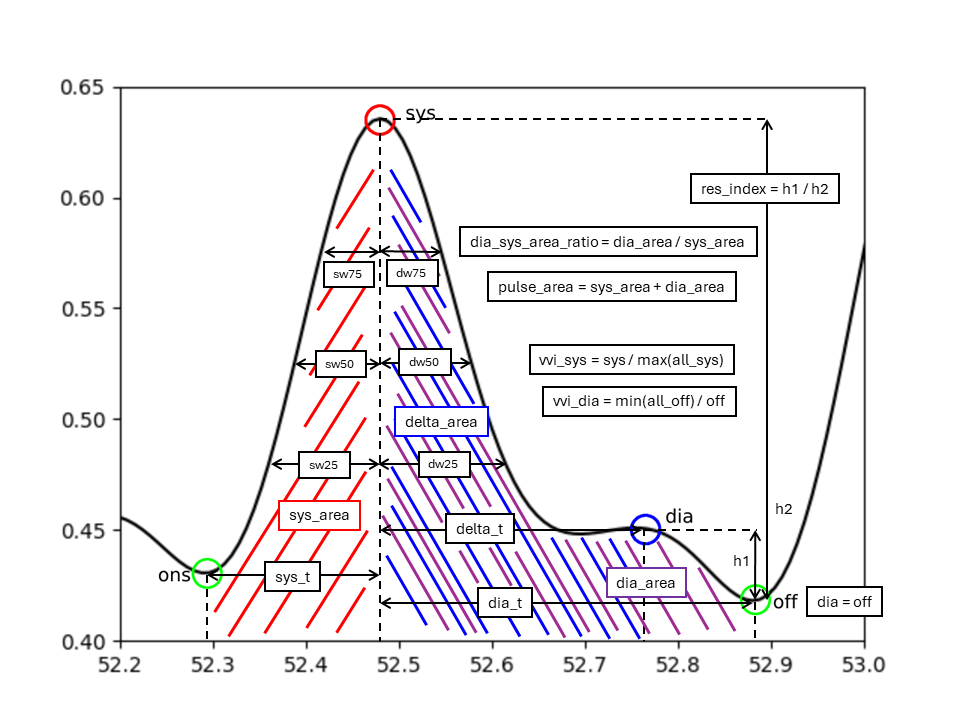
\includegraphics[width=0.9\textwidth]{images/methods/feats}
    \caption{Time domain features}
    \label{fig:td_feats}
\end{figure}

\begin{figure}[h]
    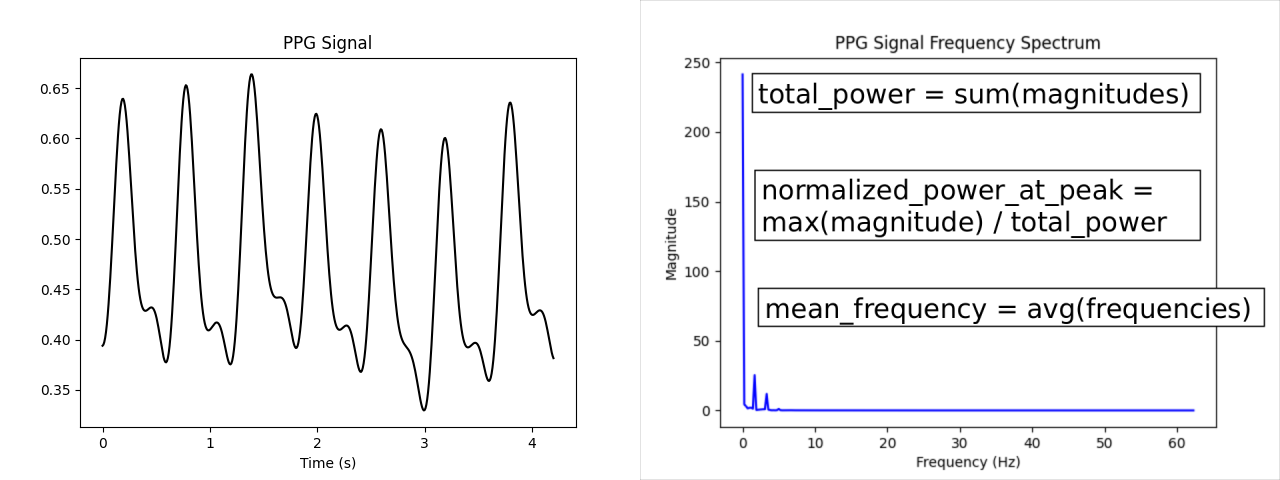
\includegraphics[width=0.9\textwidth]{images/methods/median_fft}
    \caption{Frequency domain features}
    \label{fig:fd_feats}
\end{figure}

\vspace{0.2cm}
\textit{ABP Features}
\vspace{0.2cm}

Three specific features were selected for extraction from the ABP waveform to serve as the target prediction values.
These features encompassed the Systolic Pressure (SP), Diastolic Pressure (DP), and Mean Arterial Pressure (MAP).
The determination of the SP and DP involved a straightforward method of extracting the values of the \texttt{sys} and \texttt{off} FIDPs (see Figure~\ref{fig:wfdb_fidp}).
Lastly, the calculation method employed for the MAP values was based on the formula provided by DeMers and Wachs~\cite{demersPhysiologyMeanArterial2024}:

\vspace{0.1cm}
\large
\begin{center}
    \begin{math}
        \texttt{MAP} = \texttt{DP} + \left(\frac{\texttt{SP} - \texttt{DP}}{3}\right).
    \end{math}
\end{center}
\normalsize

\vspace{0.2cm}
\textit{Total and median values}
\vspace{0.2cm}

The last step taken in the feature extraction, was the median value extraction over a specific beat window.
Measuring the median values over a specific PPG window offers several advantages over simply taking the absolute values from every single pulse wave.
Firstly, calculating the median helps to mitigate the influence of outliers or irregularities in individual pulse waves, providing a more robust representation of the underlying physiological state.
By capturing the central tendency of the data within each window, the median value offers a more stable and reliable estimate of the overall signal characteristics.
Additionally, median values effectively filter out any left-over noise from the pre-processing part, making them more reliable measures compared to absolute values.
Finally, this approach reduces the computational complexity compared to dealing with total features extracted from each pulse wave individually, making it more efficient for large-scale data processing tasks, such as ML model training.
Specifically these median values were the ones used in all subsequent ML processes.

Through empirical investigation, it was determined that a window of 7 consecutive beats served as the most effective median interval
for computing feature values from both PPG and ABP signals.
Within this interval, the median values for all features were computed, with the exception of frequency domain features.
For the frequency domain features, the FFT was applied to the entire 7-beat window, extracting values from the complete segment as illustrated in Figure~\ref{fig:fd_feats}.

\subsection{Machine Learning}
\label{subsec:ml_methods}

In this concluding section detailing methods, the utilization of Machine Learning methodologies is elaborated upon,
drawing from a range of studies as referenced in the background section~\ref{subsubsec:machine_learning}.
This study employed diverse models, distinct strategies for data splitting, and methods for training and validation.

The use of \textit{Scikit-Learn}~\cite{ScikitlearnMachineLearning} (version 1.4) was employed for simpler regression models within this study.
Utilizing version 2.2 of \textit{PyTorch}~\cite{PyTorch}, the library was enhanced with the CUDA toolkit for GPU acceleration in the context of NN processes.
The library \textit{wandb}~\cite{Wandb} was employed for the purpose of monitoring and visualizing the model's performance.

Initially, the PPG and ABP data were delineated as \texttt{X} and \texttt{y} correspondingly.
Then, data from the MIMIC-III DB was partitioned randomly adhering to the 80/20 training/testing proportions.
Following this, all data underwent normalization utilizing the \texttt{sklearn.preprocessing.StandardScaler} class.
This step was implemented to accommodate variations in feature scales and to guarantee an equal contribution of each feature to the analysis.

After this initial phase, the training of the models commenced.
A total of 8 regression models were implemented:
\begin{itemize}
    \item Linear Regression (\textit{PyTorch}),
    \item Multi-Layer Perceptron (\textit{PyTorch}),
    \item Long Short-term memory model (\textit{PyTorch}),
    \item bi-directional LSTM (\textit{PyTorch}),
    \item Gated Recurrent Unit (\textit{PyTorch}),
    \item bi-directional GRU (\textit{PyTorch}),
    \item Random Forest Regressor (\textit{Scikit-Lear})
    \item Support Vector Regressor (\textit{Scikit-Learn})
\end{itemize}

The code of the listed ML models can be found in appendix~\ref{subsec:code_ml}.

In LR and MLP models, the utilized optimizers were \enquote{Stochastic Gradient Descent} (SGD)\cite{SGDPyTorchDocumentation} and \enquote{Adaptive Moment Estimation} (Adam)\cite{AdamPyTorchDocumentationa} respectively.
The optimizer for LSTM and GRU models was \enquote{Limited-memory Broyden–Fletcher–Goldfarb–Shanno} (LBFGS) algorithm~\cite{LBFGSPyTorchDocumentation}, each running for 100 epochs with a learning rate set to 0.1.

The SVR model was initialized with the \texttt{linear} kernel, a regularization parameter \texttt{C} set to 100, and with an \texttt{epsilon} of 0.1.
The \enquote{RandomForestRegressor} model was configured with 100 decision trees, each restricted to a maximum depth of 10 nodes, and a minimum of 2 samples required to split an internal node.

During the training phase, the \enquote{Mean-Squared-Error} (MSE) loss was computed and used as the performance reference.
MSE is generally favoured in continuous value regression endeavors, because it gives more weight to larger errors, especially outliers.
For \textit{PyTorch} models, an \enquote{early-stopping} strategy was implemented, halting training if the testing loss did not improve for 3 consecutive epochs.

After the training step, an evaluation of feature importance was conducted, employing a method that assesses each feature's significance by permuting their values and observing the resulting impact on model performance.
This was followed by a subsequent identical iteration of the model, differing only by the incorporation of added weights to the most crucial features.

For the testing evaluation in both iterations, the chosen metrics included \textit{Root Mean-Squared-Error} (RMSE), \textit{Mean Absolute Error} (MAE), \textit{$R^2$} measure, \textit{Bias}, and \textit{Limits-of-Agreement} (LoA).

Finally, the dataset from the MIMIC-IV DB was utilized for model validation.
The same data normalization techniques were applied as in the training stage.
Following the prediction of ABP, the resulting dataset was split into three, encompassing the predicted values of SP, DP, and MAP\@.
RMSE and MAE values were calculated for the entire prediction dataset, as well as for each of the three separate predicted value arrays.
Precisely these metrics effectively portrayed the ultimate accuracy of the model in predicting ABP (SP, DP and MAP).



    \section{Results}
    \label{sec:results}
    \subsection{Data Fetching}
\label{subsec:data_fetching}

Data for Validation from MIMIC4:
5508 records each containing 37795 values corresponding to ~605 seconds (fs=64.4725);

Data for Training/Testing from MIMIC3:
22083 (~4*MIMIC4) records each containing 75625 values corresponding to 605 seconds (fs=125);

\subsection{Feature Extraction}
\label{subsec:feature_extraction}

\begin{table}{\textwidth}
    \renewcommand{\arraystretch}{1.5}
    \setlength{\tabcolsep}{12pt}
    \begin{center}
        \begin{tabular}{ |c|c|c| }
            \hline
            & MIMIC-III  & MIMIC-IV  \\
            \hline
            Records       & 22,083     & 5,508     \\
            \hline
            Total Values  & 13,659,375 & 1,309,265 \\
            \hline
            Median Values & 1,918,623  & 183,140   \\
            \hline
        \end{tabular}
    \end{center}
    \captionsetup{format=plain, justification=centering}
    \caption{Fetched and Extracted Data from MIMIC-III and MIMIC-IV DBs}
    \label{tab:records}
\end{table}

FE from MIMIC4 for Validation:
- For target reference Systolic, Diastolic and MAP values were extracted from the waveform data.
- For Machine Learning, 34 features were extracted from the PPG waveform
A total of \textbf{1,309,265} values were extracted, resulting in a 34 x 1,309,265 matrix.
Total of \textbf{183,140} median values were extracted.

FE from MIMIC3 for Training/Testing:

- For target reference ABP Systolic, Diastolic and MAP values were extracted from the waveform data.
- For Machine Learning, 34 features were extracted from the PPG waveform
A total of \textbf{13,659,375} values were extracted, resulting in a 34 x 13659375 matrix.
Total of \textbf{1,918,623} median values were extracted.

The summarized results are displayed in Table~\ref{tab:records}.
Data Flow is visualized in Figure~\ref{fig:data_flow}.

\begin{figure}[h]
    \centering
    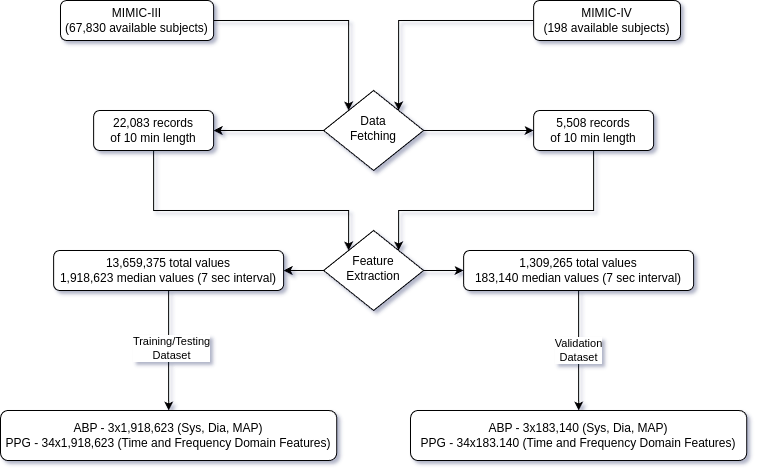
\includegraphics[width=0.9\textwidth]{images/results/flow_diagram}
    \caption{Flow Diagram presenting the Data Fetching and Processing}
    \label{fig:data_flow}
\end{figure}

\subsection{Machine Learning}
\label{subsec:machine_learning}

\begin{center}
    \begin{tabular}{ |c|c|c|c| }
        \hline
        & Training Loss (MSE) & Testing Loss (MSE) & Testing MAE \\
        \hline
        LR                     & 218.443             & -                  & 11.097      \\
        \hline
        MLP                    & 208.343             & -                  & 10.866      \\
        \hline
        LSTM                   & 93.81               & 97.358             & 6.953       \\
        \hline
        LSTM (weight adjusted) & 97.615              & 100.498            & 7.085       \\
        \hline
        Bi-LSTM                & -                   & -                  & -           \\
        \hline
        GRU                    & 88.34               & 92.142             & 6.759       \\
        \hline
        GRU (weight adjusted)  & 88.167              & 90.955             & 6.727       \\
        \hline
        Bi-GRU                 & -                   & -                  & -           \\
        \hline
        SVR                    & -                   & -                  & -           \\
        \hline
        RF                     & -                   & -                  & -           \\
        \hline
    \end{tabular}
\end{center}

\begin{center}
    \begin{tabular}{ |c|c|c|c| }
        \hline
        & Testing RMSE & Validation RMSE & Validation MAE \\
        \hline
        LR                     & 14.777       &                 &                \\
        \hline
        MLP                    & 14.446       &                 &                \\
        \hline
        LSTM                   & 9.866        & -               & 14.597         \\
        \hline
        LSTM (weight adjusted) & 10.024       & -               & 14.646         \\
        \hline
        Bi-LSTM                & -            & -               & -              \\
        \hline
        GRU                    & 9.598        & -               & 14.951         \\
        \hline
        GRU (weight adjusted)  & 9.536        & -               & 15.205         \\
        \hline
        Bi-GRU                 & -            & -               & -              \\
        \hline
        SVR                    & -            & -               & -              \\
        \hline
        RF                     & -            & -               & -              \\
        \hline
    \end{tabular}
\end{center}

LSTM \& GRU training and testing loss charts (32 \& 33) % (\ref{fig:train_mse} \& \ref{fig:test_mse}).

Feature Importance chart in Figure~34 (at the end of the document) % \ref{fig:feat_importance} (at end of document).

%\begin{figure}
%    \centering
%    \begin{subfigure}{0.5\textwidth}
%        \centering
%        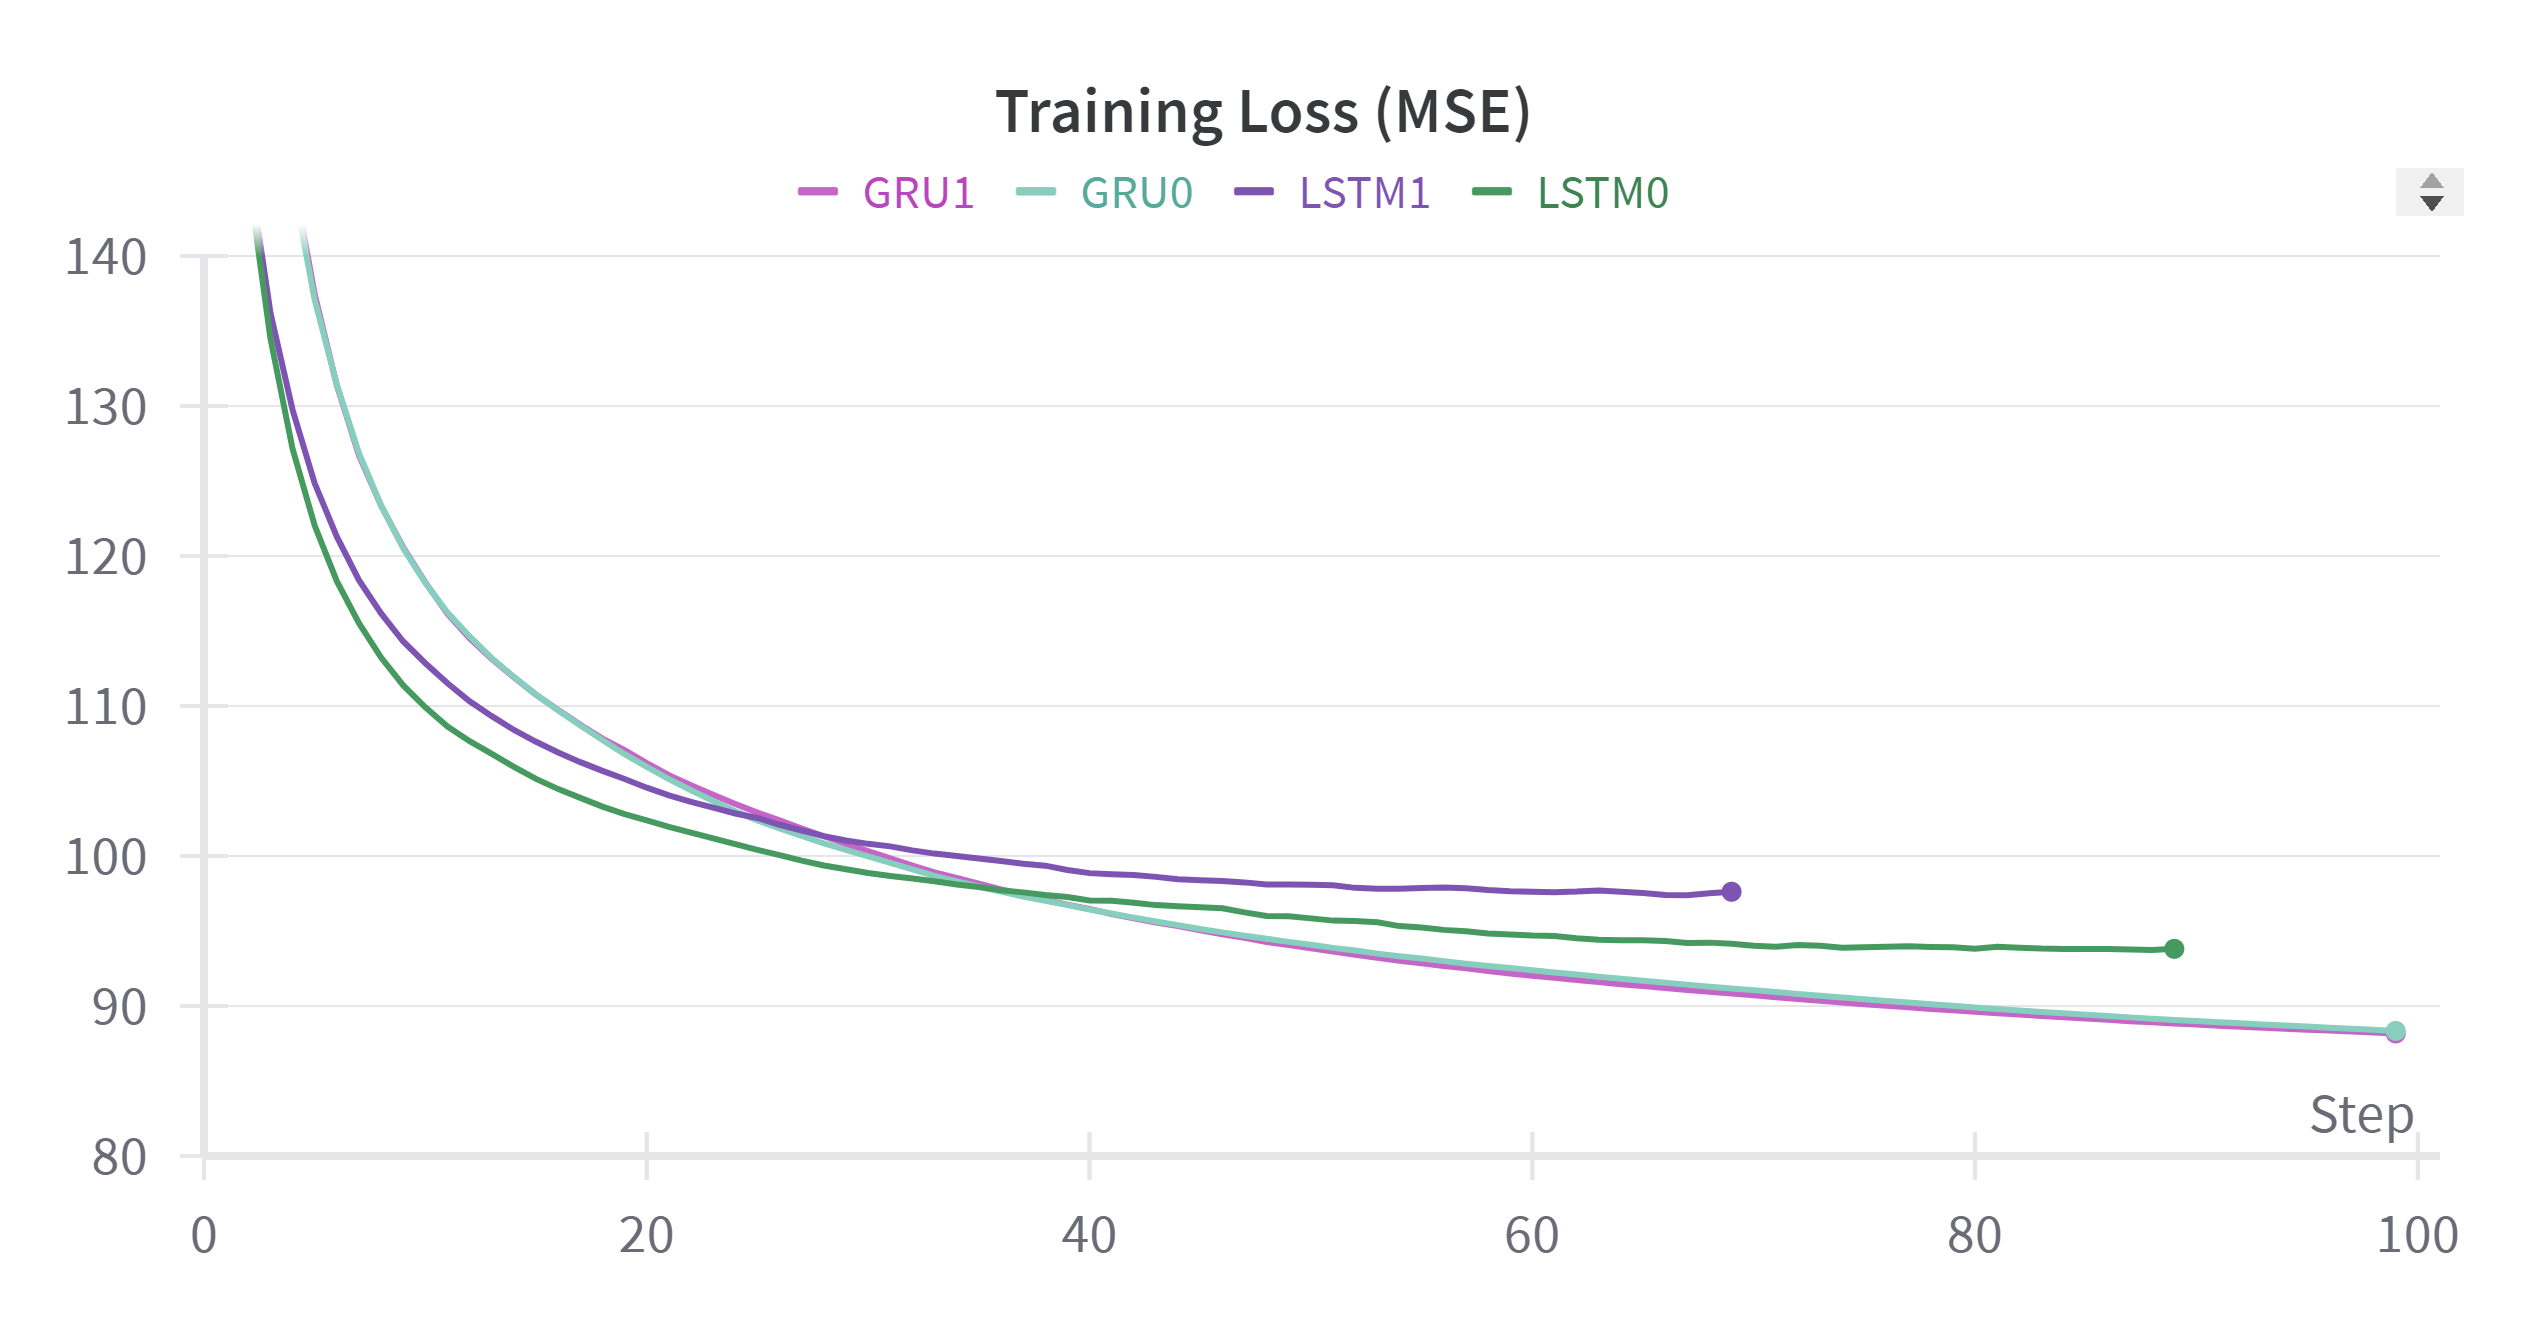
\includegraphics[width=0.4\linewidth]{images/results/LSTM_GRU_Train_mse}
%        \caption{LSTM \& GRU Train MSE}
%        \label{fig:train_mse}
%    \end{subfigure}
%    \begin{subfigure}{0.5\textwidth}
%        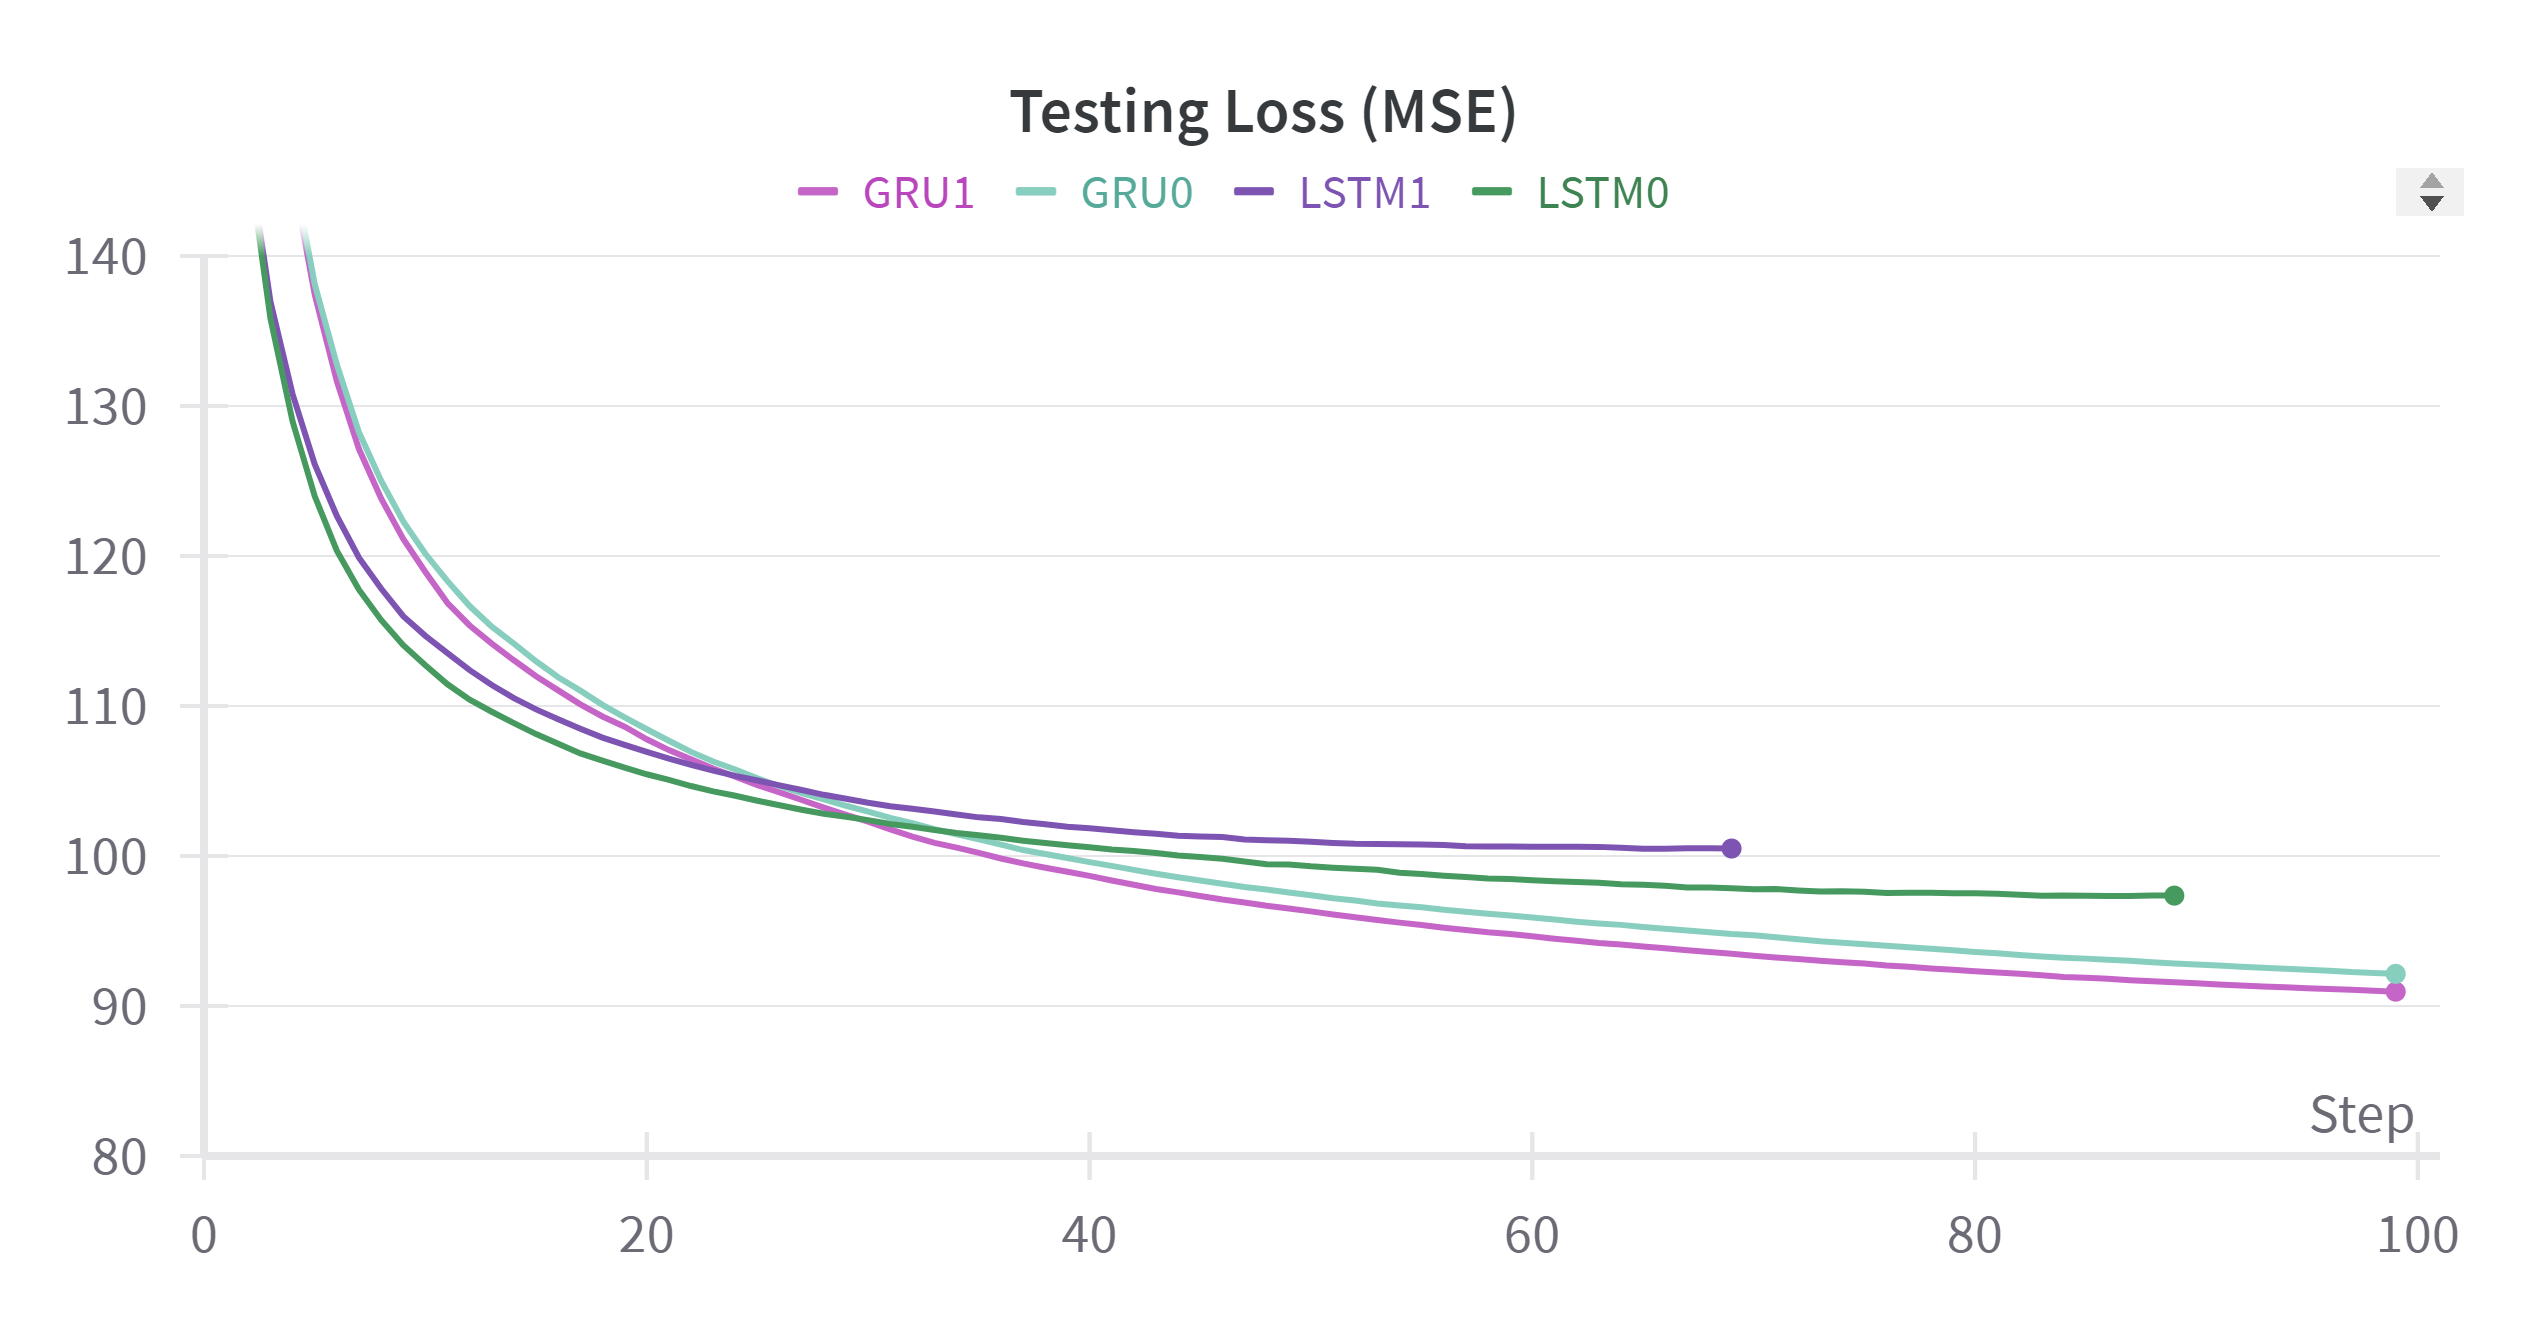
\includegraphics[width=0.4\linewidth]{images/results/LSTM_GRU_Test_mse}
%        \caption{LSTM \& GRU Test MSE}
%        \label{fig:test_mse}
%    \end{subfigure}
%\end{figure}

\begin{figure}[h]
    \centering
    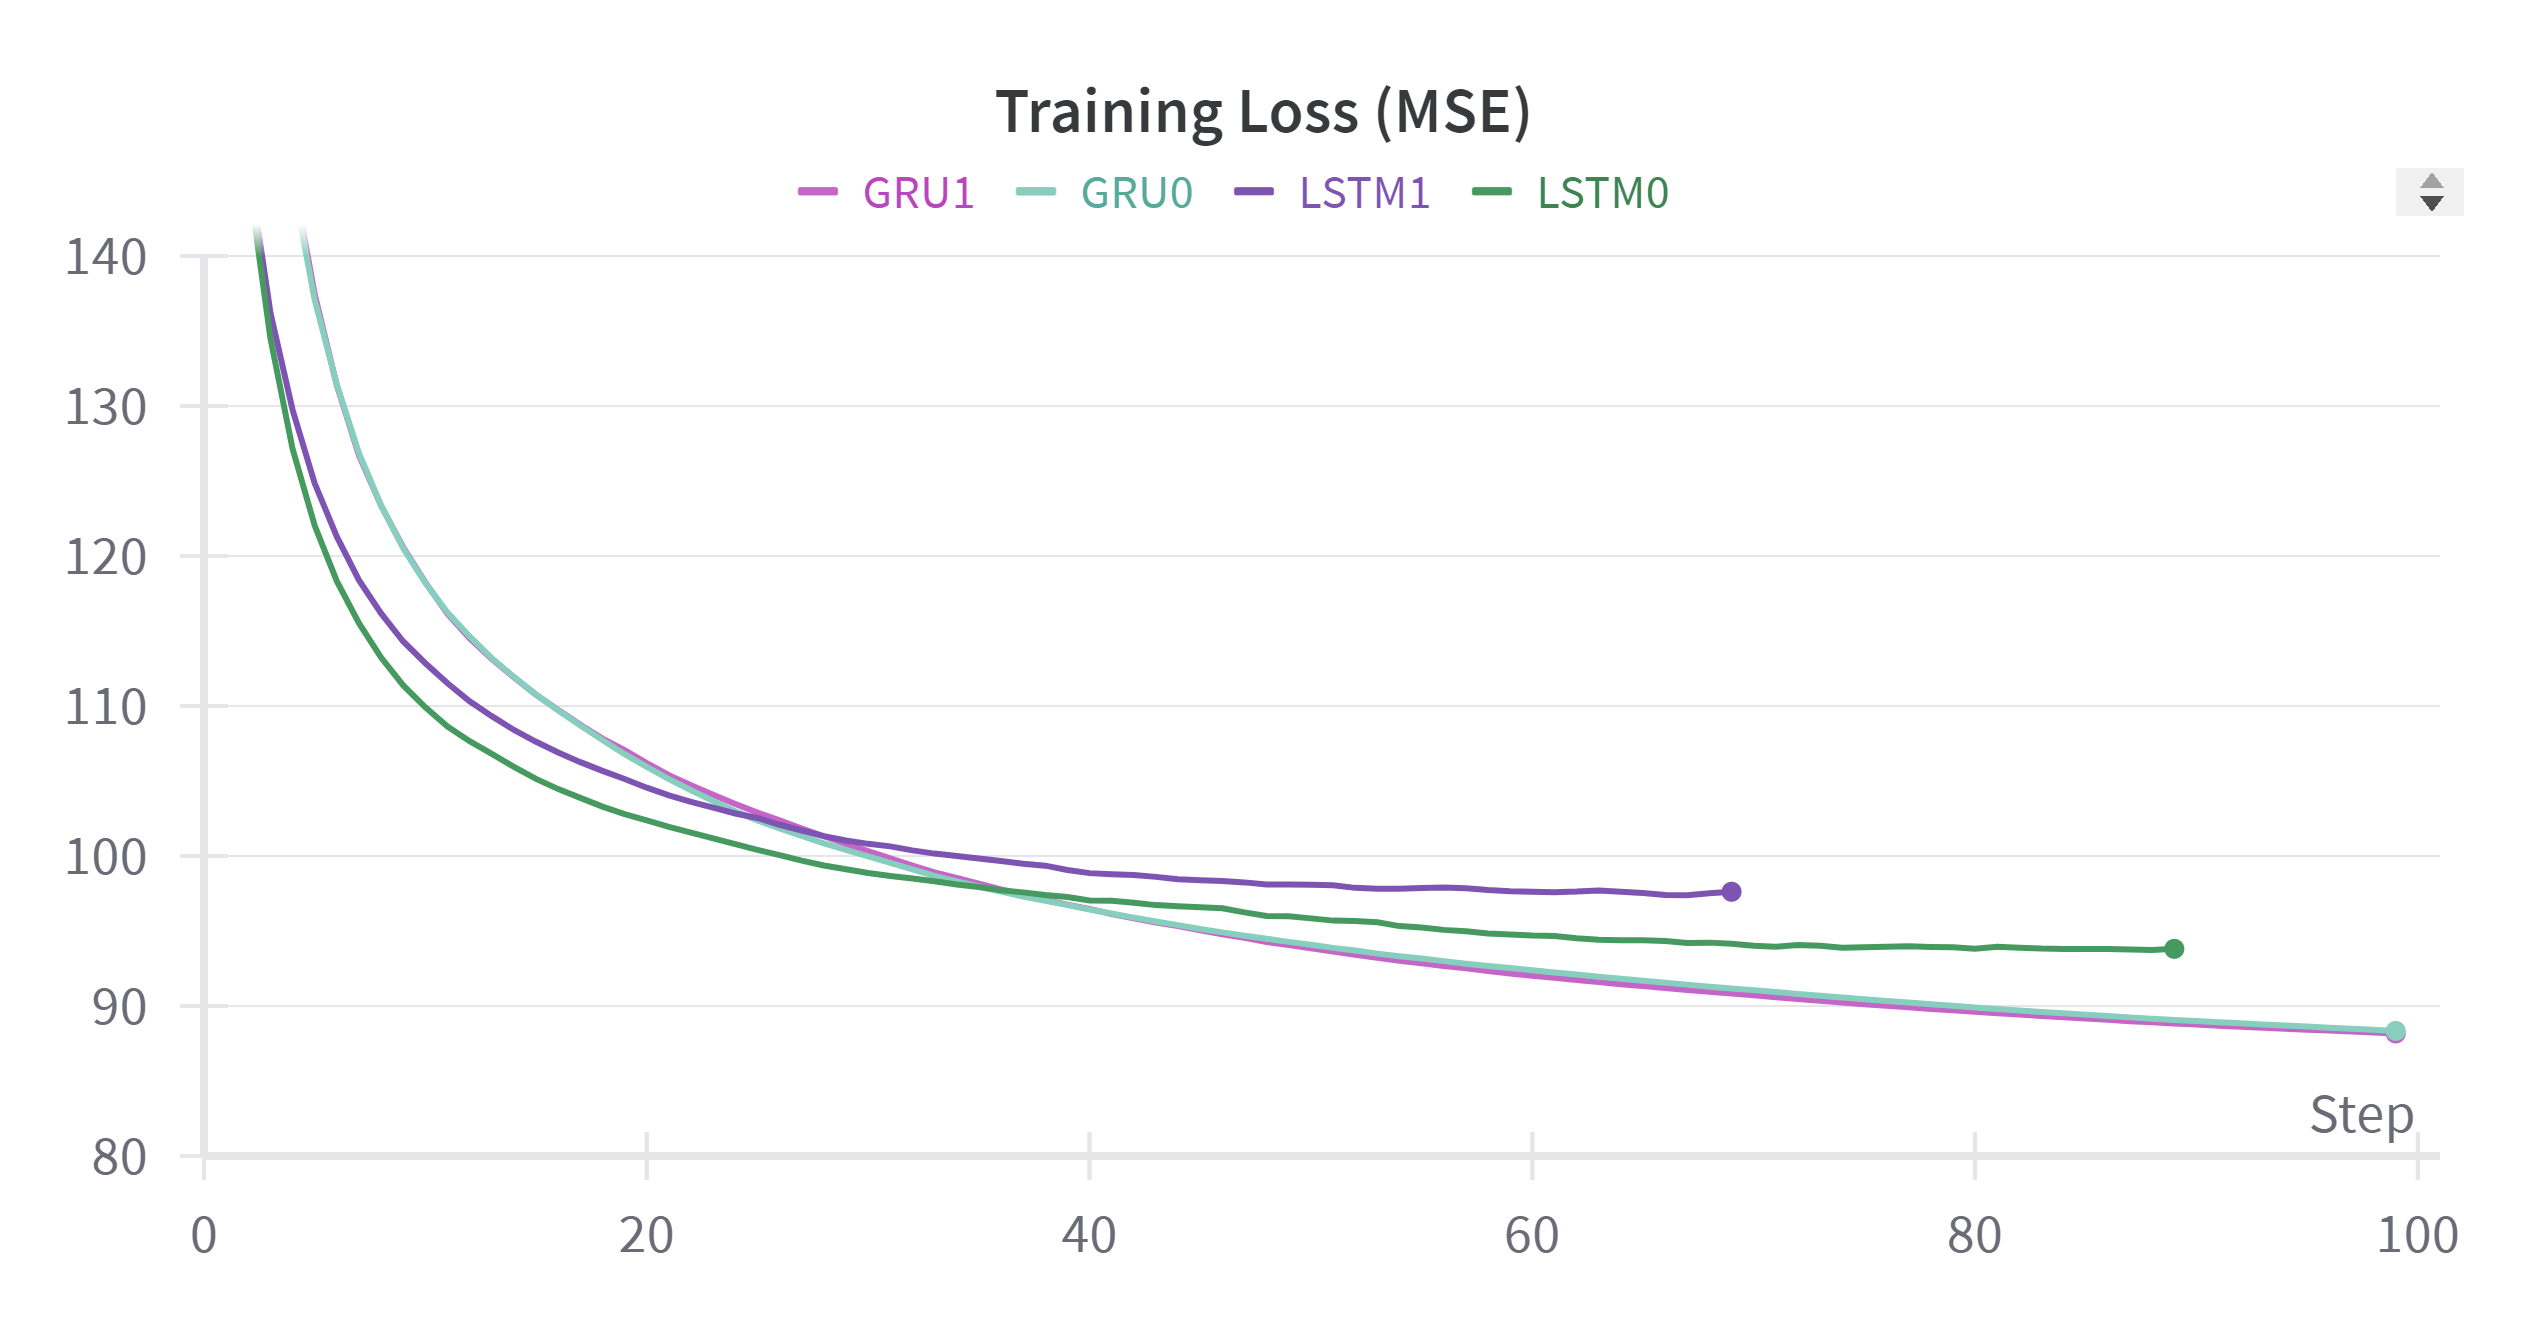
\includegraphics[width=0.4\linewidth]{images/results/LSTM_GRU_Train_mse}
    \caption{LSTM \& GRU Train MSE}
    \label{fig:train_mse}
\end{figure}

\begin{figure}[h]
    \centering
    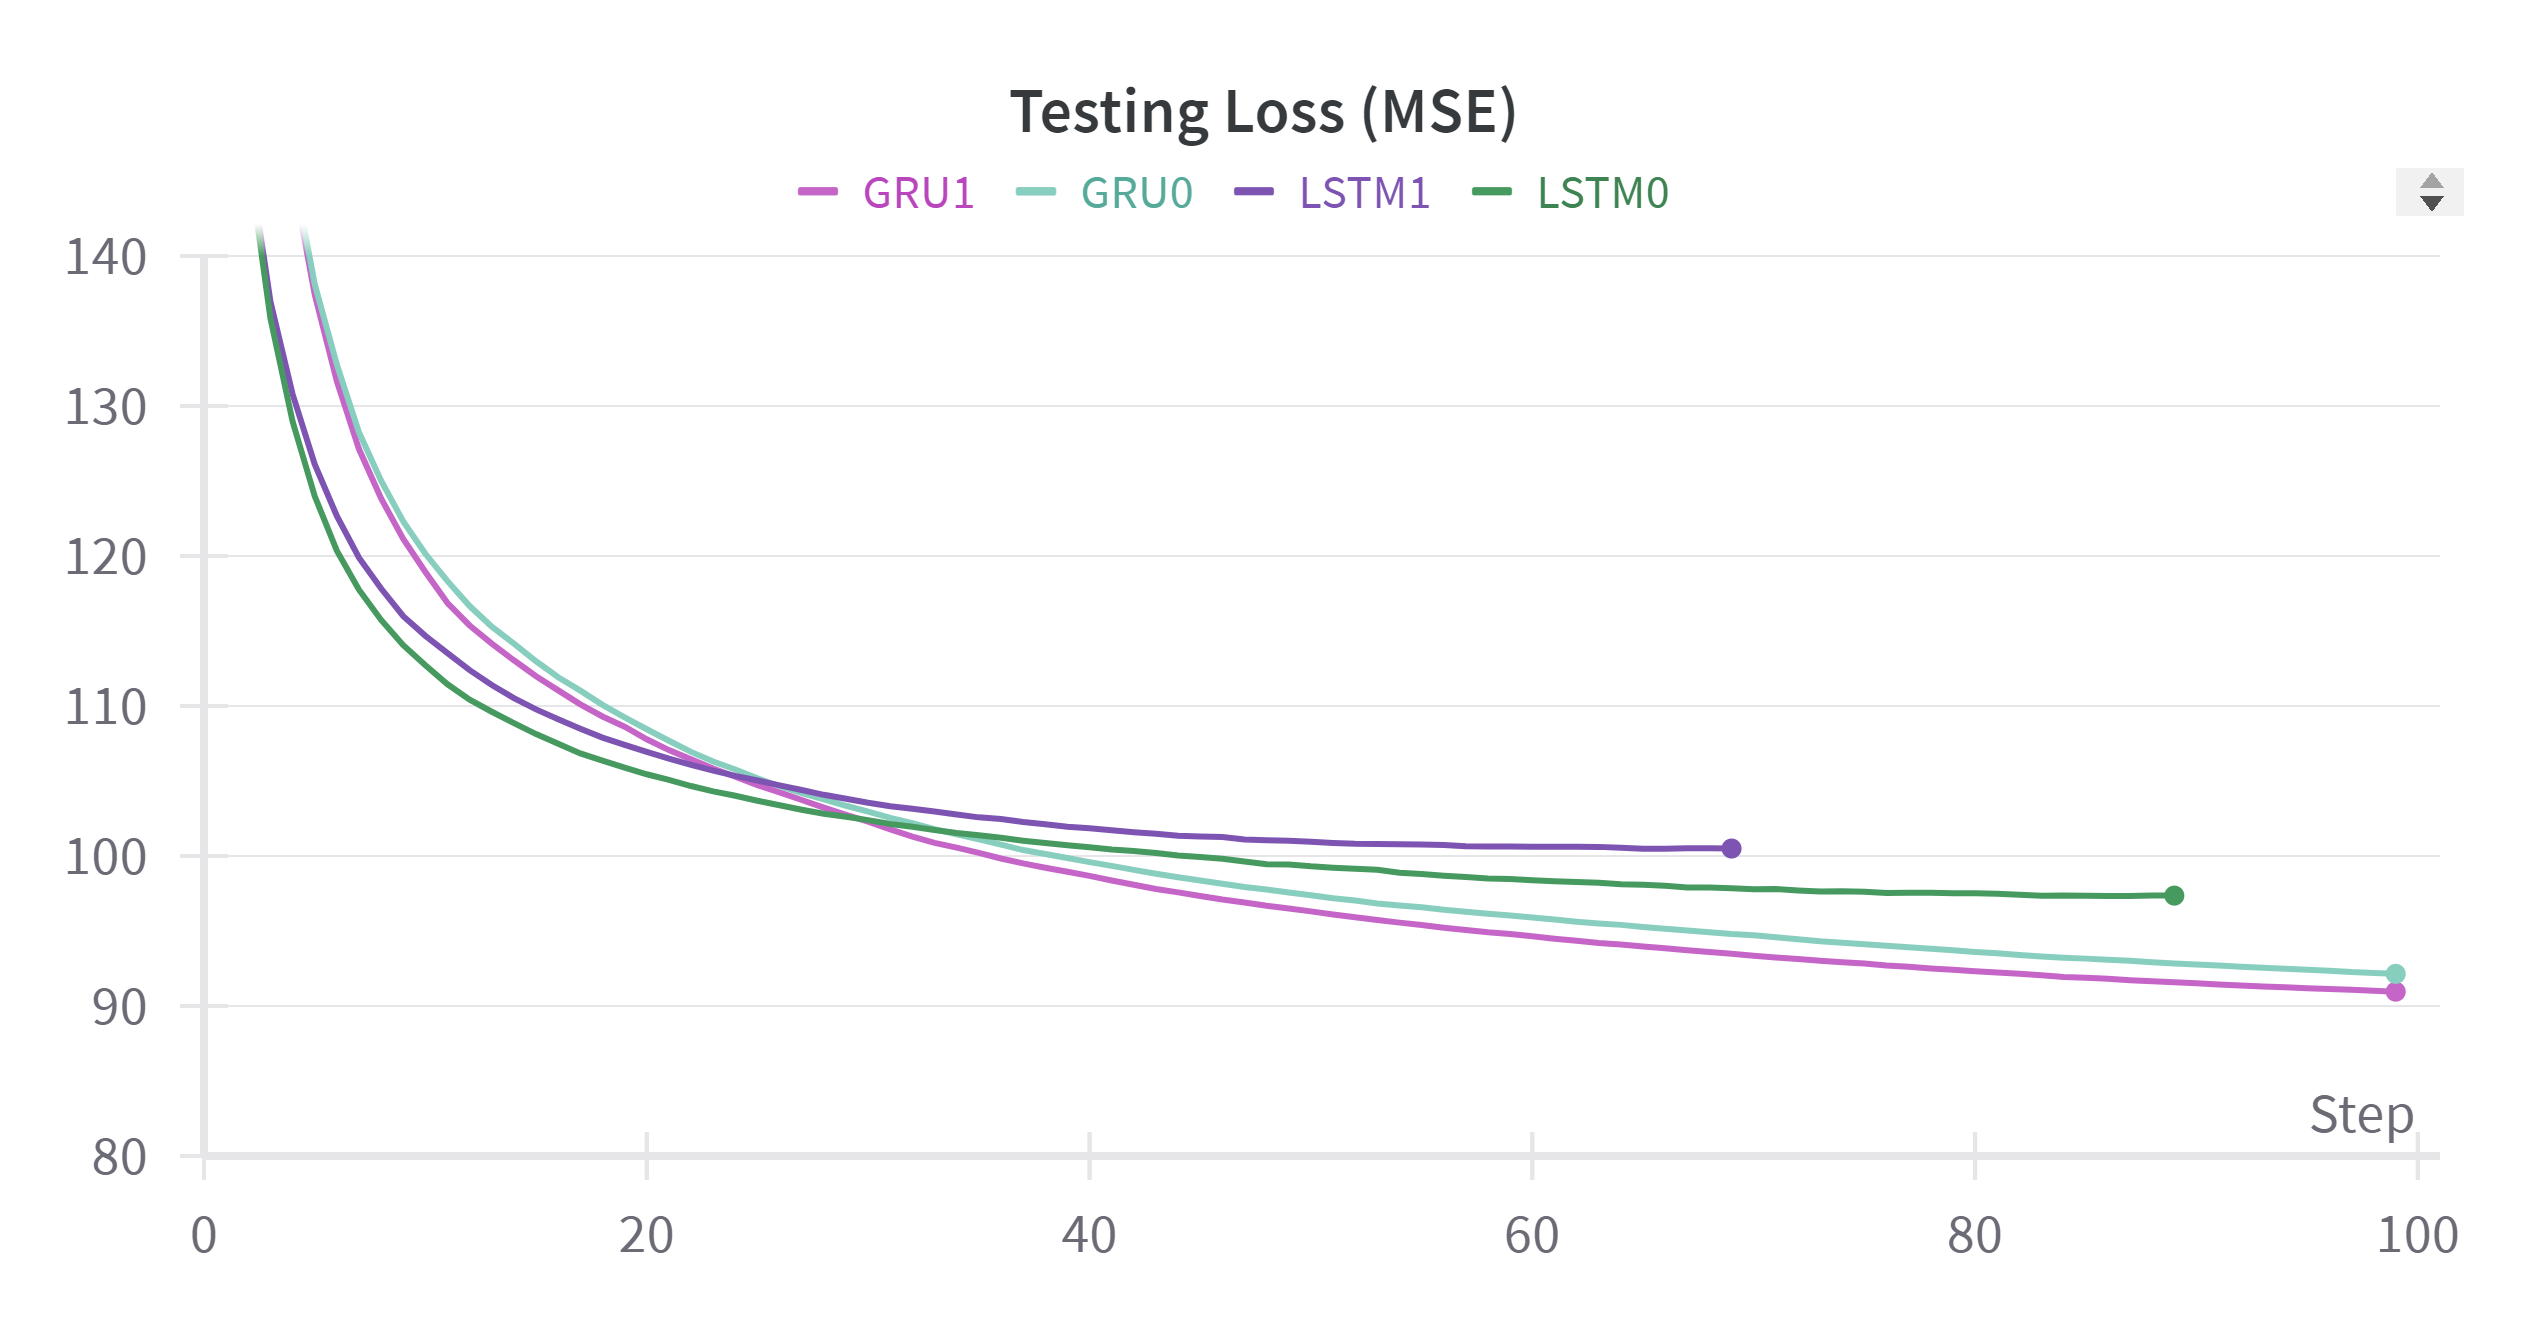
\includegraphics[width=0.4\linewidth]{images/results/LSTM_GRU_Test_mse}
    \caption{LSTM \& GRU Test MSE}
    \label{fig:test_mse}
\end{figure}

\begin{figure}[h]
    \centering
    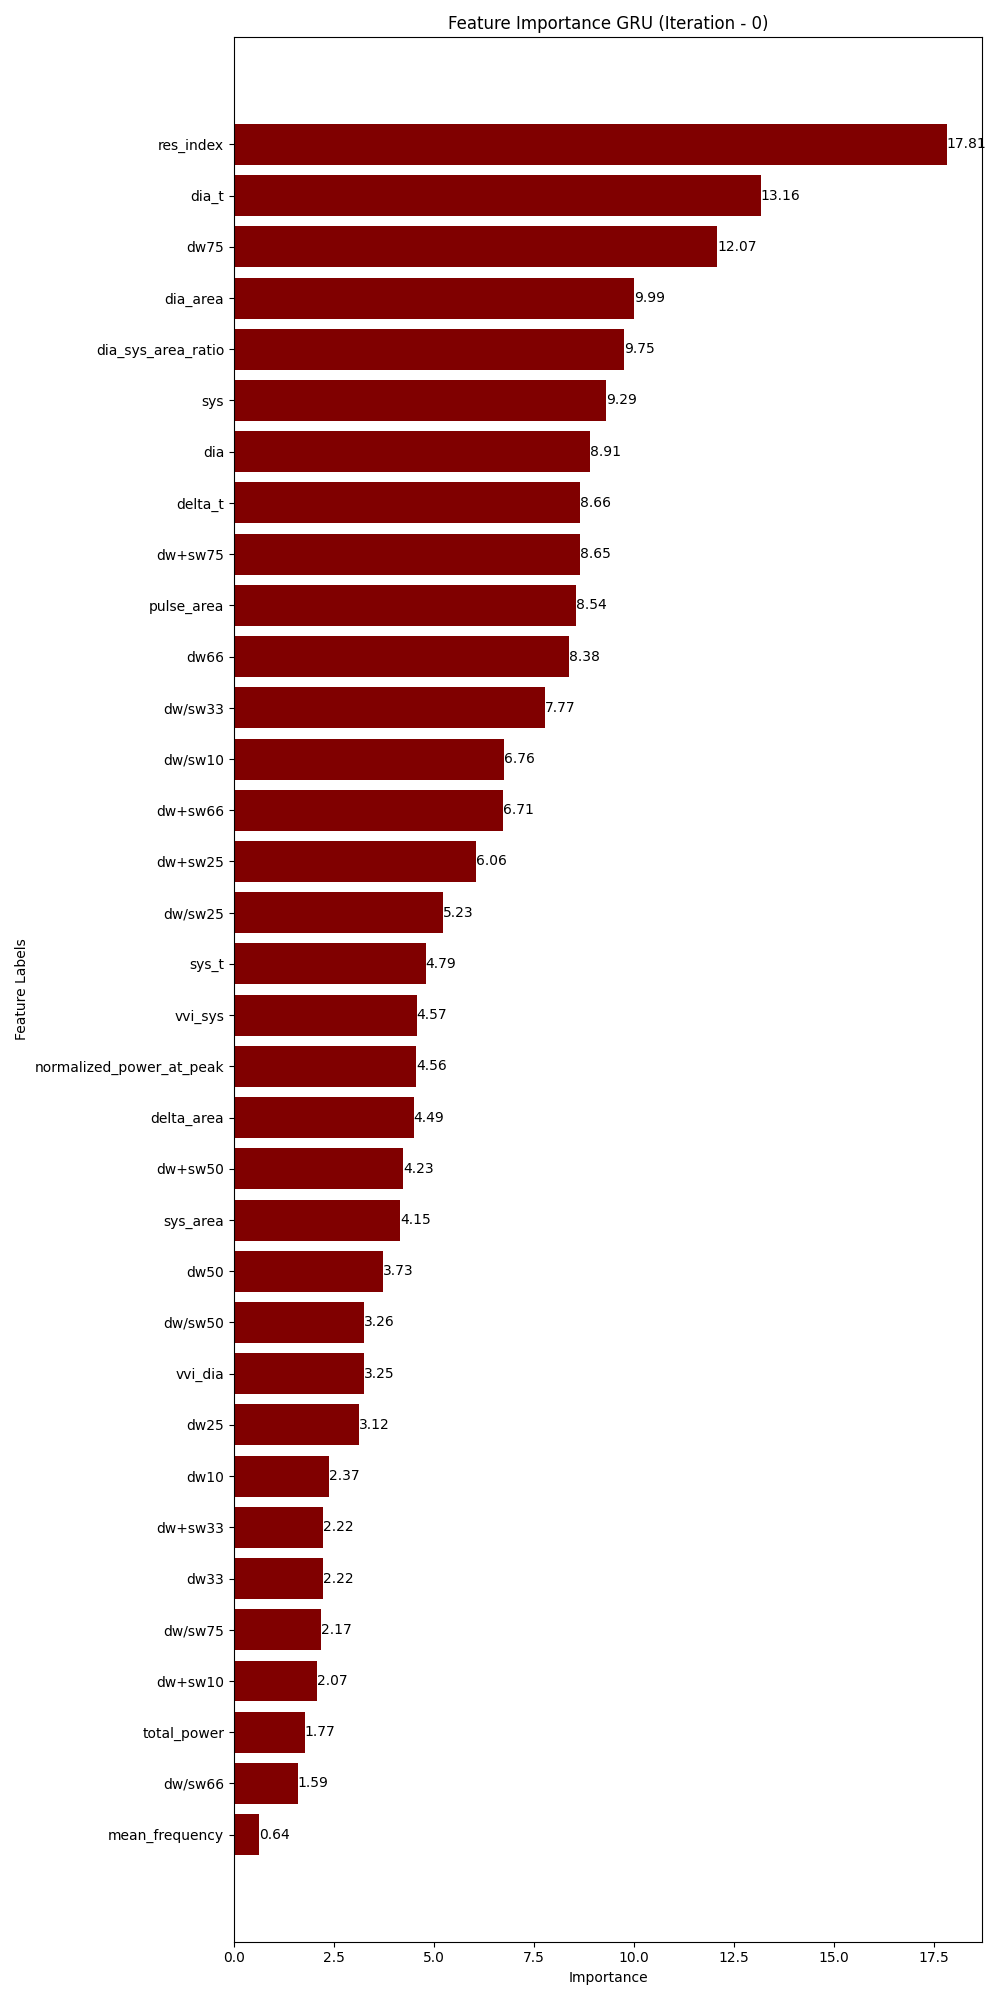
\includegraphics[width=0.5\textwidth]{images/results/feature_importance_plot_GRU_0}
    \caption{Feature Importance Chart}
    \label{fig:feat_importance}
\end{figure}



    \section{Discussion}
    \label{sec:discussion}

    Caveats:
    \begin{itemize}
        \item Out of the 34 features, 3 (delta\_t, delta\_area and res\_index) depend on the accurate detection of the dicrotic notch.
        \item Significantly more values could be extracted if finding the dicrotic notch would not be necessary.
    \end{itemize}

    % more effi sp for mimic3
    All this means is that the signal processing algorithms worked better and extracted more values from the MIMIC-III DB.
    It is also possible a hint at the fact, that the quality of the signal was better in MIMIC-III.
    This is also logical however, since there was no limit on the fetching of records from a single study or subject from MIMIC-IV,
    so huge number of segments might have been discarded, if they didn't showcase a comprehensible signal.

    % feature reduction
    It was found, that every feature contributes positively, therefore feature reduction was not applied.

    Limitations:
    \begin{itemize}
        \item Not knowing what devices were used.
        \item How they were calibrated.
        \item How accurate they are.
        \item Pulse oximeter and arterial catheter parameters.
        \item Sampling rates are different for every device (even between MIMIC 3 and 4).
    \end{itemize}

    Possible Improvements:
    \begin{itemize}
        \item Integrate both the ECG and PPG graphs for a more precise prediction.
        \item Use further signal processing approaches.
        \item Manually filter waveform graphics (e.g., faulty PPG signal).
        \item Expand on machine learning algorithms.
        \item Experiment with different median intervals.
        \item Experiment with further data splitting approaches.
    \end{itemize}


    \section{Conclusion}
    \label{sec:conclusion}

    Summary of findings:

    As per the joint 2018 statement by the American National Standards of the Association for the Advancement of Medical Instrumentation (AAMI), European Society of Hypertension (ESH)
    and International Organization for Standardization (ISO), the average variation and its standard deviation in NIBP measurements should ideally fall within 5 ± 8 mmHg compared to a reference BP,
    based on a minimum of 85 patient evaluations~\cite{stergiouUniversalStandardValidation2018}.

    The number of patient evaluations done in this study greatly exceed 85.
    The average variation and standard deviation of given models was: -||-

    Pretty bad performance on a huge number of data.
    Very important though, that no overfitting was done.
    Also, real-world data was simulated through MIMIC-IV (completely different data source), which is key.

    Advanced NN models performed well but not extraordinarily great.
    RF had a promising test loss, but validation loss was even worse than of LSTMs and GRUs.

    This study focused on ICU patient data, but it can prospectively be expanded on also ambulatory patients or even real-time healthy patient monitoring.

    \newpage

    \singlespacing
    \small
    \bibliographystyle{ieeetr}  % ieeetr
    \bibliography{literature_final_with_notes}
    \normalsize

    \newpage
    \appendix


    \section{Code}\label{sec:code}
    \subsection{Filters}\label{subsec:code_filters}

\begin{lstlisting}[language=Python,label={lst:filters.py}, basicstyle=\scriptsize]

from scipy.ndimage import gaussian_filter1d
import scipy as sp
import matplotlib.pyplot as plt
import numpy as np


def pre_process_data(abp, ppg, fs):
    # Gaussian filter
    g_abp = gaussian_filter1d(abp, sigma=2)
    g_ppg = gaussian_filter1d(ppg, sigma=2)

    # Gaussian Median filter
    med_a = np.median(abp)
    std_a = np.std(abp)
    sigma_a = med_a / std_a * 0.5
    gm_abp = gaussian_filter1d(abp, sigma=sigma_a)
    med_p = np.median(ppg)
    std_p = np.std(ppg)
    sigma_p = med_p / std_p * 0.3
    gm_ppg = gaussian_filter1d(ppg, sigma=sigma_p)

    # Savitzky-Golay filter
    sg_abp = filter_savgol(abp)
    sg_ppg = filter_savgol(ppg)

    # Butterworth Lowpass filter
    bl_abp = butter_lowpass_filter(abp, 5, fs, 4)
    bl_ppg = butter_lowpass_filter(ppg, 5, fs, 4)

    # Butterworth filter
    b_abp = filter_butterworth(abp, fs)
    b_ppg = filter_butterworth(ppg, fs)

    # Chebyshev Lowpass filter
    cl_abp = chebyshev2_lowpass_filter(abp, 2, fs)
    cl_ppg = chebyshev2_lowpass_filter(ppg, 2, fs)

    # Chebyshev filter
    c_abp = filter_chebyshev(abp, fs)
    c_ppg = filter_chebyshev(ppg, fs)

    # Whiskers filter
    w_abp = whiskers_filter(abp)
    w_ppg = whiskers_filter(ppg)


def filter_savgol(x):
    x_f = sp.savgol_filter(x, 51, 4)
    return x_f


def butter_lowpass_filter(data, cutoff_frequency, fs, order):
    nyquist = 0.5 * fs
    normal_cutoff = cutoff_frequency / nyquist
    b, a = sp.butter(order, normal_cutoff, btype='low', analog=False, output='ba')

    filtered_data = sp.lfilter(b, a, data)
    return filtered_data


def chebyshev2_lowpass_filter(data, cutoff_freq, fs):
    nyquist = 0.5 * fs
    normal_cutoff = cutoff_freq / nyquist
    b, a = sp.cheby2(4, 2, normal_cutoff, btype='low', analog=False)
    y = sp.lfilter(b, a, data)
    return y


def filter_butterworth(data, fs):
    lpf_cutoff = 1.25  # Hz
    hpf_cutoff = 31  # Hz
    sos_butt = sp.butter(10,
                         [lpf_cutoff, hpf_cutoff],
                         btype='bp',
                         analog=False,
                         output='sos',
                         fs=fs)
    w, h = sp.sosfreqz(sos_butt,
                       2000,
                       fs=fs)
    sos = sos_butt, w, h
    return sp.sosfiltfilt(sos[0], data)


def filter_chebyshev(data, fs):
    lpf_cutoff = 1.2  # Hz
    hpf_cutoff = 60  # Hz
    sos_cheb = sp.cheby2(4,
                         20,
                         [lpf_cutoff, hpf_cutoff],
                         btype='bp',
                         analog=False,
                         output='sos',
                         fs=fs)
    w, h = sp.sosfreqz(sos_cheb,
                       2000,
                       fs=fs)
    sos = sos_cheb, w, h
    return sp.sosfiltfilt(sos[0], data)


def whiskers_filter(data):
    bp = plt.boxplot(data)
    plt.close()

    # get lower and upper amplitude thresholds
    whiskers = [whiskers.get_ydata() for whiskers in bp['whiskers']]
    lower_amp = whiskers[0][1]
    upper_amp = whiskers[1][1]

    # get all indexes of outliers, outside the amplitude thresholds
    ind_outliers = []
    for i in range(len(data)):
        if data[i] < lower_amp or data[i] > upper_amp:
            ind_outliers.append(i)

    if len(ind_outliers) != 0:
        # get all grouped arrays with values not within the whiskers range
        ind_consecutives = []
        current_group = [ind_outliers[0]]
        for i in range(1, len(ind_outliers)):
            if ind_outliers[i] == ind_outliers[i - 1] + 1:
                current_group.append(ind_outliers[i])
            else:
                ind_consecutives.append(current_group)
                current_group = [ind_outliers[i]]
        ind_consecutives.append(current_group)

        for array_indexes in ind_consecutives:
            array_values = data[array_indexes]
            # get top (min or max) value of each consecutive group
            if array_values[0] < lower_amp:
                top_val = min(array_values)
                top_ind = array_indexes[np.argmin(array_values)]
                coef = top_val / lower_amp
            else:
                top_val = max(array_values)
                top_ind = array_indexes[np.argmax(array_values)]
                coef = top_val / upper_amp
            # calculate and (not) assign the top value according to attenuating coefficient
            adj_top_val = top_val / coef * 1.01
            if lower_amp > top_val > adj_top_val:
                continue
            if upper_amp < top_val < adj_top_val:
                continue
            data[top_ind] = adj_top_val
            # check if first group index is also first overall index
            if array_indexes[0] == 0:
                one_minus_threshold_val = data[array_indexes[0]]
                one_minus_threshold_ind = array_indexes[0]
            else:
                one_minus_threshold_val = data[array_indexes[0] - 1]
                one_minus_threshold_ind = array_indexes[0] - 1
            # check if last group index is also last overall index
            if array_indexes[-1] == len(data) - 1:
                one_plus_threshold_val = data[array_indexes[-1]]
                one_plus_threshold_ind = array_indexes[-1]
            else:
                one_plus_threshold_val = data[array_indexes[-1] + 1]
                one_plus_threshold_ind = array_indexes[-1] + 1
            # create function for calculation of other new values
            distance_to_top = top_ind - one_minus_threshold_ind
            if distance_to_top == 0:
                distance_to_top = 1
            distance_to_bottom = one_plus_threshold_ind - top_ind
            if distance_to_bottom == 0:
                distance_to_bottom = 1
            f1 = (adj_top_val - one_minus_threshold_val) / distance_to_top
            f2 = (one_plus_threshold_val - adj_top_val) / distance_to_bottom
            # assign new values
            x1, x2 = 1, 1
            for ind in array_indexes:
                if ind < top_ind:
                    data[ind] = (f1 * x1) + one_minus_threshold_val
                    x1 += 1
                elif ind > top_ind:
                    data[ind] = (f2 * x2) + adj_top_val
                    x2 += 1

    return data

\end{lstlisting}

\newpage

\subsection{Beats}
\label{subsec:code_beats}

\begin{lstlisting}[language=Python,label={lst:beats.py}, basicstyle=\scriptsize]
import scipy as sp
import numpy as np


def get_optimal_beats_lists(abp, ppg, fs):
    """
    Signal processing script for examining
    which default beat detection algorithm is the most efficient
    :param abp: List of ABP data
    :param ppg: List of PPG data
    :param fs: Sampling frequency
    :return: Lists of optimally detected ABP and PPG pulses
    """
    abp_beats1 = pulse_detection(abp, 'd2max', len(abp) / fs, 'abp')
    ppg_beats1 = pulse_detection(ppg, 'd2max', len(ppg) / fs, 'ppg')
    abp_beats2 = pulse_detection(abp, 'upslopes', len(abp) / fs, 'abp')
    ppg_beats2 = pulse_detection(ppg, 'upslopes', len(ppg) / fs, 'ppg')
    abp_beats3 = pulse_detection(abp, 'delineator', len(abp) / fs, 'abp')
    ppg_beats3 = pulse_detection(ppg, 'delineator', len(ppg) / fs, 'ppg')

    avg1 = (len(abp_beats1) + len(ppg_beats1)) / 2
    avg2 = (len(abp_beats2) + len(ppg_beats2)) / 2
    avg3 = (len(abp_beats3) + len(ppg_beats3)) / 2

    sorted_avg = sorted([avg1, avg2, avg3])
    diff_avg12 = sorted_avg[1] - sorted_avg[0]
    diff_avg23 = sorted_avg[2] - sorted_avg[1]

    outlier = None
    if diff_avg23 > diff_avg12 * 2:
        outlier = sorted_avg[2]
    elif diff_avg12 > diff_avg23 * 2:
        outlier = sorted_avg[0]

    diff1 = abs(len(abp_beats1) - len(ppg_beats1))
    diff2 = abs(len(abp_beats2) - len(ppg_beats2))
    diff3 = abs(len(abp_beats3) - len(ppg_beats3))

    diffper1 = diff1 / avg1 * 100
    diffper2 = diff2 / avg2 * 100
    diffper3 = diff3 / avg3 * 100

    if outlier is None:
        abp_opt, ppg_opt = get_best_beats_from_diffper(diffper1, diffper2, diffper3,
                                                       abp_beats1, abp_beats2, abp_beats3,
                                                       ppg_beats1, ppg_beats2, ppg_beats3)
    else:
        if outlier == avg1:
            diffper1 = 100
        elif outlier == avg2:
            diffper2 = 100
        elif outlier == avg3:
            diffper3 = 100
        abp_opt, ppg_opt = get_best_beats_from_diffper(diffper1, diffper2, diffper3,
                                                   abp_beats1, abp_beats2, abp_beats3,
                                                   ppg_beats1, ppg_beats2, ppg_beats3)
    return abp_opt, ppg_opt


def pulse_detection(data, algorithm, duration):
    temp_fs = 125
    beats = pulse_detect(data, temp_fs, 5, algorithm, duration)
    return beats


def get_best_beats_from_diffper(diffper1, diffper2, diffper3,
                                abp_beats1, abp_beats2, abp_beats3,
                                ppg_beats1, ppg_beats2, ppg_beats3):
    smallest_diffper = min(diffper1, diffper2, diffper3)

    abp_opt = []
    ppg_opt = []

    if smallest_diffper == diffper1:
        abp_opt = abp_beats1
        ppg_opt = ppg_beats1
    elif smallest_diffper == diffper2:
        abp_opt = abp_beats2
        ppg_opt = ppg_beats2
    elif smallest_diffper == diffper3:
        abp_opt = abp_beats3
        ppg_opt = ppg_beats3

    return abp_opt, ppg_opt

def pulse_detect(x, fs, w, alg, dur):
    """
    Description: Pulse detection and correction from pulsatile signals
    Developed by: Elisa Mejia-Mejia
                   City, University of London
    Full code available at:
    https://wfdb.io/mimic_wfdb_tutorials/tutorial/notebooks/beat-detection.html
    """


def get_beats_from_mean_crossings(abp, ppg):
    mean_value = np.mean(abp)
    above_mean = abp > mean_value
    count_a = np.count_nonzero(np.diff(above_mean.astype(int)) == -1)
    mean_value = np.mean(ppg)
    above_mean = ppg > mean_value
    count_p = np.count_nonzero(np.diff(above_mean.astype(int)) == -1)
    abp_beat_interval = len(abp) / ((count_a + count_p) / 2)
    ppg_beat_interval = abp_beat_interval

    abp_beats, _ = sp.find_peaks(abp, distance=abp_beat_interval, prominence=5)
    ppg_beats, _ = sp.find_peaks(ppg, distance=ppg_beat_interval, prominence=0.01)

    return abp_beats, ppg_beats

\end{lstlisting}

\newpage

\subsection{Signal Processing}
\label{subsec:code_sp}

\begin{lstlisting}[language=Python,label={lst:sp.py}, basicstyle=\scriptsize]
import numpy as np
import scipy as sp


def signal_processing(seg_name, abp, ppg, fs):
    # First iteration of beat finding (MIMIC default methods)
    abp_beats, ppg_beats = get_optimal_beats_lists(abp, ppg, seg_name)

    # For comparison: beat detection from mean crossing
    beats_a, beats_p = get_beats_from_mean_crossings(abp, ppg)
    is_larger = len(beats_a) + len(beats_p) > len(abp_beats) + len(beats_p)
    is_closer = abs(len(beats_a) - len(beats_p)) < abs(len(abp_beats) - len(ppg_beats))
    if is_larger and is_closer:
        abp_beats = beats_a
        ppg_beats = beats_p

    # Second iteration: Peak finding (SP manual methods)
    abp_beat_interval = len(abp) / len(abp_beats)
    ppg_beat_interval = len(ppg) / len(ppg_beats)
    abp_beats, _ = sp.find_peaks(abp, distance=abp_beat_interval * .75, prominence=0.5)
    ppg_beats, _ = sp.find_peaks(ppg, distance=ppg_beat_interval * .75, prominence=0.01)
    if len(abp_beats) < 100 or len(ppg_beats) < 100:
        raise Exception('Signal Processing failed: a substantial amount of beats not found')

    # Signal synchronization : delay approx = 18 (288 ms)
    abp, ppg = synchronization(abp, ppg, abp_beats, ppg_beats)

    # Third iteration: Peak finding
    abp_beats, _ = sp.find_peaks(abp, distance=abp_beat_interval * .75, prominence=0.5)
    ppg_beats, _ = sp.find_peaks(ppg, distance=ppg_beat_interval * .75, prominence=0.01)
    normal_length_a, normal_length_p = len(abp_beats), len(ppg_beats)

    # Beat grouping
    abp_beats, ppg_beats = group_beats(abp_beats, ppg_beats)

    if max(normal_length_a, normal_length_p) > max(len(abp_beats), len(ppg_beats)) * 1.05:
        raise Exception(f"too big of a difference after grouping -"
                        f"{max(normal_length_a,normal_length_p)-max(len(abp_beats),len(ppg_beats))}")

    abp_hr = round(len(abp_beats) / (len(abp) / fs) * 60, 1)
    ppg_hr = round(len(ppg_beats) / (len(ppg) / fs) * 60, 1)
    print(f"\tABP beats - {len(abp_beats)}, Heart Rate - {abp_hr}")
    print(f"\tPPG beats - {len(ppg_beats)}, Heart Rate - {ppg_hr}")

    return {
        'abp': abp,
        'ppg': ppg,
        'abp_beats': abp_beats,
        'ppg_beats': ppg_beats,
        'abp_hr': abp_hr,
        'ppg_hr': ppg_hr
    }


def synchronization(abp, ppg, abp_beats, ppg_beats):
    # Find closest PPG beat to first ABP beat
    first_ppg_ind, first_abp = None, None
    for i in range(0, len(abp_beats)):
        first_abp = abp_beats[i]
        differences = ppg_beats - first_abp
        arr = [num for num in differences if num > 0]
        if len(arr) == 0:
            raise Exception("Beat synchronisation failed: no proximal beats found")
        smallest_diff = min(arr)
        if smallest_diff < 50:
            first_ppg_ind, = np.argwhere(differences == smallest_diff)[0]
            break
    first_ppg = ppg_beats[first_ppg_ind]

    # Find closest ABP beat to last PPG beat
    last_ppg_ind = len(ppg_beats) - 1
    last_ppg = ppg_beats[last_ppg_ind]
    differences = abs(abp_beats - last_ppg)
    last_abp_ind = np.argmin(differences)
    last_abp = abp_beats[last_abp_ind]

    # Splice original ABP and PPG arrays
    new_abp = abp[first_abp:last_abp]
    new_ppg = ppg[first_ppg:last_ppg]

    return new_abp, new_ppg


def group_beats(abp_beats, ppg_beats):
    i = 0
    while i < min(len(abp_beats), len(ppg_beats)):
        a = abp_beats[i]
        p = ppg_beats[i]
        if p - 40 <= a <= p + 40:
            i += 1
        else:
            if a < p:
                abp_beats = abp_beats[abp_beats != a]
            elif a > p:
                ppg_beats = ppg_beats[ppg_beats != p]
    abp_beats, ppg_beats = equal_out_by_shortening(abp_beats, ppg_beats)
    return abp_beats, ppg_beats


def equal_out_by_shortening(a_ts, p_ts):
    if len(a_ts) > len(p_ts):
        diff = len(a_ts) - len(p_ts)
        a_ts = a_ts[:-diff]
    elif len(a_ts) < len(p_ts):
        diff = len(p_ts) - len(a_ts)
        p_ts = p_ts[:-diff]
    return a_ts, p_ts
\end{lstlisting}

\newpage

\subsection{Fiducial Points}
\label{subsec:code_fidp}

\begin{lstlisting}[language=Python,label={lst:fidp.py}, basicstyle=\scriptsize]
import numpy as np
import scipy as sp


def fiducial_points(x, pks, fs, vis, header):
    """
    Description: Pulse detection and correction from pulsatile signals
    Inputs:  x, array with pulsatile signal [user defined units]
             pks, array with the position of the peaks [number of samples]
             fs, sampling rate of signal [Hz]
             vis, visualisation option [True, False]
    Outputs: fidp, dictionary with the positions of several fiducial points
             for the cardiac cycles [number of samples]

    Fiducial points:  1: Systolic peak (pks)
                      2: Onset, as the minimum before the systolic peak (ons)
                      3: Onset, using the tangent intersection method (ti)
                      4: Diastolic peak (dpk)
                      5: Maximum slope (m1d)
                      6: a point from second derivative PPG (a2d)
                      7: b point from second derivative PPG (b2d)
                      8: c point from second derivative PPG (c2d)
                      9: d point from second derivative PPG (d2d)
                      10: e point from second derivative PPG (e2d)
                      11: p1 from the third derivative PPG (p1)
                      12: p2 from the third derivative PPG (p2)

    Libraries: NumPy (as np), SciPy (Signal, as sp), Matplotlib (PyPlot, as plt)

    Version: 1.0 - June 2022

    Developed by: Elisa Mejia-Mejia
                   City, University of London

    Edited by: Peter Charlton (see "Added by PC"), Hugas Jasinskas (see "Adjusted by HJ")

    """
    # First, second and third derivatives
    d1x = sp.savgol_filter(x, 9, 5, deriv=1)
    d2x = sp.savgol_filter(x, 9, 5, deriv=2)
    d3x = sp.savgol_filter(x, 9, 5, deriv=3)

    # Search in time series: Onsets between consecutive peaks
    ons = np.empty(0)
    for i in range(len(pks) - 1):
        start = pks[i]
        stop = pks[i + 1]
        ibi = x[start:stop]
        aux_ons, = np.where(ibi == np.min(ibi))
        if len(aux_ons) > 1:
            aux_ons = aux_ons[0]
        ind_ons = aux_ons.astype(int)
        ons = np.append(ons, ind_ons + start)
    ons = ons.astype(int)

    # Search in time series: Diastolic peak and dicrotic notch between consecutive onsets
    dia = np.empty(0)
    dic = np.empty(0)
    for i in range(len(ons) - 1):
        start = ons[i]
        stop = ons[i + 1]
        ind_pks, = np.intersect1d(np.where(pks < stop), np.where(pks > start))
        ind_pks = pks[ind_pks]
        ibi_portion = x[ind_pks:stop]
        ibi_2d_portion = d2x[ind_pks:stop]
        aux_dic, _ = sp.find_peaks(ibi_2d_portion)
        aux_dic = aux_dic.astype(int)
        aux_dia, _ = sp.find_peaks(-ibi_2d_portion)
        aux_dia = aux_dia.astype(int)
        if len(aux_dic) != 0:
            ind_max, = np.where(ibi_2d_portion[aux_dic] == np.max(ibi_2d_portion[aux_dic]))
            aux_dic_max = aux_dic[ind_max][0]  # Adjusted by HJ
            if len(aux_dia) != 0:
                nearest = aux_dia - aux_dic_max
                aux_dic = aux_dic_max
                dic = np.append(dic, (aux_dic + ind_pks).astype(int))
                ind_dia, = np.where(nearest > 0)
                aux_dia = aux_dia[ind_dia]
                nearest = nearest[ind_dia]
                if len(nearest) != 0:
                    ind_nearest, = np.where(nearest == np.min(nearest))
                    aux_dia = aux_dia[ind_nearest]
                    dia = np.append(dia, (aux_dia + ind_pks).astype(int))
            else:
                dic = np.append(dic, (aux_dic_max + ind_pks).astype(int))
    dia = dia.astype(int)
    dic = dic.astype(int)

    # Search in D1: Maximum slope point
    m1d = np.empty(0)
    for i in range(len(ons) - 1):
        start = ons[i]
        stop = ons[i + 1]
        ind_pks, = np.intersect1d(np.where(pks < stop), np.where(pks > start))
        ind_pks = pks[ind_pks]
        ibi_portion = x[start:ind_pks]
        ibi_1d_portion = d1x[start:ind_pks]
        aux_m1d, _ = sp.find_peaks(ibi_1d_portion)
        aux_m1d = aux_m1d.astype(int)
        if len(aux_m1d) != 0:
            ind_max, = np.where(ibi_1d_portion[aux_m1d] == np.max(ibi_1d_portion[aux_m1d]))
            aux_m1d_max = aux_m1d[ind_max]
            if len(aux_m1d_max) > 1:
                aux_m1d_max = aux_m1d_max[0]
            m1d = np.append(m1d, (aux_m1d_max + start).astype(int))
    m1d = m1d.astype(int)

    # Search in time series: Tangent intersection points
    tip = np.empty(0)
    for i in range(len(ons) - 1):
        start = ons[i]
        stop = ons[i + 1]
        ibi_portion = x[start:stop]
        ibi_1d_portion = d1x[start:stop]
        low_stop = np.where(m1d < stop)  # Adjusted by HJ from here
        high_start = np.where(m1d > start)
        if np.intersect1d(low_stop, high_start).size == 0:
            continue
        ind_m1d, = np.intersect1d(low_stop, high_start)  # to here
        ind_m1d = m1d[ind_m1d] - start
        aux_tip = np.round(((ibi_portion[0] - ibi_portion[ind_m1d]) /
                             ibi_1d_portion[ind_m1d]) + ind_m1d)
        aux_tip = aux_tip.astype(int)
        tip = np.append(tip, (aux_tip + start).astype(int))
    tip = tip.astype(int)

    # Search in D2: A, B, C, D and E points
    a2d = np.empty(0)
    b2d = np.empty(0)
    c2d = np.empty(0)
    d2d = np.empty(0)
    e2d = np.empty(0)
    for i in range(len(ons) - 1):
        start = ons[i]
        stop = ons[i + 1]
        ibi_portion = x[start:stop]
        ibi_1d_portion = d1x[start:stop]
        ibi_2d_portion = d2x[start:stop]
        ind_m1d = np.intersect1d(np.where(m1d > start), np.where(m1d < stop))
        ind_m1d = m1d[ind_m1d]
        aux_m2d_pks, _ = sp.find_peaks(ibi_2d_portion)
        aux_m2d_ons, _ = sp.find_peaks(-ibi_2d_portion)
        if len(aux_m2d_pks) == 0 or len(aux_m2d_ons) == 0:  # Augmented by HJ
            continue
        # a point:
        ind_a, = np.where(ibi_2d_portion[aux_m2d_pks] == np.max(ibi_2d_portion[aux_m2d_pks]))
        ind_a = aux_m2d_pks[ind_a]
        ind_a = ind_a[0]  # Adjusted by HJ
        if (ind_a < ind_m1d):
            a2d = np.append(a2d, ind_a + start)
            # b point:
            ind_b = np.where(ibi_2d_portion[aux_m2d_ons] == np.min(ibi_2d_portion[aux_m2d_ons]))
            ind_b = aux_m2d_ons[ind_b]
            ind_b = ind_b[0]  # Adjusted by HJ
            if (ind_b > ind_a) and (ind_b < len(ibi_2d_portion)):
                b2d = np.append(b2d, ind_b + start)
        # e point:
        if len(ind_m1d) == 0: # Augmented by HJ
            continue
        ind_e, = np.where(aux_m2d_pks > ind_m1d - start)
        aux_m2d_pks = aux_m2d_pks[ind_e]
        ind_e, = np.where(aux_m2d_pks < 0.6 * len(ibi_2d_portion))
        ind_e = aux_m2d_pks[ind_e]
        if len(ind_e) >= 1:
            if len(ind_e) >= 2:
                ind_e = ind_e[1]
            e2d = np.append(e2d, ind_e + start)
            # c point:
            ind_c, = np.where(aux_m2d_pks < ind_e)
            if len(ind_c) != 0:
                ind_c_aux = aux_m2d_pks[ind_c]
                ind_c, = np.where(ibi_2d_portion[ind_c_aux] == np.max(ibi_2d_portion[ind_c_aux]))
                ind_c = ind_c_aux[ind_c]
                if len(ind_c) != 0:
                    c2d = np.append(c2d, ind_c + start)
            else:
                aux_m1d_ons, _ = sp.find_peaks(-ibi_1d_portion)
                ind_c, = np.where(aux_m1d_ons < ind_e)
                ind_c_aux = aux_m1d_ons[ind_c]
                if len(ind_c) != 0:
                    ind_c, = np.where(ind_c_aux > ind_b)
                    ind_c = ind_c_aux[ind_c]
                    if len(ind_c) > 1:
                        ind_c = [ind_c[0]]  # Adjusted by HJ
                    c2d = np.append(c2d, ind_c + start)
            # d point:
            if len(ind_c) != 0:
                ind_d = np.intersect1d(np.where(aux_m2d_ons < ind_e), np.where(aux_m2d_ons > ind_c))
                if len(ind_d) != 0:
                    ind_d_aux = aux_m2d_ons[ind_d]
                    ind_d, = np.where(ibi_2d_portion[ind_d_aux] == np.min(ibi_2d_portion[ind_d_aux]))
                    ind_d = ind_d_aux[ind_d]
                    if len(ind_d) != 0:
                        d2d = np.append(d2d, ind_d + start)
                else:
                    ind_d = ind_c
                    d2d = np.append(d2d, ind_d + start)
    a2d = a2d.astype(int)
    b2d = b2d.astype(int)
    c2d = c2d.astype(int)
    d2d = d2d.astype(int)
    e2d = e2d.astype(int)

    # Search in D3: P1 and P2 points
    p1p = np.empty(0)
    p2p = np.empty(0)
    for i in range(len(ons) - 1):
        start = ons[i]
        stop = ons[i + 1]
        ibi_portion = x[start:stop]
        ibi_1d_portion = d1x[start:stop]
        ibi_2d_portion = d2x[start:stop]
        ibi_3d_portion = d3x[start:stop]
        ind_b = np.intersect1d(np.where(b2d > start), np.where(b2d < stop))
        ind_b = b2d[ind_b]
        ind_c = np.intersect1d(np.where(c2d > start), np.where(c2d < stop))
        ind_c = c2d[ind_c]
        ind_d = np.intersect1d(np.where(d2d > start), np.where(d2d < stop))
        ind_d = d2d[ind_d]
        ind_dic = np.intersect1d(np.where(dic > start), np.where(dic < stop))
        ind_dic = dic[ind_dic]
        aux_p3d_pks, _ = sp.find_peaks(ibi_3d_portion)
        aux_p3d_ons, _ = sp.find_peaks(-ibi_3d_portion)
        # P1:
        if (len(aux_p3d_pks) != 0 and len(ind_b) != 0):
            ind_p1, = np.where(aux_p3d_pks > ind_b - start)
            if len(ind_p1) != 0:
                ind_p1 = aux_p3d_pks[ind_p1[0]]
                p1p = np.append(p1p, ind_p1 + start)
        # P2:
        if (len(aux_p3d_ons) != 0 and len(ind_c) != 0 and len(ind_d) != 0):
            if ind_c == ind_d:
                ind_p2, = np.where(aux_p3d_ons > ind_d - start)
                if len(ind_p2) == 0:  # Augmented by HJ
                    continue
                ind_p2 = aux_p3d_ons[ind_p2[0]]
            else:
                ind_p2, = np.where(aux_p3d_ons < ind_d - start)
                if len(ind_p2) == 0: # Augmented by HJ
                    continue
                ind_p2 = aux_p3d_ons[ind_p2[-1]]
            if len(ind_dic) != 0:
                aux_x_pks, _ = sp.find_peaks(ibi_portion)
                if ind_p2 > ind_dic - start:
                    ind_between = np.intersect1d(np.where(aux_x_pks < ind_p2),
                                                 np.where(aux_x_pks > ind_dic - start))
                else:
                    ind_between = np.intersect1d(np.where(aux_x_pks > ind_p2),
                                                 np.where(aux_x_pks < ind_dic - start))
                if len(ind_between) != 0:
                    ind_p2 = aux_x_pks[ind_between[0]]
            p2p = np.append(p2p, ind_p2 + start)
    p1p = p1p.astype(int)
    p2p = p2p.astype(int)

    off = ons[1:]
    ons = ons[:-1]
    if pks[0] < ons[0]:
        pks = pks[1:]
    if pks[-1] > off[-1]:
        pks = pks[:-1]

    # Creation of dictionary
    fidp = {'pks': pks.astype(int),
            'ons': ons.astype(int),
            'off': off.astype(int),
            'tip': tip.astype(int),
            'dia': dia.astype(int),
            'dic': dic.astype(int),
            'm1d': m1d.astype(int),
            'a2d': a2d.astype(int),
            'b2d': b2d.astype(int),
            'c2d': c2d.astype(int),
            'd2d': d2d.astype(int),
            'e2d': e2d.astype(int),
            'p1p': p1p.astype(int),
            'p2p': p2p.astype(int)
            }

    return fidp

\end{lstlisting}

\vspace{-0.3cm}
\subsection{Feature Extraction}
\label{subsec:code_fe}

\begin{lstlisting}[language=Python,label={lst:fe.py}, basicstyle=\scriptsize]
import numpy as np
from scipy.integrate import simps


def sys_dia_detection(fidp, data):
    # (From filtered data) Systolic BP = pks; Diastolic BP = dia
    sys = fidp['pks']
    dia = fidp['off']
    sys, dia = group_sys_dia(sys, dia)
    length = min(len(sys), len(dia))
    tss = np.zeros(length, dtype=int)
    tsd = np.zeros(length, dtype=int)
    sysv = np.zeros(length, dtype=float)
    diav = np.zeros(length, dtype=float)
    beat_no, adj_beat_no = 0, 0
    while beat_no < len(tss):
        sys_beat = data[sys[beat_no + adj_beat_no]]
        dia_beat = data[dia[beat_no + adj_beat_no]]
        if sys_beat >= dia_beat:
            tss[beat_no] = sys[beat_no + adj_beat_no]
            sysv[beat_no] = sys_beat
            tsd[beat_no] = dia[beat_no + adj_beat_no]
            diav[beat_no] = dia_beat
            beat_no += 1
        else:
            tss = np.delete(tss, beat_no)
            sysv = np.delete(sysv, beat_no)
            tsd = np.delete(tsd, beat_no)
            diav = np.delete(diav, beat_no)
            adj_beat_no += 1
    sys = np.column_stack((tss, sysv))
    dia = np.column_stack((tsd, diav))
    return sys, dia, tss, sysv, tsd, diav


def systolic_time_detection(f_pks, f_ons, pk_index, data, fs):
    # Systolic Time = Systolic peak - Onset
    value = (f_pks[pk_index] - f_ons[pk_index]) / fs
    # Systolic Area = Integral of PPG with limits [ons:pks]
    time_interval_start, time_interval_end = f_ons[pk_index], f_pks[pk_index]
    time_interval = np.arange(time_interval_start, time_interval_end)
    signal_interval = data[time_interval_start:time_interval_end]
    area = simps(signal_interval, time_interval)
    return value, area


def diastolic_time_detection(f_off, f_pks, pk_index, data, fs):
    # Diastolic Time = Offset - Systolic peak
    value = (f_off[pk_index] - f_pks[pk_index]) / fs
    # Diastolic Area = Integral of PPG with limits [pks:off]
    time_interval_start, time_interval_end = f_pks[pk_index], f_off[pk_index]
    time_interval = np.arange(time_interval_start, time_interval_end)
    signal_interval = data[time_interval_start:time_interval_end]
    area = simps(signal_interval, time_interval)
    return value, area


def delta_t_detection(f_dia, f_pks, pk_index, data, fs):
    # delta T = Dicrotic notch - Systolic peak
    value = (f_dia[pk_index] - f_pks[pk_index]) / fs
    # Delta Area = Integral of PPG with limits [pks:dia]
    time_interval_start, time_interval_end = f_pks[pk_index], f_dia[pk_index]
    time_interval = np.arange(time_interval_start, time_interval_end)
    signal_interval = data[time_interval_start:time_interval_end]
    abs_time_interval = np.arange(0, len(signal_interval))
    area = simps(signal_interval, abs_time_interval)
    return value, area


def pulse_area_detection(f_ons, f_off, pk_index, data):
    # Pulse Area = Integral of PPG with limits [ons:off]
    time_interval_start, time_interval_end = f_ons[pk_index], f_off[pk_index]
    time_interval = np.arange(time_interval_start, time_interval_end)
    signal_interval = data[time_interval_start:time_interval_end]
    value = simps(signal_interval, time_interval)
    return value


def resistive_index_detection(f_dia, f_pks, f_off, pk_index, data):
    # RI = (data[dia] - data[off]) / (data[pks] - data[off])
    h1 = data[f_dia[pk_index]] - data[f_off[pk_index]]
    h2 = data[f_pks[pk_index]] - data[f_off[pk_index]]
    value = h1 / h2
    return value


def vessel_volume_index_detection(f_pks, f_off, pk_index, data):
    # Vessel Volume Fill-Up (systolic) Index = data[pks] / max(data[all_systoles])
    max_v = max(data[f_pks[f_pks != 0]])
    v1 = data[f_pks[pk_index]] / max_v
    # Vessel Volume Drained (diastolic) Index = max(data[all_systoles]) / data[off]
    min_v = min(data[f_off[f_off != 0]])
    v2 = min_v / data[f_off[pk_index]]
    return v1, v2


def systolic_diastolic_width_detection(f_ons, f_pks, f_off, pk_index, data, fs, p):
    # Systolic width = data[(data[pks]-data[ons])*p/100]
    ind_ons, ind_pk, ind_off = f_ons[pk_index], f_pks[pk_index], f_off[pk_index]
    val_ons, val_pk, val_off = data[ind_ons], data[ind_pk], data[ind_off]
    threshold = p / 100 * (val_pk - val_ons) + val_ons
    sys_arr = np.abs(np.array(data[ind_ons:ind_pk]) - threshold)
    ind_sw = np.argmin(sys_arr)
    sw = (len(sys_arr) - 1 - ind_sw) / fs
    dia_arr = np.abs(np.array(data[ind_pk:ind_off]) - threshold)
    ind_dw = np.argmin(dia_arr)
    dw = (ind_dw - 0) / fs
    return sw, dw


def frequency_domain_features(signal, fs):
    # Compute the Fast Fourier Transform (FFT)
    fft_result = np.fft.fft(signal)
    # Compute the frequencies corresponding to the FFT result
    frequencies = np.fft.fftfreq(len(fft_result), 1 / fs)
    # Only consider positive frequencies
    positive_frequencies = frequencies[:len(frequencies) // 2]
    # Magnitude spectrum (absolute values of FFT result)
    magnitude_spectrum = np.abs(fft_result[:len(fft_result) // 2])
    # Find the index corresponding to the maximum magnitude
    peak_frequency_index = np.argmax(magnitude_spectrum)
    # Other frequency domain features
    mean_frequency = np.sum(positive_frequencies * magnitude_spectrum) / np.sum(magnitude_spectrum)
    total_power = np.sum(magnitude_spectrum)
    normalized_power_at_peak = magnitude_spectrum[peak_frequency_index] / total_power
    return {'mean_frequency': mean_frequency,
            'total_power': total_power,
            'normalized_power_at_peak': normalized_power_at_peak }
\end{lstlisting}

\subsection{Machine Learning}
\label{subsec:code_ml}

\begin{lstlisting}[language=Python,label={lst:ml.py}, basicstyle=\scriptsize]
import torch
import torch.nn as nn
import sklearn


class LinearRegression(nn.Module):
    def __init__(self, input_size, output_size, feature_importances):
        super(LinearRegression, self).__init__()
        self.linear = nn.Linear(input_size, output_size)
        self.feature_importances = feature_importances

    def forward(self, x):
        adjusted_input = x * self.feature_importances.unsqueeze(0)
        return self.linear(adjusted_input)


class NeuralNet(nn.Module):
    def __init__(self, input_size, hidden_size, output_size, feature_importances):
        super(NeuralNet, self).__init__()
        self.input_size = input_size
        self.l1 = nn.Linear(input_size, hidden_size)
        self.relu = nn.ReLU()
        self.l2 = nn.Linear(hidden_size, output_size)
        self.feature_importances = feature_importances

    def forward(self, x):
        adjusted_input = x * self.feature_importances.unsqueeze(0)
        out = self.l1(adjusted_input)
        out = self.relu(out)
        out = self.l2(out)
        return out


class LSTM(nn.Module):
    def __init__(self, input_size, hidden_size, out_features, feature_importances):
        super(LSTM, self).__init__()
        self.hidden_size = hidden_size
        self.lstm1 = nn.LSTMCell(input_size, hidden_size)
        self.lstm2 = nn.LSTMCell(hidden_size, hidden_size)
        self.linear = nn.Linear(hidden_size, out_features)
        self.feature_importances = feature_importances

    def forward(self, x):
        h_t = torch.zeros(x.size(0), self.hidden_size, dtype=torch.float32)
        c_t = torch.zeros(x.size(0), self.hidden_size, dtype=torch.float32)
        h_t2 = torch.zeros(x.size(0), self.hidden_size, dtype=torch.float32)
        c_t2 = torch.zeros(x.size(0), self.hidden_size, dtype=torch.float32)
        adjusted_input = x * self.feature_importances.unsqueeze(0)
        h_t, c_t = self.lstm1(adjusted_input, (h_t, c_t))
        h_t2, c_t2 = self.lstm2(h_t, (h_t2, c_t2))
        output = self.linear(h_t2)
        return output


class BiLSTM(nn.Module):
    def __init__(self, input_size, hidden_size, out_features, feature_importances):
        super(BiLSTM, self).__init__()
        self.hidden_size = hidden_size
        self.lstm = nn.LSTM(input_size, hidden_size, bidirectional=True)
        self.linear = nn.Linear(hidden_size * 2, out_features)
        self.feature_importances = feature_importances

    def forward(self, x):
        h_0 = torch.zeros(2, x.size(0), self.hidden_size, dtype=torch.float32)
        c_0 = torch.zeros(2, x.size(0), self.hidden_size, dtype=torch.float32)
        adjusted_input = x.unsqueeze(0) * self.feature_importances.unsqueeze(0)
        lstm_out, _ = self.lstm(adjusted_input, (h_0, c_0))
        output = self.linear(lstm_out[-1])
        return output


class GRU(nn.Module):
    def __init__(self, input_size, hidden_size, out_features, feature_importances):
        super(GRU, self).__init__()
        self.hidden_size = hidden_size
        self.gru1 = nn.GRUCell(input_size, hidden_size)
        self.gru2 = nn.GRUCell(hidden_size, hidden_size)
        self.linear = nn.Linear(hidden_size, out_features)
        self.feature_importances = feature_importances

    def forward(self, x):
        h_t = torch.zeros(x.size(0), self.hidden_size, dtype=torch.float32)
        h_t2 = torch.zeros(x.size(0), self.hidden_size, dtype=torch.float32)
        adjusted_input = x * self.feature_importances.unsqueeze(0)
        h_t = self.gru1(adjusted_input, h_t)
        h_t2 = self.gru2(h_t, h_t2)
        output = self.linear(h_t2)
        return output


class BiGRU(nn.Module):
    def __init__(self, input_size, hidden_size, out_features, feature_importances):
        super(BiGRU, self).__init__()
        self.hidden_size = hidden_size
        self.gru = nn.GRU(input_size, hidden_size, bidirectional=True)
        self.linear = nn.Linear(hidden_size * 2, out_features)
        self.feature_importances = feature_importances

    def forward(self, x):
        h0 = torch.zeros(2, x.size(0), self.hidden_size, dtype=torch.float32)
        adjusted_input = x.unsqueeze(0) * self.feature_importances.unsqueeze(0)
        out, _ = self.gru(adjusted_input, h0)
        out = out.squeeze(0)
        out = self.linear(out)
        return out

# Random Forest Regressor
rf_model = sklearn.ensemble.RandomForestRegressor(n_estimators=15)
\end{lstlisting}

    \newpage

    \section{ML Results}\label{sec:ml_results}
    \subsection{ML Model Performance Measures}\label{subsec:misc_measures}

\onehalfspacing

\begin{verbatim}
INFO - PyTorch LR: learning_rate=0.01,
    epochs=10000 (SYS, DIA, MAP from 34 Median PPG Features)
    MSE: 217.2289, RMSE: 14.7387, MAE: 11.091,
    R^2: 0.062, Bias: -0.012, LoA: (-28.902, 28.877)
\end{verbatim}

\begin{verbatim}
INFO - PyTorch LR (WA): learning_rate=0.01,
    epochs=10000 (SYS, DIA, MAP from 34 Median PPG Features)
    MSE: 217.2582, RMSE: 14.7397, MAE: 11.093,
    R^2: 0.063, Bias: -0.019, LoA: (-28.910, 28.873)
\end{verbatim}

\begin{verbatim}
INFO - PyTorch MLP: learning_rate=0.01,
    epochs=10000 (SYS, DIA, MAP from 34 Median PPG Features)
    MSE: 196.1354, RMSE: 14.0048, MAE: 10.567,
    R^2: 0.152, Bias: 0.046, LoA: (-27.405, 27.497)
\end{verbatim}

\begin{verbatim}
INFO - PyTorch MLP (WA): learning_rate=0.01,
    epochs=10000 (SYS, DIA, MAP from 34 Median PPG Features)
    MSE: 249.7456, RMSE: 15.8033, MAE: 11.802,
    R^2: -0.072, Bias: -1.373, LoA: (-32.233, 29.486)
\end{verbatim}

\begin{verbatim}
INFO - PyTorch LSTM: learning_rate=0.1,
    epochs=100 (SYS, DIA, MAP from 34 Median PPG Features)
    MSE: 101.4742, RMSE: 10.0734, MAE: 7.119,
    R^2: 0.556, Bias: -0.034, LoA: (-19.779, 19.711)
\end{verbatim}

\begin{verbatim}
INFO - PyTorch LSTM (WA): learning_rate=0.1,
    epochs=100 (SYS, DIA, MAP from 34 Median PPG Features)
    MSE: 143.2955, RMSE: 11.9706, MAE: 8.697,
    R^2: 0.373, Bias: 0.056, LoA: (-23.408, 23.520)
\end{verbatim}

\begin{verbatim}
INFO - PyTorch Bi-LSTM: learning_rate=0.1,
    epochs=100 (SYS, DIA, MAP from 34 Median PPG Features)
    MSE: 118.1035, RMSE: 10.8675, MAE: 7.850,
    R^2: 0.481, Bias: 0.114, LoA: (-21.187, 21.414)
\end{verbatim}

\begin{verbatim}
INFO - PyTorch Bi-LSTM (WA): learning_rate=0.1,
    epochs=100 (SYS, DIA, MAP from 34 Median PPG Features)
    MSE: 159.7223, RMSE: 12.6381, MAE: 9.362,
    R^2: 0.303, Bias: -0.005, LoA: (-24.778, 24.767)
\end{verbatim}

\begin{verbatim}
INFO - PyTorch GRU: learning_rate=0.1,
    epochs=100 (SYS, DIA, MAP from 34 Median PPG Features)
    MSE: 93.5903, RMSE: 9.6742, MAE: 6.823,
    R^2: 0.587, Bias: -0.034, LoA: (-18.997, 18.928)
\end{verbatim}

\begin{verbatim}
INFO - PyTorch GRU (WA): learning_rate=0.1,
    epochs=100 (SYS, DIA, MAP from 34 Median PPG Features)
    MSE: 142.1063, RMSE: 11.9208, MAE: 8.658,
    R^2: 0.377, Bias: -0.059, LoA: (-23.425, 23.308)
\end{verbatim}

\begin{verbatim}
INFO - PyTorch Bi-GRU: learning_rate=0.1,
    epochs=100 (SYS, DIA, MAP from 34 Median PPG Features)
    MSE: 117.7146, RMSE: 10.8496, MAE: 7.844,
    R^2: 0.482, Bias: 0.034, LoA: (-21.233, 21.300)
\end{verbatim}

\begin{verbatim}
INFO - PyTorch Bi-GRU (WA): learning_rate=0.1,
    epochs=100 (SYS, DIA, MAP from 34 Median PPG Features)
    MSE: 173.8695, RMSE: 13.1860, MAE: 9.811,
    R^2: 0.241, Bias: -0.087, LoA: (-25.933, 25.759)
\end{verbatim}

\begin{verbatim}
INFO - RF (SYS, DIA, MAP from 34 Median PPG Features)
    MSE: 66.383, MAE: 5.075,
    R^2: 0.713, Bias: 0.069,
    LoA: [16.037, 16.037]
\end{verbatim}

\newpage

\subsection{Feature Importance Plots}\label{subsec:plots_fi}

\begin{figure}[b!]
    \centering
    \hspace{-2cm}
    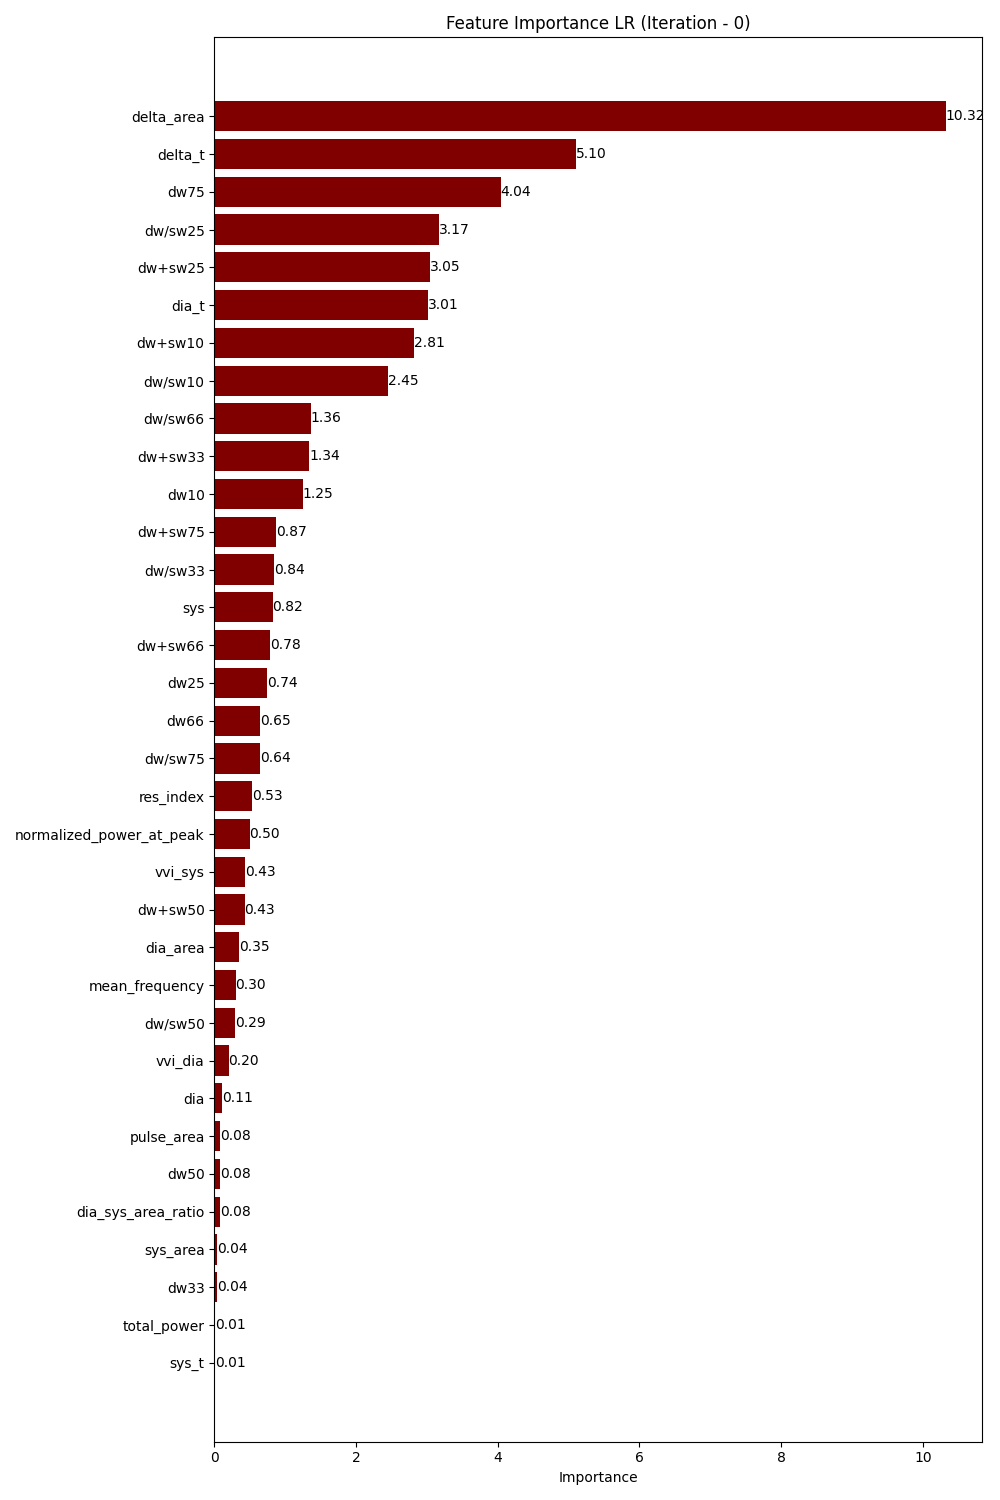
\includegraphics[width=0.82\textwidth]{images/results/feature_importance/feature_importance_plot_LR_0}
    \caption{Feature Importance Chart LR}
    \label{fig:fi_lr}
\end{figure}

\begin{figure}[h]
    \centering
    \vspace{-1cm}
    \hspace{-2cm}
    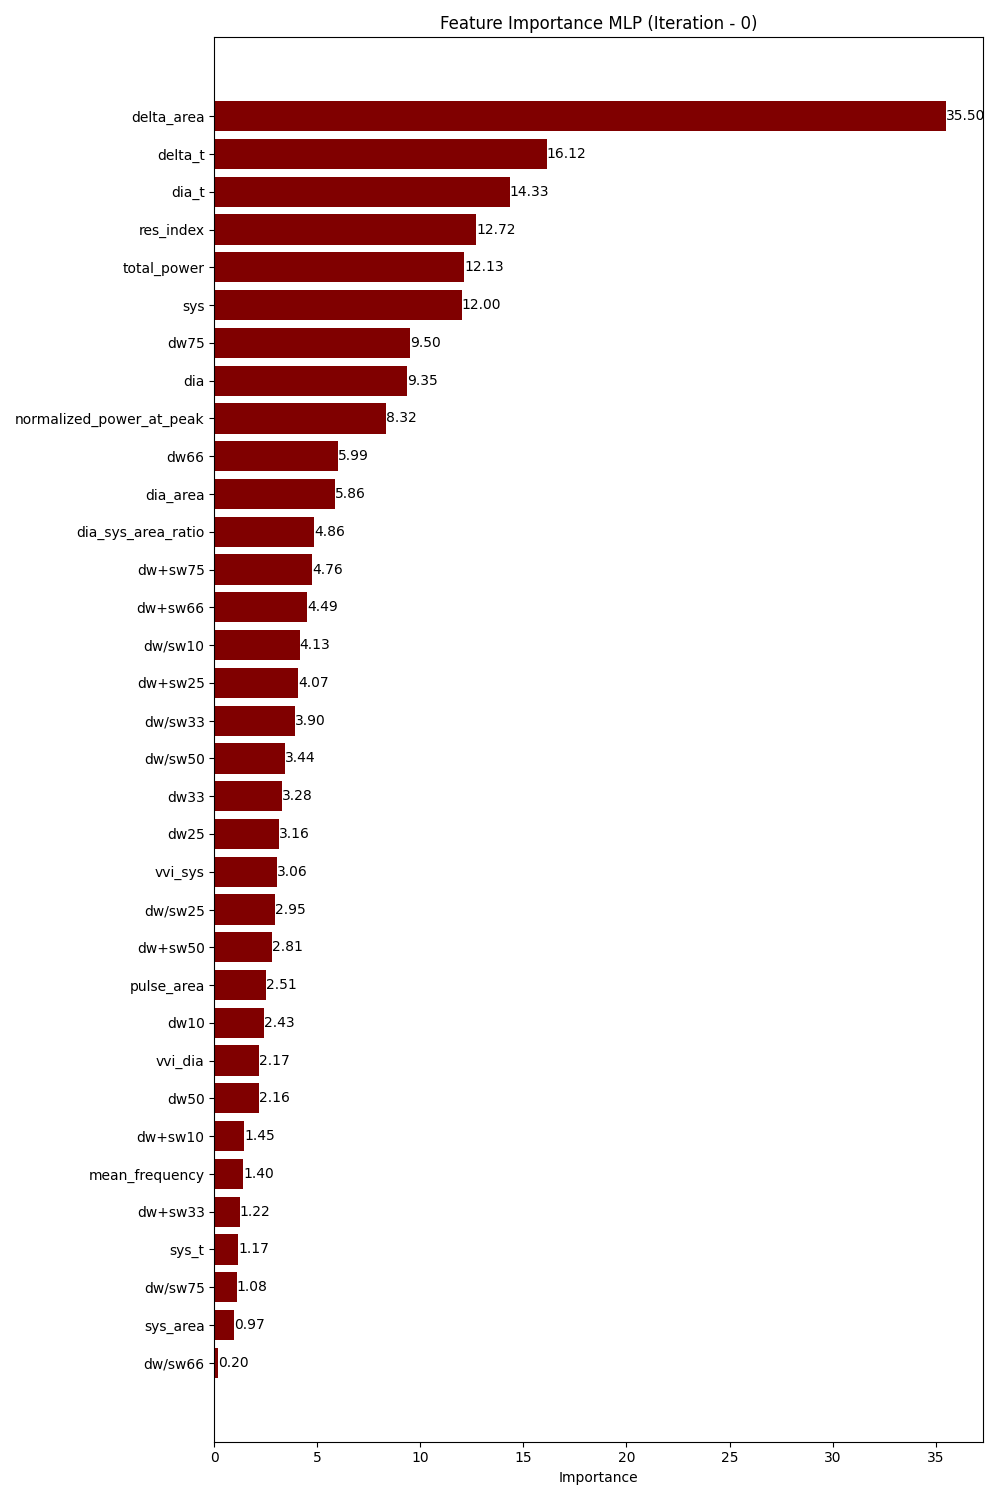
\includegraphics[width=\textwidth]{images/results/feature_importance/feature_importance_plot_MLP_0}
    \caption{Feature Importance Chart MLP}
    \label{fig:fi_mlp}
\end{figure}

\begin{figure}[h]
    \centering
    \vspace{-1cm}
    \hspace{-2cm}
    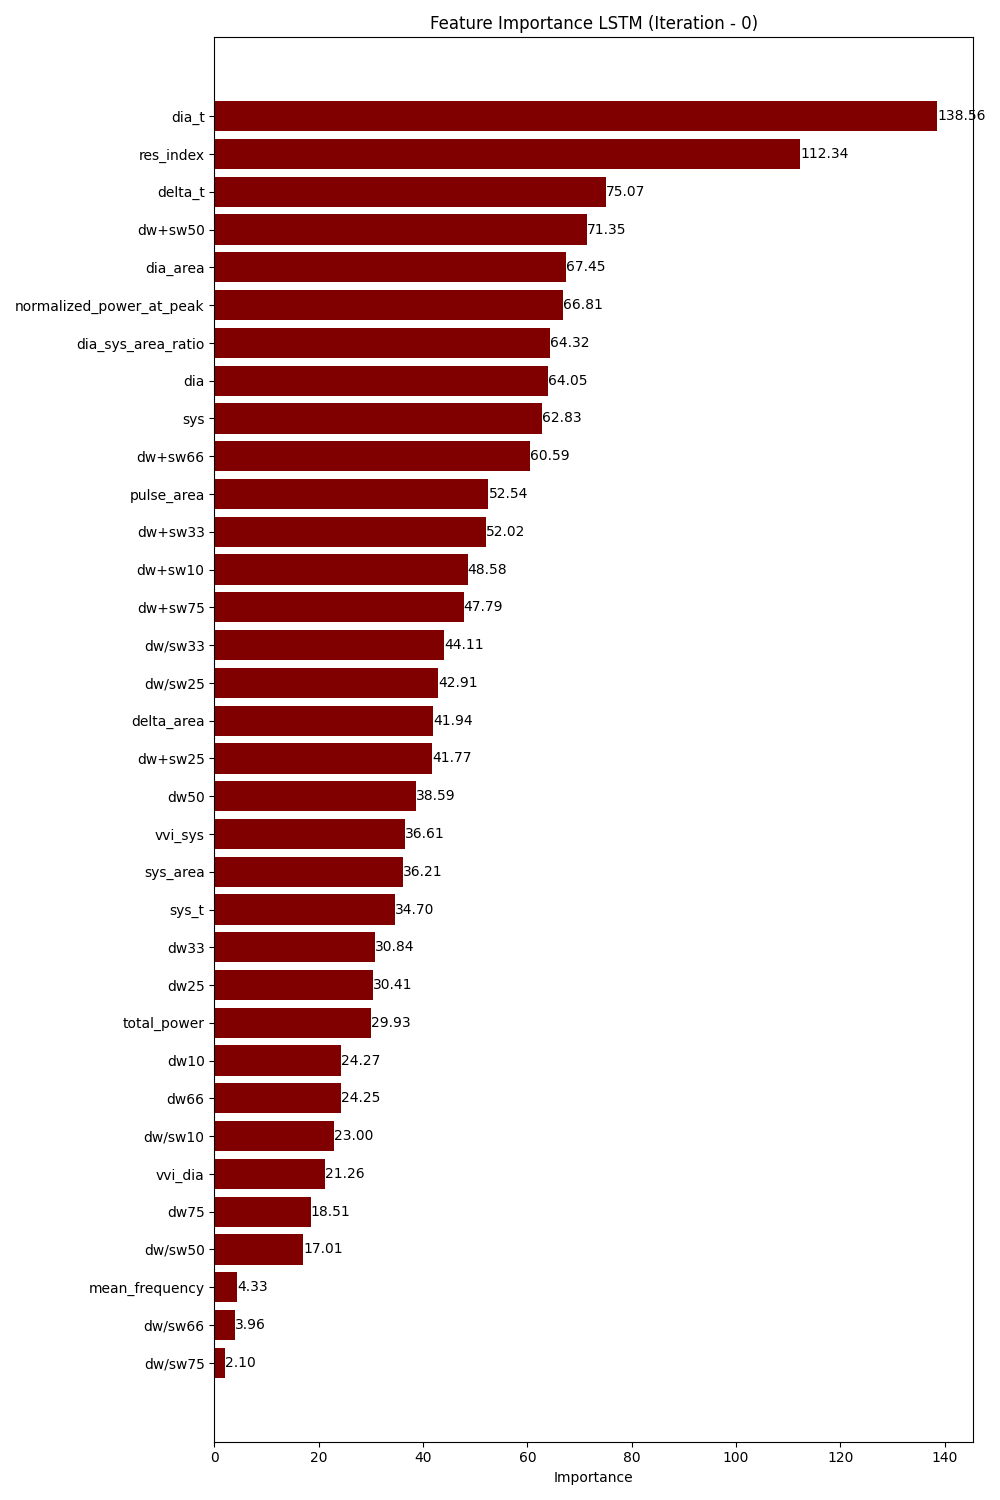
\includegraphics[width=\textwidth]{images/results/feature_importance/feature_importance_plot_LSTM_0}
    \caption{Feature Importance Chart LSTM}
    \label{fig:fi_lstm}
\end{figure}

\begin{figure}[h]
    \centering
    \vspace{-1cm}
    \hspace{-2cm}
    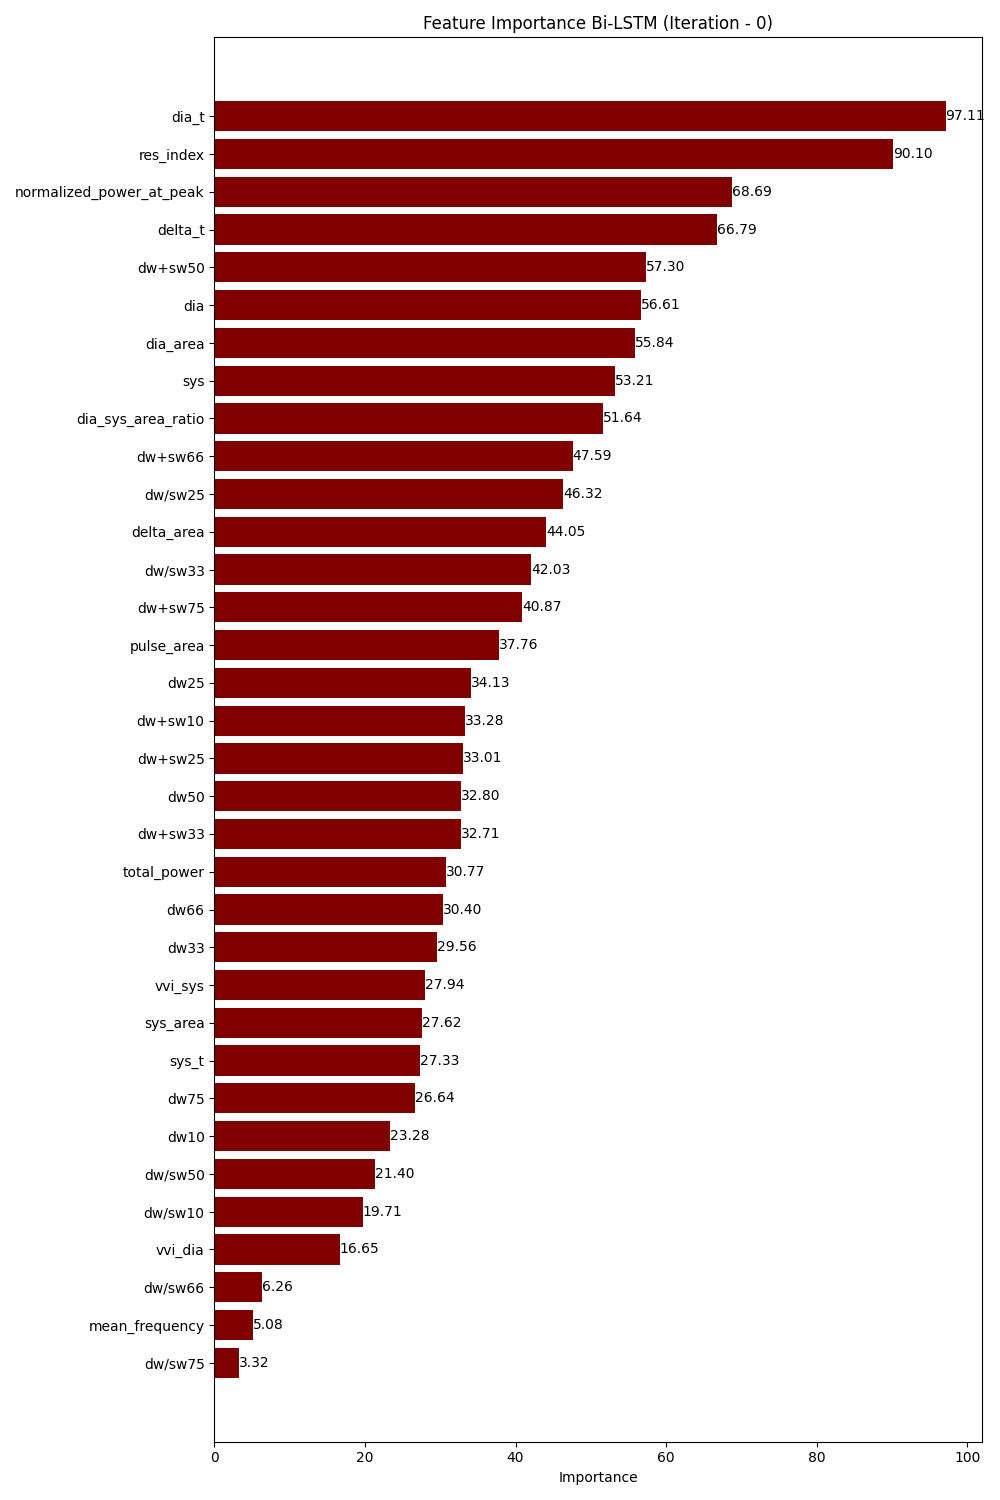
\includegraphics[width=\textwidth]{images/results/feature_importance/feature_importance_plot_Bi-LSTM_0}
    \caption{Feature Importance Chart Bi-LSTM}
    \label{fig:fi_bi_lstm}
\end{figure}

\begin{figure}[h]
    \centering
    \vspace{-1cm}
    \hspace{-2cm}
    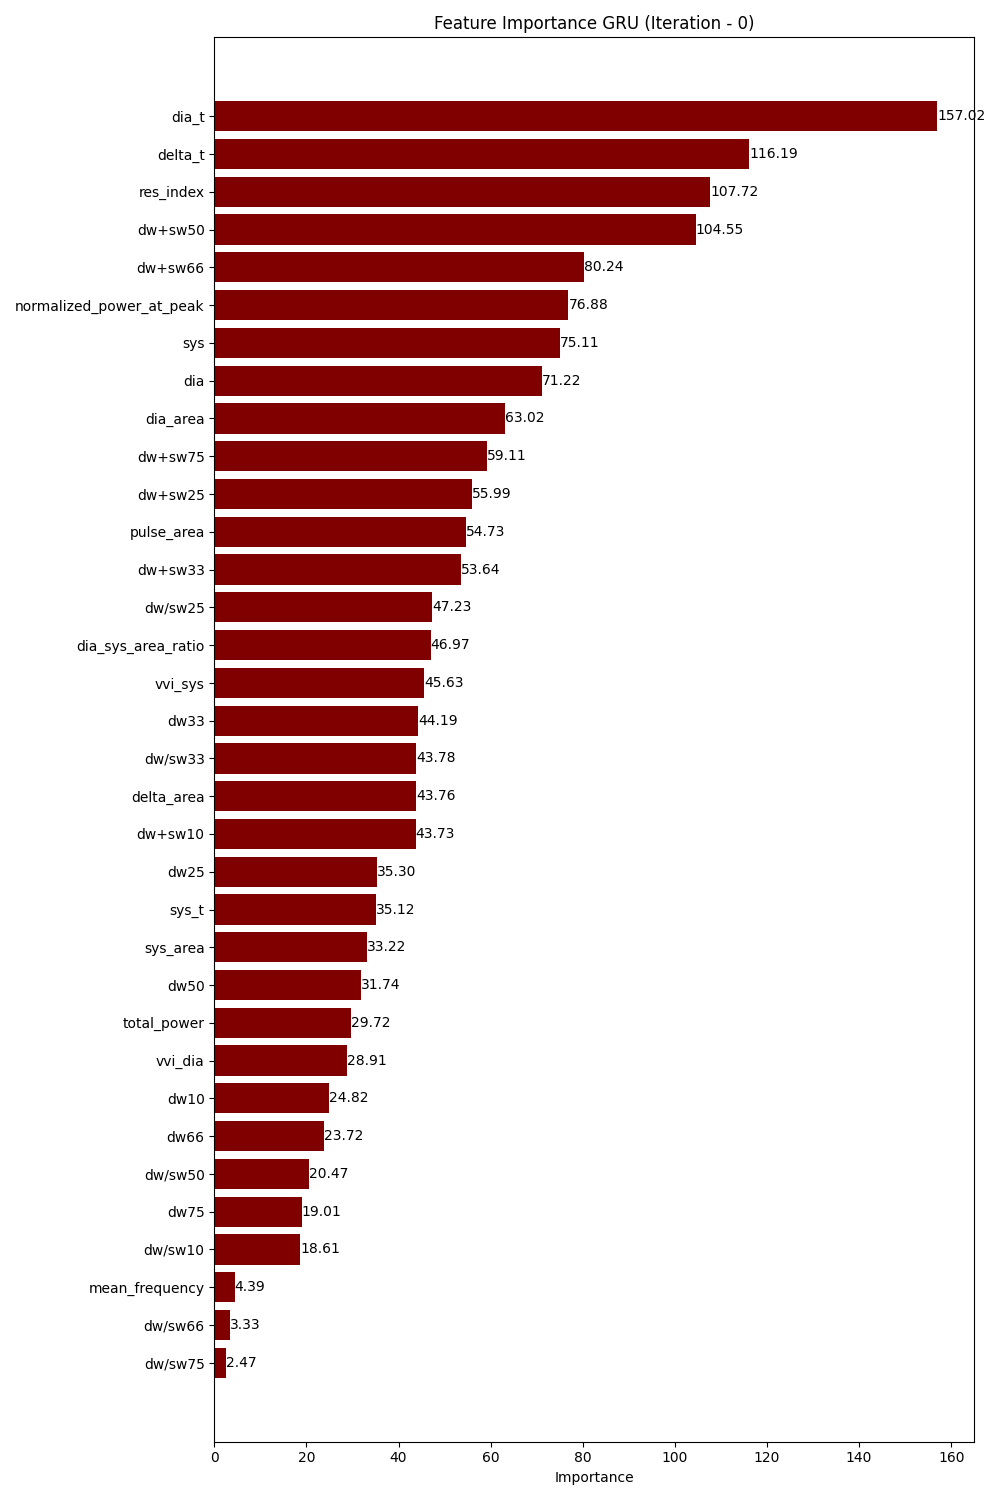
\includegraphics[width=\textwidth]{images/results/feature_importance/feature_importance_plot_GRU_0}
    \caption{Feature Importance Chart GRU}
    \label{fig:fi_gru}
\end{figure}

\begin{figure}[h]
    \centering
    \vspace{-1cm}
    \hspace{-2cm}
    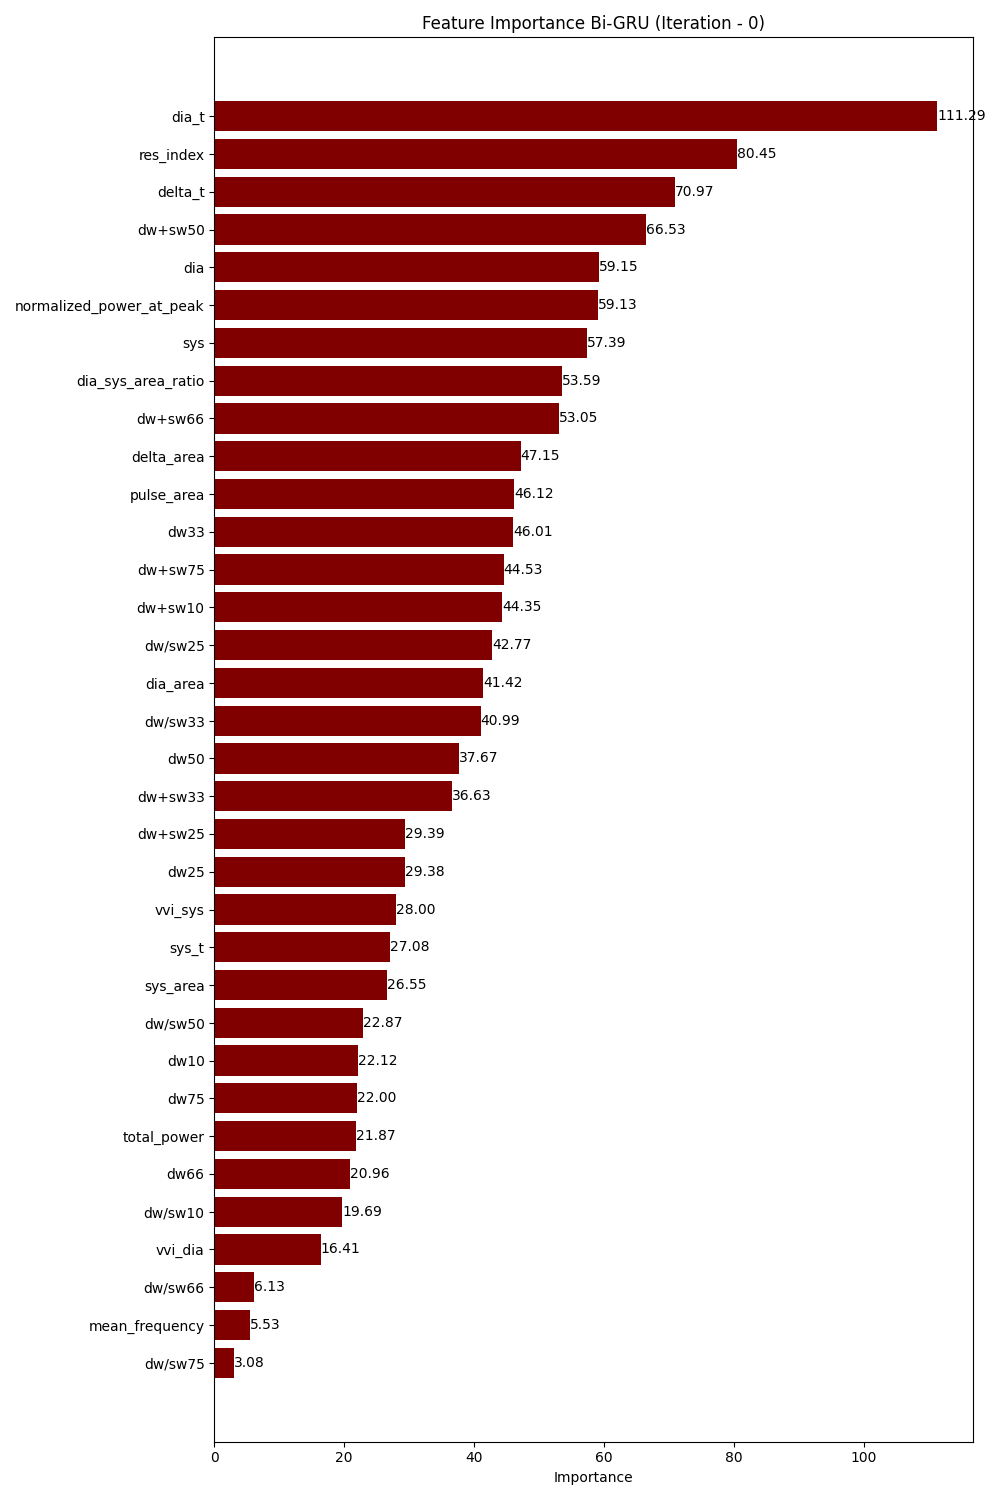
\includegraphics[width=\textwidth]{images/results/feature_importance/feature_importance_plot_Bi-GRU_0}
    \caption{Feature Importance Chart Bi-GRU}
    \label{fig:fi_bi_gru}
\end{figure}

\end{document}